\documentclass [PhD] {uclathes}
%\documentclass [PhD,draft] {uclathes}

\renewcommand{\floatpagefraction}{0.7} 
\renewcommand{\dblfloatpagefraction}{0.7}
%\usepackage[utf8x]{inputenc}

\usepackage{natbib}

\usepackage[
pdfauthor={Mingda Li},
pdftitle={Mingda Li -- PhD Thesis},
pdfsubject={Learning Deep Neuromuscular Control of the Torso for Anthropomimetic Animation},
pdftex, pagebackref, pdfpagelabels, hypertexnames, bookmarks, bookmarksnumbered,
plainpages=false,
naturalnames=false,
pdfpagemode=UseOutlines,
]{hyperref}

\hypersetup{
colorlinks,
citecolor=[rgb]{0.0,0.3,0.0},
filecolor=[rgb]{0.6,0.0,0.0},
linkcolor=[rgb]{0.0,0.0,0.4},
urlcolor=[rgb]{0.0,0.0,0.4}}

\usepackage{setspace} % single-spaces figure cations
\usepackage{multirow}
\usepackage{booktabs} % For formal tables
\usepackage{amsmath, amsthm, bm, amssymb, gensymb}
\usepackage{tikz} \usetikzlibrary{positioning}
\usepackage{graphicx, caption, subcaption}
\usepackage{adjustbox}
\PassOptionsToPackage{draft}{graphicx}
\graphicspath{ {figures-new/}{figures/} }
\usepackage[utf8x]{inputenc} 
\usepackage{romannum}

%%%Negative Sampling
\usepackage{times}
\usepackage{helvet}
\usepackage{courier}
\PassOptionsToPackage{hyphens}{url}
\usepackage{hyperref}
\usepackage{url}
\usepackage{graphicx}
\urlstyle{rm}
\def\UrlFont{\rm}
\frenchspacing
\usepackage{amsthm}


% All commands to check here added by Mingda
\newtheorem{theorem}{Theorem}
\newtheorem{corollary}{Corollary}[theorem]
\newtheorem{lemma}[theorem]{Lemma}
\newtheorem{appendix_theorem}{Theorem}
\usepackage{amsmath,stackengine}
\usepackage{amssymb}
\renewcommand\qedsymbol{$\blacksquare$}
\usepackage{booktabs,subcaption,amsfonts,dcolumn}

\usepackage{latexsym}
\usepackage{balance}
\usepackage{bbm}
\usepackage{url}
\usepackage{mathtools}% Loads amsmath
\usepackage{tablefootnote}

%below library is added by Zijun
\usepackage{breqn} 
%%%Negative Sampling End




\usepackage{color} \definecolor{new-text-color}{rgb}{0,0,255}
\newenvironment{NEW}{\color{new-text-color}}{}


\def\Arrow{\makebox[6.26399pt]{$\blacktriangleright$}~}
\def\Square{\makebox[6.26399pt]{$\blacksquare$}~}
\newcommand{\mat}[1]{\bm{#1}}
\renewcommand{\vec}[1]{\bm{#1}}
\def\diag{\mathop{\mathrm{diag}}}


\usepackage{url}
\usepackage{enumerate}
\usepackage[detect-all]{siunitx}



%%% LLIb

\newcommand{\bldl}{\[\begin{array}{ll}}
% \newcommand{\cldl}{\vspace*{-0.3cm}\[\begin{array}{ll}}
\newcommand{\cldl}{\[\begin{array}{lrcl}}
\newcommand{\eldl}{\end{array}\]}
%\newtheorem{lemma}{Lemma}[section]
\usepackage{mathptmx}
\usepackage{algorithmic, amsmath,graphicx}
\usepackage[ruled,vlined]{algorithm2e}
\usepackage{listings}
\usepackage{subcaption}
\usepackage{booktabs,array}

\newcounter{myrow}
%%% Macros for the guide only %%%
\hyphenation{either}
\providecommand\AMSLaTeX{AMS\,\LaTeX}
\newcommand\eg{\emph{e.g.}\ }
\newcommand{\qr}[1]{\textit{Query #1}}
\newcommand{\ex}[1]{\textit{Example #1}}
\newcommand{\Bi}[1]{\ensuremath{\mathcal{B}_{#1}}\xspace} % the MBS of a partition
\newcommand{\LB}{\ensuremath{\textsf{LB}}\xspace}
\newcommand{\UB}{\ensuremath{\textsf{UB}}\xspace}
\newcommand{\lowb}[1]{\ensuremath{\textsf{LB}_{\mathcal{B}_{#1}}}\xspace}

\newcommand{\return}{\textsf{return}\xspace}
\newcommand{\topk}{top-\ensuremath{k}\xspace}
\newcommand{\simmetrics}{\ensuremath{\sim}\xspace}
\newcommand{\bigo}{\ensuremath{\mathcal{O}}\xspace}

\newcommand\etc{\emph{etc.}}
\newcommand\bcmdtab{\noindent\bgroup\tabcolsep=0pt%
	\begin{tabular}{@{}p{10pc}@{}p{20pc}@{}}}
	\newcommand\ecmdtab{\end{tabular}\egroup}
\newcommand\rch[1]{$\longrightarrow\rlap{$#1$}$\hspace{1em}}
\newcommand\lra{\ensuremath{\quad\longrightarrow\quad}}

%%% LLib ends

\DeclareOldFontCommand{\bf}{\normalfont\bfseries}{\mathbf}

%% dip start

%\usepackage[utf8]{inputenc}
\usepackage{amsmath,stackengine}
\usepackage{color}
\usepackage{colortbl}
%\usepackage{ntheorem}
\usepackage{graphicx}
\usepackage{balance}
\usepackage{tablefootnote}
\usepackage{booktabs,subcaption,amsfonts,dcolumn}
\usepackage{multirow}
\usepackage{indentfirst}
%\theoremseparator{:}
\newtheorem{hyp}{Hypothesis}
%\newcommand{\system}{WASP}
\newcommand{\ie}{{\em i.e.}}

\newcommand{\etal}{{\em et al.}}
\newcommand{\system}{DIP}
\newcommand{\todo} [1]{\textcolor{blue}{{\sf TODO}: #1}}
\newcommand{\sele} [1]{\textcolor{blue}{{\sf CHOOSE}: #1}}
\newcommand{\mingda} [1] {\textcolor{orange}{{\it MingdaCamera}: #1}}
\newcommand{\lume} [1] {\textcolor{blue}{{\it Lume}: #1}}


%%% dip ends


\usepackage{tikz}
\usetikzlibrary{positioning}

\title{Efficient Latent Semantic Extraction from Cross Domain Data with Declarative Language}
%\title{Extracting Latent Semantic Information from Multi-domain Contents by Decalaritive Language and Efficient Algorithm}
% Extracting latent semantic information from abandoned contents/sequences 
% Advanced analytics of abandoned contents/sequences  via declaritive language and efficient algorithm

\author         {Mingda Li}
\department     {Computer Science}
\degreeyear     {2020}

%%%%%%%%%%%%%%%%%%%%%%%%%%%%%%%%%%%%%%%%%%%%%%%%%%%%%%%%%%%%%%%%%%%%%%%%

\chair          {Junghoo Cho}
\chair			{Carlo Zaniolo}
\member         {Yizhou Sun}
\member         {Yingnian Wu}


%%%%%%%%%%%%%%%%%%%%%%%%%%%%%%%%%%%%%%%%%%%%%%%%%%%%%%%%%%%%%%%%%%%%%%%%

\dedication     {\textsl{To my mother, father and girl friend.}}

%%%%%%%%%%%%%%%%%%%%%%%%%%%%%%%%%%%%%%%%%%%%%%%%%%%%%%%%%%%%%%%%%%%%%%%%

\acknowledgments {
	
First and foremost, I would like to thank my  advisors, Professor Junghoo Cho and  Professor Carlo Zaniolo.  Professor Junghoo  has been an exceptional advisor. He is my first mentor in the natural language processing field. Over the years, he gave me extremely visionary advice, generous support and timely feedbacks. His research foresight and ambition greatly motivated me. For each of my projects, he enthusiastically provided insightful suggestions and related articles.   For each of my papers, he patiently point out logic flaws  and unclear descriptions.  I also feel so fortunate to have Professor Carlo as my co-advisor. His professional expertise and brilliant ideas  guided me to resolve many challenging problems. He spent his valuable time teaching me how to come up an idea to satisfy urgent needs in academy, establish a system to implement the idea, and to illustrate findings with concrete examples. 

I would also thank Professor Yizhou Sun and Professor Yingnian Wu  for agreeing to be on my committee and providing their valuable time and  advice  on my research. 

I would thank Tyson Condie for offering me the precious opportunity to join UCLA  CS department as a PhD student and offering funding support to my research. During the early years, he  taught me the way of thinking as a system researcher. He showed me the frontier of distributed system research. He is quite smart and experienced. I could always get innovative thoughts while discussing with Tyson.

It is a great honour to work in ScAi lab. I would thank the whole UCLA ScAi group, especially Matteo Interlandi, Youfu Li, Zijun Xue, Jiaqi Gu, Jin Wang, Muhao Chen, Manoj Reddy, Ling Ding, Xuelu Chen, and Shi Gao who helped me at various times.  

I also want to thank all staff members of UCLA Computer Science Department, especially Joseph Brown, who helped me a lot for various questions I have ever met. 

I have ever done four marvelous internships at Teradata, Nec Laboratories, AWS RedShift and  Alexa AI, where I learned a lot from many remarkable people. I want to  thank my mentors in Nec Laboratories, Cristian Lumezanu and Bo Zong for their guidance on IP embedding project. I want to thank Chengwei Su, Weitong Ruan, Xinyue Liu, Luca Soldaini, Wael Hamza and Fan Yang
for their assistance and  participation in the spoken language understanding project. I also want to thank Yi Xia, Emiran Curtmola, Chainani Naresh, Gaurav Saxena for their generous support. 

Lastly but most importantly, I own my parents and my girlfriend a debt of gratitude.  Without their unconditional love and unbounded support, I cannot remain true to my original aspiration, keep pressing ahead and get through all those hard times. 











}

%%%%%%%%%%%%%%%%%%%%%%%%%%%%%%%%%%%%%%%%%%%%%%%%%%%%%%%%%%%%%%%%%%%%%%%%

\vitaitem   {2011-2015}
{B.S. Computer Science and Technology\\
Harbin Institute of Technology\\
Harbin, China}
\vitaitem  {2015–2016} 
{Research Assistant\\
ScAi Laboratory\\
University of California, Los Angeles\\
Los Angeles, California}
\vitaitem   {2016–2020}
{Teaching Assistant\\
Computer Science Department\\
University of California, Los Angeles\\
Los Angeles, California}
\vitaitem   {2016}
{Research Intern\\
	Teradata\\
	Los Angeles, US}
\vitaitem   {2017}
{Research Intern\\
	NEC Lab\\
	Princeton, US}
\vitaitem   {2018}
{SDE Intern\\
	Amazon AWS Redshift\\
	Palo Alto, US}
\vitaitem   {2019}
{Applied Scientist Intern\\
	Amazon Alexa AI\\
	Boston, US}
\vitaitem   {}
{}
%%%%%%%%%%%%%%%%%%%%%%%%%%%%%%%%%%%%%%%%%%%%%%%%%%%%%%%%%%%%%%%%%%%%%%%%

\publication{Mingda Li, Weitong Ruan, Xinyue Liu, Luca Soldaini, Wael Hamza, Chengwei Su. ``Improving Spoken Language Understanding By Exploiting ASR N-best Hypotheses.'' ArXiv 2020. To be submitted to \emph{SLT 2021}}

\publication{Mingda Li*, Zijun Xue*, Junghoo Cho. ``Amplified Negative Sampling: Sample-Efficient Training for a Large-Class Classifier.'' In review by the \emph{KDD 2020}}

\publication{Jin Wang, Chunbin Lin, Mingda Li, Carlo Zaniolo. ``Boosting Approximate Dictionary-based Entity Extraction with Synonyms.'' Accepted by \emph{Information Sciences Journal 2020}}


\publication{Mingda Li, Weitong Ruan, Xinyue Liu, Luca Soldaini, Wael Hamza, Chengwei Su. ``Multi-task Learning of Spoken Language Understanding by Integrating  N-Best Hypotheses with Hierarchical Attention.'' To be submitted to \emph{COLING 2020}}

\publication{Mingda Li, Jin Wang, Youfu Li, Carlo Zaniolo. ``LLib and LFrame: Logical Libraries and DataFrames for More Expressive Logical Programming.''  To be submitted to \emph{ICLP 2020}}


\publication{Jin Wang, Jiacheng Wu, Mingda Li, Jiaqi Gu, Ariyam Das, Carlo Zaniolo. ``Formal Semantics and High Performance in Declarative Machine Learning using Datalog.'' In review by \textit{VLDB Journal 2020}}

\publication{Mingda Li, Cristian Lumezanu, Bo Zong, Haifeng Chen. ``Learning-based spoofing detection.'' In review by the \emph{EuroS\&P WTMC 2020}}

\publication{Jin Wang, Chunbin Lin, Mingda Li, Carlo Zaniolo. ``An Efficient Sliding Window Approach for Approximate Entity Extraction with Synonyms.'' Accepted by \emph{EDBT 2019 }}

\publication{Carlo Zaniolo, Ariyam Das, Jiaqi Gu, Youfu Li, Mingda li, Jin Wang. ``Monotonic Properties of Completed Aggregates in Recursive Queries.''  \emph{ArXiv 2019}}

%\publication{Cristian Lumezanu, Nipun Arora, Haifeng Chen, Bo Zong, CHO Daeki, Mingda Li. ``Network endpoint spoofing detection and mitigation.'' US Patent App. 16/101,815, 2019.}

\publication{Ariyam Das, Youfu Li, Jin Wang, Mingda Li, Carlo Zaniolo. ``BigData Applications from Graph Analytics to Machine Learning by Aggregates in Recursion.'' Accepted by \emph{ICLP 2019}}

%\publication{Cristian Lumezanu, Nipun Arora, Haifeng Chen, Bo Zong, CHO Daeki, Mingda Li. ``Network endpoint spoofing detection and mitigation.'' US Patent App. 16/101,815, 2019.}


%\publication{Cristian Lumezanu, Nipun Arora, Haifeng Chen, Bo Zong, CHO Daeki, Mingda Li. ``Neural network based spoofing detection.'' US Patent App. 16/101,794, 2019.}

%\publication{Cristian Lumezanu, Nipun Arora, Haifeng Chen, Bo Zong, CHO Daeki, Mingda Li. ``Network gateway spoofing detection and mitigation.''US Patent App. 16/101,834, 2019.}



\publication{Mingda Li, Cristian Lumezanu, Bo Zong, Haifeng Chen. ``Deep Learning IP Network Representations'' \textbf{BEST PAPER AWARD} of  \emph{ACM SIGCOMM Big-DAMA 2018}}

\publication{Mingda Li, Cristian Lumezanu, Bo Zong, Haifeng Chen. ``Learning IP Network Representations.'' Accepted by \emph{ACM SIGCOMM CCR 2018}}

\publication{Zijun Xue, Ruirui Li, Mingda Li. ``Recent Progress in Converesational AI.'' \emph{KDD Conversational AI workshop 2018}}


\publication{Youfu Li, Mingda Li, Ling Ding, Matteo Interlandi . ``RIOS: Runtime Integrated Optimizer for Spark.'' Accepted by \emph{SOCC 2018}}

\publication{Muhammad Ali Gulzar, Matteo Interlandi, Xueyuan Han, Mingda Li, Tyson Condie, Miryung Kim. ``Automated Debugging in Data-Intensive Scalable Computing.'' Accepted by \emph{SOCC 2017}}




%%%%%%%%%%%%%%%%%%%%%%%%%%%%%%%%%%%%%%%%%%%%%%%%%%%%%%%%%%%%%%%%%%%%%%%%

\abstract{
	With large amounts of data continuously generated by intelligence devices,  efficiently analyzing huge data collections to unearth valuable insights has become one of the most elusive challenges for both academia and industry. 
%	both academy and industry are motivated to develop powerful algorithm
	%the big data analytics  to unearth valuable insights from huge data has motivated both academy and industry to develop scalable algorithms  . 	
	The key elements to  establishing a scalable analyzing framework should involve 
    (1) an intuitive interface to describe the desired outcome, 
    (2) a well-crafted model that integrates all available information sources to derive the optimal outcome 
    and (3) an efficient algorithm that performs the data integration and extraction within a reasonable amount of time.
    %a well-proposed algorithm to integrate all available 
	%an optimal training strategy  
	%and a declarative developing interface.
	In this dissertation, 
	we address these challenges by proposing  (\romannum{1})   a cross-language interface for a succinct expression of recursive queries, (\romannum{2}) a domain specific neural network model that can incorporate information of multiple modality, and (\romannum{3}) a sample efficient training method that can be used even for an extremely-large output-class classifiers.
	
	%we focus on the comprehensive enhancement through the scalable analyzing framework by  (\romannum{1})  domain-specific framework designs to enrich the captured information, (\romannum{2})  a sample-efficient training method adaptive to a wide variety of multi-class classifiers with extreme large output-class size, and (\romannum{3}) a cross-language interface for succinct expressions of recursions  in advanced analytics.  
	
	
	
	%A series of challenges are contained in each of the three elements, which we want to address. 
	Our contributions in this thesis are thus threefold: 
	First, for the ubiquitous recursive queries in advanced data analytics, on top of BigDatalog and Apache Spark, we design a succinct and expressive analytics tool encapsulating  the functionality and classical  algorithms of Datalog, a quintessential logic programming language.  We provide the Logical Library (LLib), a Spark MLlib-like high-level API supporting a wide range of recursive algorithms and the Logical DataFrame (LFrame), an extension to Spark DataFrame supporting both relational and logical operations. The LLib and LFrame enable smooth collaborations between logical applications and  other Spark libraries and cross-language  logical programming in Scala, Java, or Python.  
	Second, we utilize  variants of recurrent neural network (RNN)  to incorporate some enlightening sequential information overlooked by the conventional works in two different domains including Spoken Language Understanding (SLU) and Internet Embedding (IE). In SLU, we address the problem caused by solely relying on the first best interpretation (hypothesis) of an audio command through a series of new architectures comprising bidirectional LSTM and pooling layers to  jointly utilize the other hypotheses'  texts or embedding vectors, which are neglected but with valuable  information missed by the first best hypothesis. In IE, we propose the DIP, an extension of RNN, to build up the internet coordinate system with the  IP address sequences, which
	are also unnoticed in conventional distance-based internet embedding algorithms but encode structural information of the network.  Both DIP and the integration of all hypotheses bring significant performance improvements for the corresponding downstream tasks.
	Finally, we investigate the training algorithm for multi-class classifiers with a large output-class size, which is common in deep neural networks and typically implemented as a softmax final layer with one output neuron per each class. To avoid expensive computing the intractable normalizing constant of softmax for each training data point, we  analyze the well-known negative sampling and improve it to the amplified negative sampling algorithm, which gains much higher performance with lower training cost.
	
	
	
	
	
	
%    In the first part, we aim to utilize the variants of recurrent neural network (RNN)  to incorporate some enlightening sequential information overlooked by the previous works in different domains and tasks. 
%    We find, 
%%	However, in reality, we may find the provided algorithm could overlook  or  hardly integrate some enlightening information within its framework. For e.g., 
%	in Spoken Language Understanding, only the best of automatic speech recognition (ASR)  interpretations (hypotheses) for  an input audio signal is utilized to understand the intent, while the rest hypotheses containing fragmented important messages are ignored. We investigate a series of  methods to jointly utilize top $n$ interpretations by integrating the hypothesized text or hypothesis embedding vectors with BiLSTM and achieve significant accuracy improvements for intent or domain classification.   
%	 Similarly, while embedding  the Internet structure,  only the distances among IP address are utilized to build up the network coordinate system  but the information contained by the  IP address  is unnoticed. 
%	% Since the RNN and its variants have been proven to be effective to capture causal and/or contextural information from sequantial data, we extend them to incorporate the information from sequences of spoken words or IP bits. 
%	We propose the DIP, a deep learning based framework for IP network representations, which normalizes each IP address to seperate sequences by the volume of contained routable information within IP bits and exploits a variant of RNN for a low-dimensional representation.  
%	
%	In the second part, we investigate the training algorithm for multi-class classifiers with a large output-class size, which is common in deep neural networks and typicaly implemented as a softmax layer in the final layer 
%	 %like natural language generation with  a softmax layer as final layer 
%	 containing one output neuron per each word. 
%%	The multi-class classifier  is very common in deep neural networks. For example, in the natural language generation or graph embedding models, the final layers are  always implemented  as a softmax layer  with one output neuron per each word or node, which can be as large as the size of the whole dictionary or graph.  
%	It is prohibitively to calculate the intractable normalizing constant of softmax for each training data point. We analyze the well-known negative sampling and propose the amplified negative sampling algorithm, which gains higher performance with lower training cost. 
%	
	% explore the DNN frameworks to for internet embedding and  
	
	% However, in reality, we may find: the provided algorithm could overlook  or can hardly integrate some enlightening information within its framework; the training process can  be computationally intensive; and the expressing of complex logic computations could be complicated. 
%	In this thesis, we tackle those problems separately by novel information integration architectures, a sample-efficient training algorithm and a decalrative logical programming interface expressing complex logic.
	
	 
	% improve each component by demonstrating novel algorithms or expressive languages. 
	
	%Some of the bottlenecks for scalable analyzing involve the deficiency of proposed algorithm to integrate all the available data, the computationally intensive learning process of the algorithm, alyzed the complicated development for   complex logic computations. In this thesis, we 
	
	%a well-designed architecture to integrate all the available features, an inexpensive  
}

%%%%%%%%%%%%%%%%%%%%%%%%%%%%%%%%%%%%%%%%%%%%%%%%%%%%%%%%%%%%%%%%%%%%%%%%

\begin{document}
\makeintropages

%%%%%%%%%%%%%%%%%%%%%%%%%%%%%%%%%%%%%%%%%%%%%%%%%%%%%%%%%%%%%%%%%%%%%%%%


%In the first part, we aim to utilize the variants of recurrent neural network (RNN)  to incorporate some enlightening sequential information overlooked by the previous works in different domains and tasks. 
%We find, 
%	However, in reality, we may find the provided algorithm could overlook  or  hardly integrate some enlightening information within its framework. For e.g., 
%in Spoken Language Understanding, only the best of automatic speech recognition (ASR)  interpretations (hypotheses) for  an input audio signal is utilized to understand the intent, while the rest hypotheses containing fragmented important messages are ignored. We investigate a series of  methods to jointly utilize top $n$ interpretations by integrating the hypothesized text or hypothesis embedding vectors with BiLSTM and achieve significant accuracy improvements for intent or domain classification.   
%Similarly, while embedding  the Internet structure,  only the distances among IP address are utilized to build up the network coordinate system  but the information contained by the  IP address  is unnoticed. 
% Since the RNN and its variants have been proven to be effective to capture causal and/or contextural information from sequantial data, we extend them to incorporate the information from sequences of spoken words or IP bits. 
%We propose the DIP, a deep learning based framework for IP network representations, which normalizes each IP address to separate sequences by the volume of contained routable information within IP bits and exploits a variant of RNN for a low-dimensional representation.  

%In the second part, we investigate the training algorithm for multi-class classifiers with a large output-class size, which is common in deep neural networks and typicaly implemented as a softmax layer in the final layer 
%like natural language generation with  a softmax layer as final layer 
%containing one output neuron per each word. 
%	The multi-class classifier  is very common in deep neural networks. For example, in the natural language generation or graph embedding models, the final layers are  always implemented  as a softmax layer  with one output neuron per each word or node, which can be as large as the size of the whole dictionary or graph.  
%It is prohibitively to calculate the intractable normalizing constant of softmax for each training data point. We analyze the well-known negative sampling and propose the amplified negative sampling algorithm, which gains higher performance with lower training cost. 

% explore the DNN frameworks to for internet embedding and  

% However, in reality, we may find: the provided algorithm could overlook  or can hardly integrate some enlightening information within its framework; the training process can  be computationally intensive; and the expressing of complex logic computations could be complicated. 
%	In this thesis, we tackle those problems separately by novel information integration architectures, a sample-efficient training algorithm and a decalrative logical programming interface expressing complex logic.


% improve each component by demonstrating novel algorithms or expressive languages. 

%Some of the bottlenecks for scalable analyzing involve the deficiency of proposed algorithm to integrate all the available data, the computationally intensive learning process of the algorithm, and the complicated development for   complex logic computations. In this thesis, we 

%a well-designed architecture to integrate all the available features, an inexpensive  

\chapter{Introduction}


\section{Motivations}
In the big data era, we have witnessed the rising demand of efficiently and conveniently extracting insights  from large-scale data sets for decision making in different domains. The demand has driven researchers to propose various  neural network-based algorithms revolutionizing many fields, ranging from image processing \citep{he2016deep}, natural language processing \citep{devlin2018bert} to speech recognition \citep{amodei2016deep}, etc. In addition, the big data anlytics and machine learning platforms like PyTorch \citep{paszke2019pytorch}, Tensorflow~\citep{abadi2016tensorflow} and Apache Spark~\citep{zaharia2010spark} are continuously built up in open source and commercial markets, to provide maximal flexibility and speed while implementing the analyzing pipeline with existing or user-defined algorithms. 
%For large data processing, some steps may 

Although the huge success has been achieved, for the advanced analytics on scalable data sets, there are still some challenges and ongoing efforts to tackle them, including:
\begin{itemize}
	
	\item \textbf{Integrating more information.} While great efforts have been dedicated to assimilate massive amounts of data for analysing algorithms, only a tip of the big data iceberg has been utilized during analysing. 
	To make full use of the assimilated data, researchers design novel architectures of algorithms like the bi-directional RNN \citep{graves2013speech} to exploit the backward information, and involve more tasks for training like the masked language model and next sentence prediction mentioned in Bert \citep{devlin2018bert}.
	
	In two of the fastest growing areas in  computer science, the internet embedding and spoken language understanding, we find some enlightening information not considered in the existing analyzing pipeline, which makes  the performance of corresponding downstream tasks non-optimal. Currently, while embedding the internet structure,  only a single source of structural data among IP addresses like hop counts ~\citep{barford-sigcomm,barford-infocom} is utilized to build up the network coordinate system. We realize the IP address of the host in internet, a sequence of bits, could provide a coarse indication of the location of the host, but is overlooked by current internet embedding techniques. As for understanding the speech, only the recognition result (hypothesis) of an input speech with highest ASR confidence score \citep{tur2011spoken} or reranking score \citep{peng2013search, morbini2012reranking} is relied and transferred to the natural language understanding (NLU) module for domain or intent classification.  We find the first best hypothesis can be noisy, while the other hypotheses can be more similar to the  ground-truth transcription of the speech. Driven by the above findings, we would like to propose novel frameworks involving the unnoticed information for a better performance in downstream tasks. 
	 % but the information contained by the  IP address sequences  is unnoticed. 
	
	\item \textbf{High training cost for large-class classification.} Among all the analysing algorithms, the neural networks with numerous layers and parameters are recently widely utilized  in different domains due to their strength at learning features at different levels of data abstraction for a better decision making. However, the training could be quite computationally expensive especially when the final layer is a softmax layer for large-class classification (e.g. word embedding, graph embedding), since the cost of standard training algorithm  is proportional to the output class size (e.g. size of words in a dictionary, nodes in a graph).  To tackle the issue, a number of techniques like, negative sampling \citep{mikolov2013efficient}, hierarchical  softmax \citep{morin2005hierarchical}, adaptive softmax \citep{bengio2008adaptive,rawat2019sampled} , are developed.
	
	Negative sampling is one of the most popular techniques utilized in practice due to its simplicity and efficiency. Experimental observations show that a larger negative sample size can achieve a better downstream task performance. However, the training cost is more expensive for a larger sample size. Could we get the best of the two worlds? This dream motivates us to analyze the technique and further amplify the negative sampling to get a higher performance with unchanged or even smaller sample size. 
	
	%We careful analyze the technique, and find the implication of negative sampling. Based on 
	

	
	\item \textbf{Complicated expression of recursion.} Recursions are ubiquitous in advanced data analytics, such as graph analytics,  
	data mining algorithms. An efficient development of a complicated recursive algorithm on the well-known data analytics platforms like Apache Spark requires deep understanding of the algorithm and platform's libraries. To simplify the development,  a renaissance of interest has been brought to Datalog, a declarative logic programming language, for its succinct expression of recursions. Numerous of Datalog systems including DeALS \citep{yang2015parallel}, BigDatalog \citep{shkapsky2016big}, RaSQL \citep{gu2019rasql} are built up but there is still space for improvement on usability and interoperability.
	%the rule-based logical programming is considered. 
	%A series of declarative programming languages like 
	
	Most of the conventional Datalog systems adopt the Datalog syntax, which requires a deep understanding of logical programming. Recently, this is realized by RaSQL, which proposes a simple extension of  SQL syntax to improve the usability.  However, for a wider audience from data science community, should it be better to  provide a  data scientists' familiar cross-language API encapsulating a wide range of Datalog algorithms like Spark MLlib? For a flexible developing, is it possible to support the logical operations within a DataFrame-like  data structure? These two questions stimulate us for a better Datalog-based data analytics tool design.

\end{itemize}

\section{Contributions}
All the contributions of this thesis center around  the aforementioned motivations and are summarized as follows:
\begin{itemize}
	\item We realize and experimentally show  the structural information contained in IP addresses for internet embedding and propose a deep learning based framework, DIP, to utilize the information. To the best of our knowledge, DIP is the first framework to predict distance (or hop count) to arbitrary IPs (even unknown hosts i.e., not contained in training data) based only on the value of their IP address and routable prefix without any other domain knowledge.
	\item We further explore the impact of deep learning in the network  security area by using network embeddings to learn IP maps for spoofing detection. We  combine the DIP with the hop count filtering, a well-known map-based spoofing detection mechanism, which maps each IP to a hop count value for one target IP address and is restricted to the detection on specific targets. The new framework can help any Internet server detect packets spoofed with any IP address without any additional measurements to that IP.
	\item We pioneer the spoken language understanding research on jointly utilizing all hypotheses from ASR module. We investigate the exact matching between hypotheses and the ground-truth transcription of the input speech, which reveals the value contained in the 2$^{nd}-n^{th}$ best hypotheses. To involve more than one hypothesis during NLU, we introduce a series of simple yet efficient models and significantly improve the SLU system robustness to the noises from  ASR module. 
	\item We take the effort to efficiently train the high computational cost large-class classifiers. We propose a new sample-efficient training algorithm, amplified negative sampling (ANS). We theoretically and experimentally demonstrate  that the ANS leads to the higher-accuracy model of a larger sample size without paying its high computational cost.
	\item Finally, we design a cross-language (Python, Scala, or Java) Datalog programming interface with two important components, LLib and LFrame. LLib is a high-level logical library, providing the encapsulation of a wide range of Datalog algorihtms.  LFrame is an extension to DataFrame with the functionality of basic logical operations like  definitions of recursive rules. With running examples, we show the simplified development of recursive applications   and flexible collaborations between LLib or LFrame and exisiting Spark libraries.
\end{itemize}



\section{Thesis Outline}

In this dissertation, we mainly address  three of the most important elements of the efficient scalable data analyzing. We firstly explore how to make full use of all information while extracting semantics and insights for decision making. More specifically, in  Chapter \ref{ch:dip}: (a) We propose the DIP, a variant of RNN, for establishing the network coordinate system via embedding the IP address sequence. Compared to the coordinate system built on single source of structural data like latency or hop count, we demonstrate the superiority of DIP for unknown IPs; (b) We show the spoofing detection, one of a wide range of problems the DIP framework can be applicable to, and the benefits from DIP to   significantly reduce cost of achieving complete IP maps. In Chapter \ref{ch:nbest}, we explore the value of unused ASR interpretations and numerous ways to integrate them in the  spoken language understanding system.   

Secondly, we explore how a 
  large-class classifier can be  efficiently trained through a sample-efficient training algorithm in Chapter \ref{ch:nec}. In the chapter, the intuition, theoretical and experimental analysis of the  developed algorithm, amplified negative sampling, are  discussed.  Then, we explore how to design a succinct interface for advanced data analytics with superiority on recursion expressions in Chapter \ref{ch:lib}. We develop a high-level Datalog library, LLib,  for simplified end-to-end recursive application development with existing Datalog algorithms and a data structure, LFrame, for flexibly defining  the logic of a new recursive application. We finally conclude the dissertation and discuss avenues for future work in Chapter \ref{ch:con}.
  
  

%The remainder of the dissertation is organized as follows. In Chapter \ref{ch:dip}, 



\chapter{Extracing Latent  Information from IP Network}
\label{ch:dip}

%We propose to use deep learning on neural networks to learn structural properties of the Internet, such as node clustering or distance between nodes. 
In this chapter, we firstly present \system{}, a deep learning based framework to learn structural properties of the Internet, such as node clustering or distance between nodes, from the IP addresses. 
%
Existing embedding-based approaches use linear algorithms on a single source of data, such as latency or hop count information, to approximate the position of a node in the Internet.
%
In contrast, \system{} computes low-dimensional representations of nodes that preserve structural properties and non-linear relationships across multiple, heterogeneous sources of structural information, such as IP, routing, and distance information.
%
%In particular, given training data including IP address values, routing information, and hop count data, \system{} is optimized to compute low-dimensional vector representations for hosts so that both local (\eg{}, clusters of hosts) and remote (\eg{}, distances to other hosts) structural properties are well preserved.
%
Using a large real-world data set, we show that \system{} learns representations that preserve the real-world clustering of the associated nodes and predicts distance between them more than 30\% better than a mean-based approach. 
%
Furthermore, \system{} accurately imputes hop count distance to  unknown hosts (\ie{}, not used in training) given only their IP addresses and routable prefixes.
%We introduce \system{}, a neural network that computes a low-dimensional vector representation for any host in the Internet that preserves both local (\eg{}, clusters of hosts) and remote (\eg{}, distances to other hosts) structural properties. We train \system{} using . Using a large real-world data set we show that \system{} representations preserve the real-world clustering of the associated hosts and predict distance between hosts50\% better than a mean-based approach. Furthermore, we are able to compute distance to new hosts (\ie{}, not using in training) given only their IP address and only with a small loss in accuracy.
Our framework is extensible to new data sources and applicable to a wide range of problems in network monitoring and security.


Then, we consider an important topic, spoofing defense,  based on the full knowledge of the internet structural properties.  Map-based IP spoofing defenses associate source IPs to immutable structural properties of the Internet, such as paths, hop counts, or neighbors to a target, and filter out packets whose header information does not match the maps. Although accurate, existing methods lack sufficient coverage. Network maps on AS border routers do not detect spoofed packets that traverse unprotected networks. Host maps at the edge protect only against spoofed packets with source IPs known by the host. 
%
We propose to learn IP maps by constructing a structural model (or embedding) of the Internet from a limited number of measurements.  
%
We study the feasibility of learned IP maps by combining hop count filtering, a known map-based spoofing defense mechanism that maps IPs to hop counts to a target, and DIP, a deep learning based learning algorithm that computes vector representations of IPs that preserve hop count distance between them. 
%
Using a large data set of hop counts between Internet hosts, we show that learned maps can detect packets spoofed with almost {\em any} IP address and traversing {\em any} path using an embedding generated from only a few thousand IP addresses and hop counts between them.
%
In addition, our embeddings are general: an Internet model trained for a set of hosts can be used by any other host to generate new IP maps with little loss in accuracy. 

\section{Deep Learning IP Network Representations}
\subsection{Introduction}
\label{dip:intro}

The ability to map, analyze, and understand the structure of the Internet helps network management and operations by revealing opportunities for improvement or potential design flaws. For example, accurately predicting the closest server is critical in peer selection and load balancing~\citep{silkroad}. Knowing how remote IPs are clustered can help diagnose anomalous events such as spoofing attacks~\citep{hc-filter}. A holistic view of the network and its structure is essential towards achieving the  vision of self-driving networks~\citep{self-driving}. 

%The structure of a network consists of several properties such as clustering, distance, or connectivity. 
Most previous attempts to uncover the Internet structure relying on active probing from multiple vantage points using tools such as {\em traceroute} and {\em ping}~\citep{packetlab,rocketfuel}. Such techniques provide fine-grained introspection (\ie{}, can measure specific properties in specific parts of the network, such as the latency of a path) but pose a significant cost in terms of network overhead. 
%

In contrast, embedding-based approaches use fewer, strategic measurements~\citep{vivaldi,barford-sigcomm} or passive observations on network traffic~\citep{barford-imc} to learn vector representations for the network end-hosts in a low-dimensional space. The representations approximate the positions of hosts in the Internet and are used to recover structural network properties, such as distance between nodes or clustering of nodes.
%
However, the complexity of the Internet and the sparse input data make it difficult to compute accurate representations. Oftentimes, embedding approaches rely on additional data sources, which cannot be easily used in the embedding process, to refine and tune the final embeddings. For example, several embedding methods build representations based on distance-based metrics, such as latency or hop count, and then refine (or even replace) the final representations using additional probes or static information such as AS membership or routing information~\citep{vivaldi,barford-infocom}.


The emergence of deep learning as a powerful tool to extract hidden features in data calls for revisiting the problem of learning network representations through embedding. In particular, deep learning techniques provide two key benefits. First, they allow multiple heterogeneous sources of information as input, thereby identifying more accurately the relationships between multiple sources of data that jointly contribute to a specific structural property~\citep{karpathy2015deep,wang2018learning,mikolov2013exploiting}. Second, deep neuron networks are extensible and can easily incorporate additional sources of information by attaching more neurons, network layers, or network branches~\citep{wang2018learning}. One can start with a model trained on the original components and re-train it using only the newly added parts or data sources~\citep{erhan2010does}. This makes it easier for network operators to deploy, apply, or update neural network based models.


We propose \system{}, a deep learning based framework to learn the structure of the Internet. 
\system{} is a ten-layer neural network\footnote{To avoid confusion and unless explicitly stated otherwise, we use {\em network} or {\em Internet} to refer to the physical IP network and {\em neural network} to refer to the neural network we design to learn the structural properties of the physical network} that computes a low-dimensional vector representation for any node\footnote{We use {\em node} or {\em (end-)host} to denote any computer connected to the Internet and assigned an IP address.} in the Internet {\em given only its IP address and routable prefix}. \system{} preserves both local and global structure: clustered  nodes have similar representations and the distance between two representations approximates the hop count between the associated nodes.

We train our neural network using three heterogeneous data sets: hop count distances between Internet nodes, the 32 bits IP address and inter-domain routable prefix information for each node. 
%
A key insight to train \system{} is to {\em first compute representations based on the IP and routing information}, thereby recovering structural information hidden in the IP values, and refine them using a distance-based optimization.
%
As the size of the routable prefix varies by IP, we first normalize the IP and prefix data by representing an IPv4 address on 64, rather than, 32 bits. To capture structural information encoded in the IP address value, we feed the eight bytes of the normalized IP sequentially at each of the first eight layers of the neural network. We then use the last two layers to get the hop count matrix and optimize the embedding distance prediction. With a trained \system{}, we can estimate distance between {\em any} two Internet hosts as long as we have their IPs, even if they are not part of the training data. 

Results on large real-world data sets of hop counts between thousands of IP addresses and 95 geographically distributed servers show that we can predict hop count distance between known hosts (\ie{}, whose IP address were used in the training) with an absolute error of around 2 hops and over 30\% better than a mean-based method. We infer the distance between unknown IPs (\ie{}, not appearing in training data) with a small loss in accuracy compared to known IPs. In addition, the representations learned by \system{} preserve the real-world clustering of the associated hosts. The accuracy of our model increases when we increase the training data set.





%Deep learning provides both a general and an extensible framework to recover and analyze network structure from IP information and sparse distance data. \system can be easily extended to incorporate other sources of structural information, such as AS membership or latency measurements between hosts. We believe 

While our results are preliminary, they offer us a glimpse of the power of deep learning in recovering structural properties of the Internet from sparse data. \system{} is the first framework that can estimate accurately the distance to any Internet host given only its IP address and routable prefix without any distance data.
%To the best of our knowledge, this is the first attempt to learn Internet structural properties from IP address values. While our results are preliminary, they suggest the power of deep learning in identifying hidden features encoded in the value of an IP address



\subsection{Background and Related Work}
\label{dip:background}

\textbf{What is structure?} Many properties can make up the structure of the Internet: connectivity between IPs, routers, or networks; distance-based metrics such as hop count or latency; similarity-based metrics such as the set of one's neighbors in the connectivity graph; path-based properties such as the sequence of routers on a path. Here, we focus on two specific properties that define both the local and the global structure of a network: clustering of end-hosts and hop count based distance between end-hosts. %In Section, we discuss how to extend our approach to other properties.

\textbf{Network coordinate systems} learn vector representations for participating nodes such that the position of the node in the embedding approximates its position in the Internet. Most coordinate systems build embeddings using a single source of structural data: latency measurements among nodes or to predetermined landmark servers~\citep{vivaldi, gnp, pic,pyxida,zhao2011efficient} or hop count information from passive traffic observations~\citep{barford-sigcomm,barford-infocom}. 
%
Latency and hop count data is often sparse and cannot always be accurately embedded in metric spaces. To overcome these issues, several approaches use out-of-band information, such as location~\citep{vivaldi} or routing~\citep{barford-infocom} data, or perform active measurements~\citep{barford-sigcomm} to impute the missing data and detect clusters or distances.
%Because of the sparsity and structulatencies or hop counts cannot be accurately embedded in a metric space, some coordinate systems use location information to tune the embedding~\citep{vivaldi}. In contrast, we propose to train an embedding model using multiple diverse sources of data, including routing and distance information.
%
%Eriksson \etal{} use hop count information from passive traffic observations to build an embedding of the Internet~\citep{barford-infocom}. The hop count represents the number of routers on a path. Similarly to embedding-based approaches, hop count information alone is not sufficient to accurately embed all hosts. The authors resort to active probes~\citep{barford-sigcomm} or AS information~\citep{barford-infocom} to fill in missing hop count data and detect node clusters or distances. 
Unlike them, we propose to train our embedding jointly using distances, routing information and host IP values, thereby learning hidden structural features encoded in a node's IPv4 address. With a trained model, we are able to embed and find the hop count to any IP, without the participation of its host.% \mingda{and able to embed any IP address in IPv4}.

\begin{figure*}[t]
	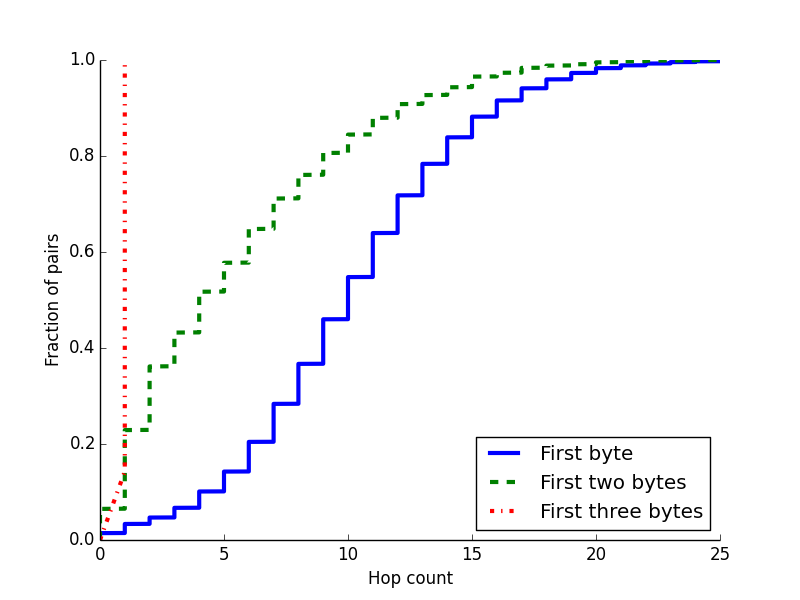
\includegraphics[width=.45\linewidth]{Graph/dip/hopcountbybyte.png}
	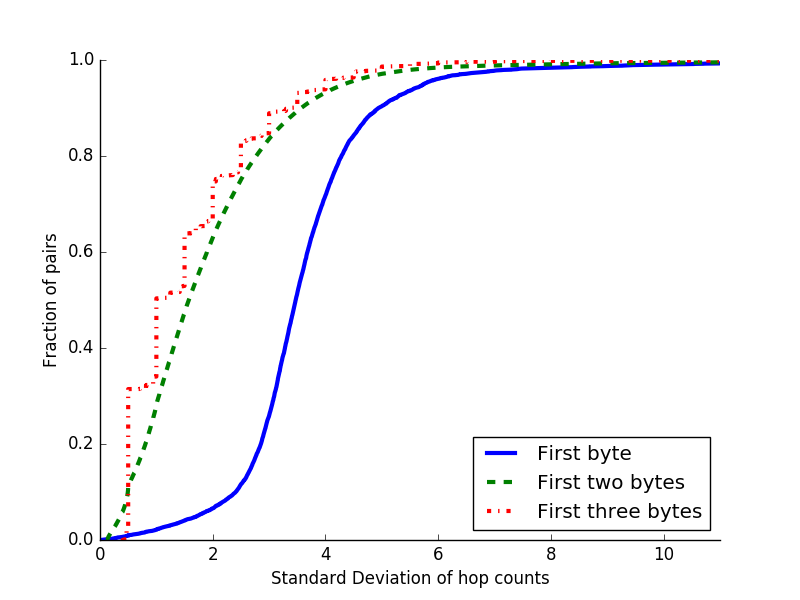
\includegraphics[width=.45\linewidth]{Graph/dip/hopcountSDbyprefix.png}
	\caption{Cumulative distribution of (left) hop counts between pairs of host-server IPs that share the first, first two, or first three bytes, and (right) standard deviation of hop count distribution among groups of IPs sharing the first, first two, or first three bytes. The more similar two IPs are, the closer they are and the more similar their distances to the same third IP are.}
	\label{fig:difference}
\end{figure*}


\textbf{Deep neural networks} consist of multiple layers of interconnected neurons~\citep{lecun2015deep}. A neuron aggregates multiple input values using local weights and biases, applies an activation function, and produces one or more numerical values as output. 
%
Given a training task, one can define an objective function to evaluate the output of the entire neural network, \eg{}, prediction error. 
%
Using gradient-based back-propagation algorithms to optimize the objective function~\citep{kingma2014adam}, neural networks automatically tune the weights and biases of each neuron to achieve a better performance.

%output by passingis a function that takes learning} generally refers to the modeling and training methods for a category of machine learning models called deep neural networks~\citep{lecun2015deep}. Informally, a deep neural network consists of multiple layers of interconnected neurons. Each neuron is a pre-defined function which takes the output from the other neruons it links with as the input, and produces one or multiple numerical values as the output. In addition, neurons control their way to aggregate the input by model parameters that are numerical values associated with links. Given training data from a specific task, one can define an objective function that evaluates the output quality of a deep neural network (\eg, prediction error). By leveraging gradient-based backpropagation algorithms~\citep{kingma2014adam} to optimize the objective function (\eg, minimize prediction error), model parameters in a deep neural network are automatically and iteratively tuned in order to achieve better performance.

%We envision deep learning as a key technique for learning structural properties of the Internet. First, the expressiveness of deep neural networks suggests they could handle the complex and non-linear structural features of the Internet. Second, neural networks are strong in learning from heterogenous data sources~\citep{karpathy2015deep,wang2018learning,mikolov2013exploiting}. This is important in the context of Internet embedding, as many structural properties can be extracted only by jointly modeling multiple data sources. For example, the value of an IP address can be combined with routing information to determine clusters of IPs. Finally, the extensibility of deep neural networks makes it easy to manage new data sources~\citep{wang2018learning} or perform incremental training~\citep{erhan2010does}.

%We vision that deep learning is the key technique that opens the door to the next generation of Internet embedding. First, based on the universal approximation theorem~\citep{csaji2001approximation}, the expressiveness of deep neural networks suggests the possibility of handling non-linear and potentially complex embedding space for Internet. Second, Internet embedding learning needs the capability of jointly modeling heterogeneous data sources. Deep neural networks are strong at learning from heterogenous data sources, and have brought great progress in challenging tasks, such as image captioning (from image to natural language)~\citep{karpathy2015deep}, image search (from natural language to image)~\citep{wang2018learning}, and machine translation (between different languages)~\citep{mikolov2013exploiting}. In the context of Internet embedding, we have realized the importance and benefit brought by the redundancy across heterogenous data sources. While a framework that is capable of synthesizing hetergeneous data into uniform representations is desired for Internet embedding, we believe that deep neural networks could be the best candidate at this moment.
%Last but not the least, the extensibility of deep neural networks makes it easy to manage heterogeneous data sources. When a new data source is added or an existing data source needs to be removed, one can add or delete a network branch~\citep{wang2018learning}, without changing the rest. In terms of incremental training, one has the flexibility to take the existing components as ``pre-trained''~\citep{erhan2010does}, and only train the newly added component. As we are able to modularize deep neural networks, it will be easier for system admins to manage data sources and update the underlying models.



\subsection{Learning Network Representations}
\label{dip:design}


%We first describe the data sources used in the learning process, and then present the neural network design for learning IP network representations.

\system{} learns an embedding model that accurately reflects the structure of the Internet, \ie{}, preserves node clustering and distances between nodes. The goal of learning is to minimize the prediction error for the distance between any two nodes. The learned model is defined by the structure of the neural network and the final values for the weights and biases of each neuron. Next, we describe the data used in learning and how we construct the neural network.

\subsubsection{Data sources} 

%Our goal is to learn a network model that accurately reflects the structure of the Internet, \ie{}, preserves node clustering and distances between nodes. Next we identify and analyze several data sources that determine local and global structure properties.

\textbf{IP addresses and routing information.}
The IP address of a host provides a coarse indication of the location of the host in the Internet. To make routing scalable and fast, IP addresses are assigned hierarchically and divided into a  network (or routable) part and a host (or local) part. 
The routable part, usually expressed by an integer representing the number of bits (also called prefix), tells routers how to route the packet through the core of the Internet towards the destination network. Intuitively, IPs with the same routable prefix share a path towards them through the Internet core and are more likely to be close to each other.

\textbf{Hop counts.} The hop count between two hosts represents the number of routers on the default path between hosts. We use hop count, rather than latency, to measure the distance between two hosts, as it can be easily extracted from the TTL value of a network packet~\citep{hc-filter}, without active measurements. In Section~\ref{dip:discussion}, we discuss how to extend the model using latency measurements. Our hop count matrix is asymmetric and very sparse; it does not contain hop counts between all IPs. %This makes our goal more challenging as we need to deal with sparse information in learning an accurate embedding.



\subsubsection{IP transformation}
\label{dip:ipnorm}

The key idea of our work is to use both local (IPs and routing information) and global (hop counts) structural information to guide the embedding of network nodes. By utilizing deep learning for embedding, we can identify and use hidden features encoded in the IP address of a given node. We perform several transformations on the input, guided by observations on real network data.

\textbf{IP normalization.} Because the routable information is tied to an IP address, we combine the IP and prefix values when feeding them to the neural network. To keep the size of the input constant and independent on the prefix size, we generate a {\em normalized IP address} for each regular IP. The process of normalization is depicted in Figure~\ref{fig:normalizedip}. We divide each IP into the network and the host parts. We pad the end of the network part and the beginning of the host part with zero to obtain two four-byte values. We concatenate the values and get the eight bytes normalized IP. Further, for easier processing, we represent each byte of the input in one-hot vector format (256 dimensions), \eg{}, a one and the rest are 0s, where the 1's position is the value of the byte (0 to 255).

\textbf{Sequential feeding.}  IP addresses are assigned hierarchically and encode structural information of the network. To better understand how the hierarchical assignment affects node clustering, we perform two experiments on a data set of hop counts between 95 geographically distributed servers and ten million IP addresses of end hosts. Section~\ref{subsec:data} describes the data in more detail.

First, we group all pairs of host-server IPs according to whether they share (within the pair) the first byte, first two bytes, or first three bytes. We show the all-to-all hop counts between pairs in each of the three groups in Figure~\ref{fig:difference}(left). The more similar two IP addresses are, the closer they are in terms of number of hops. 
%
Second, we group separately hosts and servers according to whether they share the first one, two, or three bytes and generate the hop count distribution for each pair of host-server groups that share the same prefix. We present the standard deviation for each pair in 
Figure~\ref{fig:difference}(right). The smaller the standard deviation is, the more similar the distances are. This means that the more similar two IPs are, the more likely they have the same hop count to another node. 






\begin{figure}
	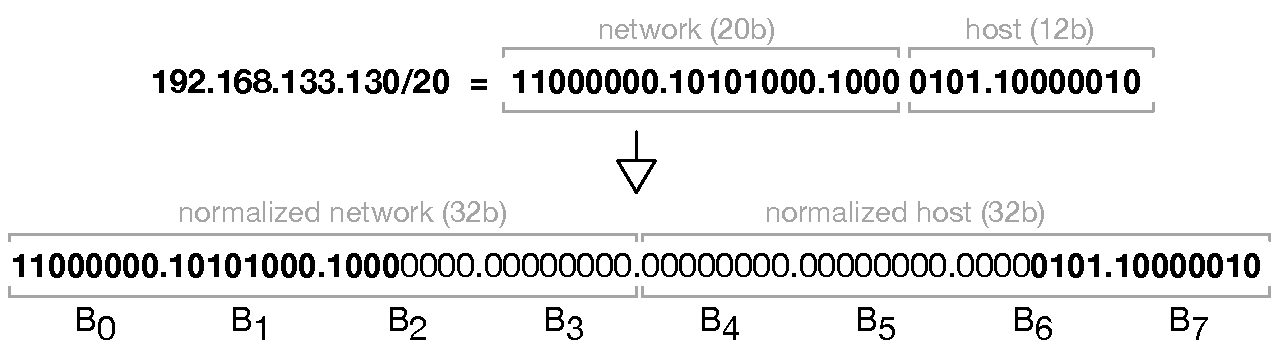
\includegraphics[width=\linewidth]{Graph/dip/normalized-ip}
	\caption{Generating a normalized IP address for 192.168.133.130/20.}
	\label{fig:normalizedip}
\end{figure}

\begin{figure*}[t]
	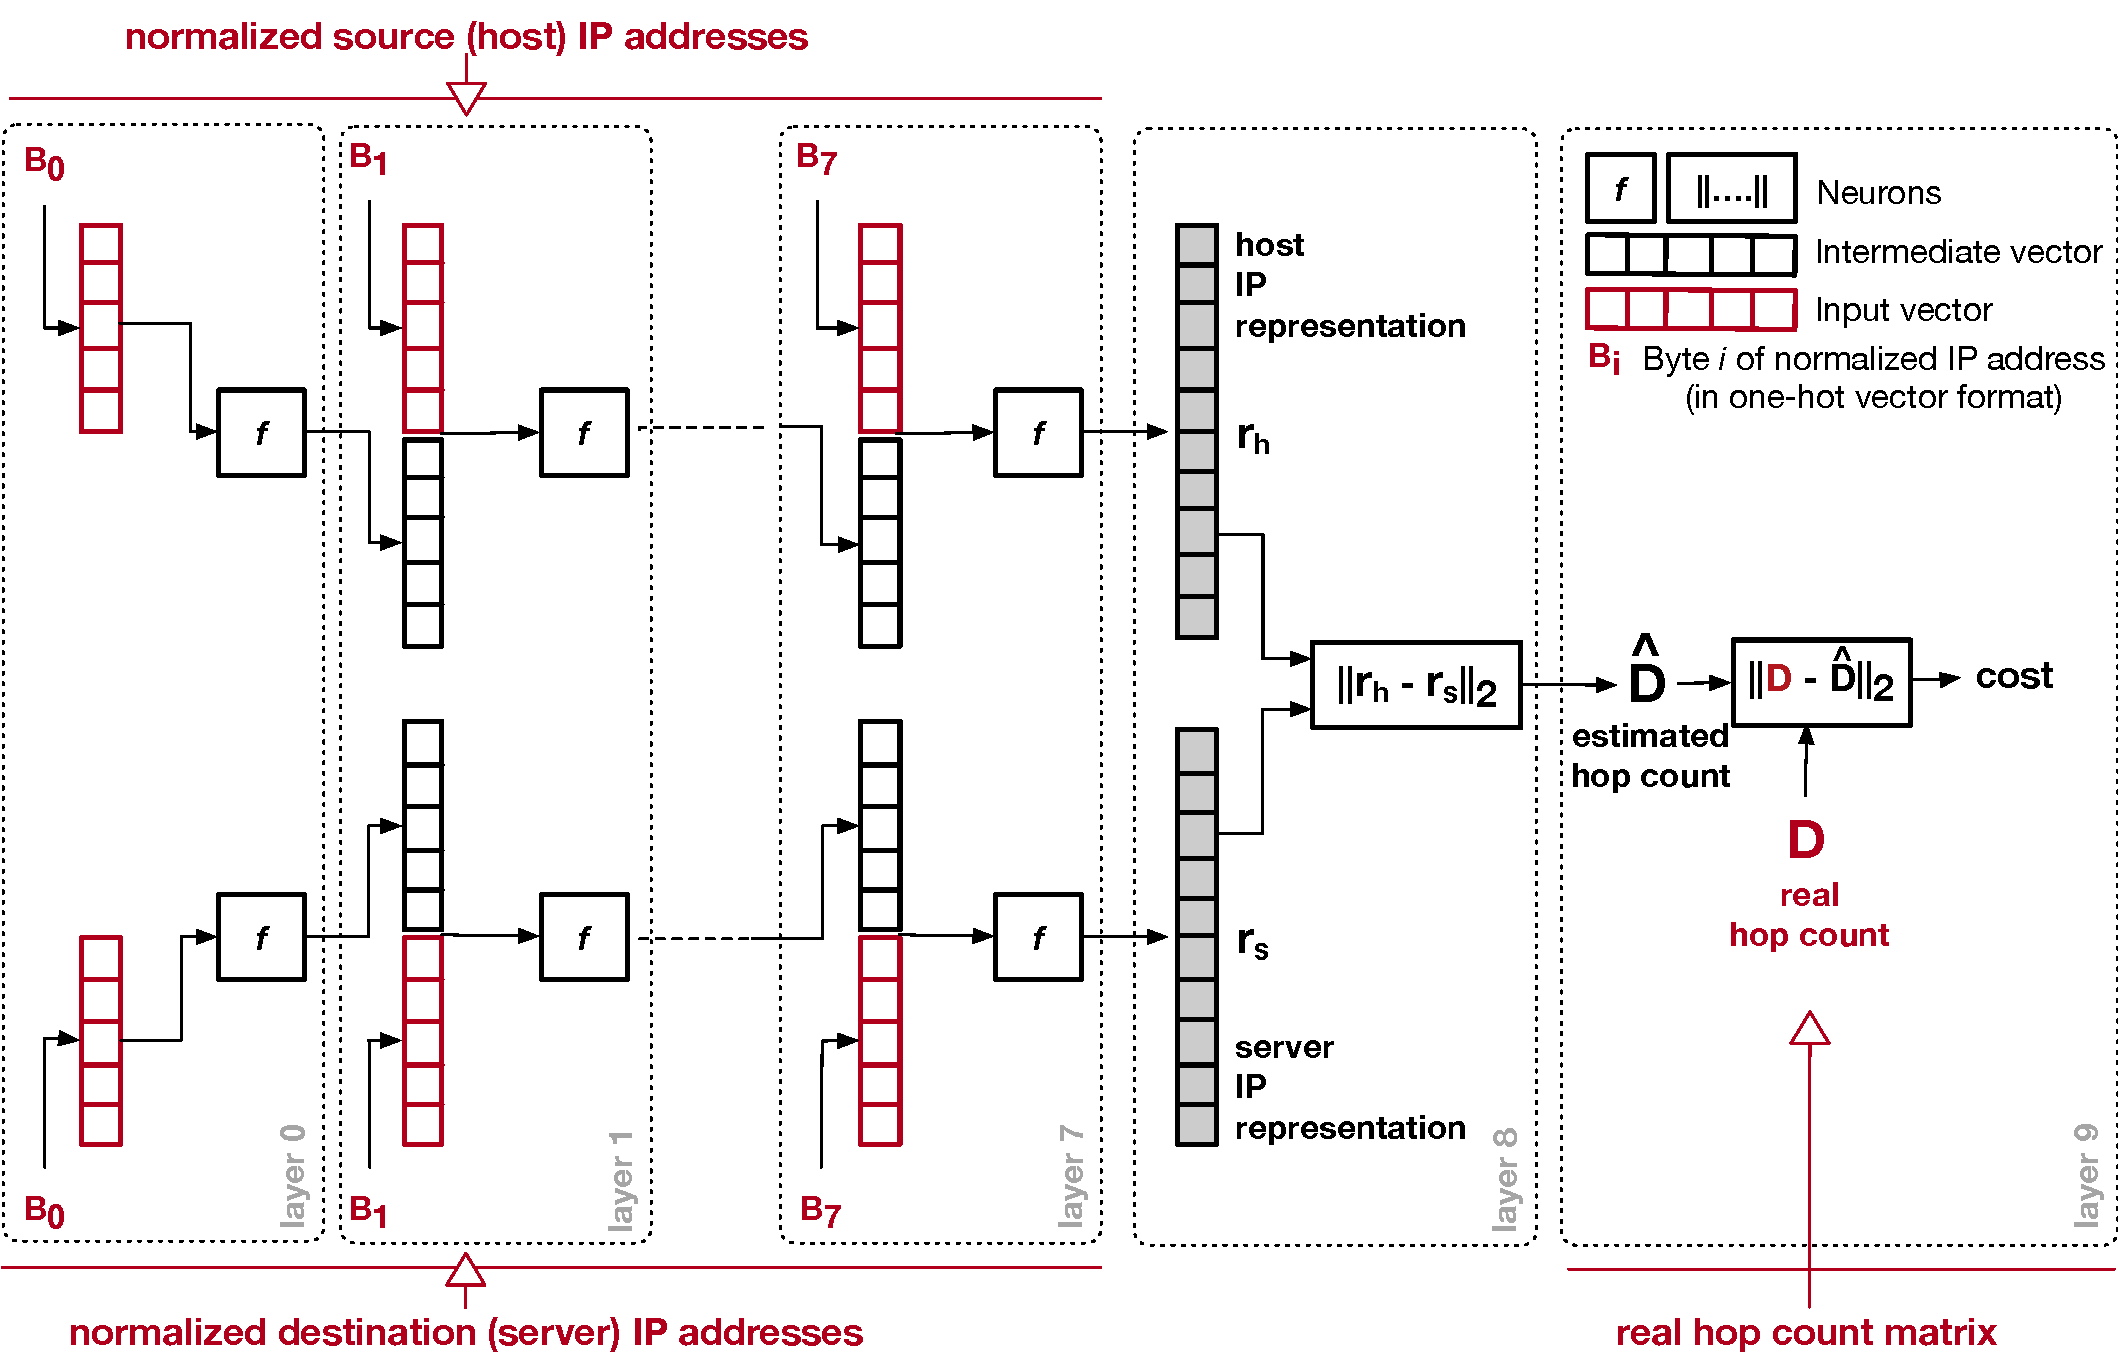
\includegraphics[width=.9\textwidth]{Graph/dip/neural-network-2}
	\caption{The neural network used for training our embedding model. The first eight layers receive the normalized IP addresses as input and compute the IP representations. The ninth layer estimates the hop count between two IP addresses and the tenth layer measures the model error. Elements in red are input. For simplicity we depict the input as one-dimensional vectors (one normalized IP); in reality, all inputs are matrices.}
	\label{fig:neuralnetwork}
\end{figure*}

As shown in Figure~\ref{fig:difference}, an IP address can help learn node representations that capture the network structure. The more bytes of an IP address we know, the better we can constrain the representation we assign to it. In addition, the more significant bytes of an IP address have a higher influence on the position of the associated host relative to other hosts. Therefore, the key is to capture the sequential correlation among the bytes of an IP address. %\mingda {This insight encourages us to borrow idea from recurrent neural networks~\citep{mikolov2010recurrent}, which take sequences of input, and processes each input conditioned on the context provided by processing the previous input (\eg{}, like processing natural language), to design our network.} 

% Previous: This insight leads to our network design: a variant of recurrent neural networks~\citep{mikolov2010recurrent}, which takes sequences of input, and processes each input conditioned on the context provided by processing the previous input (\eg{}, like processing natural language).


%\textbf{Insight:} Treat the bytes of an IP address differently inside the neural network to take advantage of the hidden structural information encoded inside an IP address.



%Decision 2: Normalize IP address to encode the routable prefix information.





%Each Source IP or Destination IP is represented by a one-hot vector. Suppose there are \textit{s} Source IPs and \textit{d} Destination IPs. Each IP address will be represented by a $(s + d)$ dimension vector. If we number each IP address from 1 to $(s + d)$, then the one-hot vector $v = \{v^1, v^2, ... ,v^{(s + d)}\} $ for the $i^{th}$ is shown as following:
%\begin{equation}    {v_{i}}^u =
% \begin{cases}
%    0   &  \text{if $u != i$ } \\
%   1    &  \text{if $u == i$}
% \end{cases}                \end{equation}
%With all the $(s + d)$ one-hot vectors, an identity matrix $m$ with size $(s + d)$ could be formed. The embedding process is shown in Figure. 

%\textbf{Hop count.} This is represented by the distances between the pairs of IPs. Because %it requires two IP addresses, we propose that at each step of the algorithm we feed the IP %address to obtain an initial representation which we refine using the distance. 

\subsubsection{Network construction}

Driven by the insight gained in the previous section, we develop \system{}, a deep neural network that computes vector representations of network hosts based on their IP addresses and the hop counts to other hosts. 
%
The design of \system{}, depicted in figure ~\ref{fig:neuralnetwork}, is similar to that of a recurrent neural network~\citep{mikolov2010recurrent}, where new data is processed in  the context provided by previous data (\eg{}, like processing natural language).
%
%Figure~\ref{fig:neuralnetwork} depicts a high-level design of \system{}. 
We explain the details below. Even though the figure and our explanation refer to the input as one-hot vectors (\eg{}, a normalized IP is represented as a vector of size 8x256=2,048), in reality the inputs are matrices (\ie{}, the number of IP addresses times 2,048). Because our hop count data (see Section~\ref{subsec:data}) is between separate end-hosts (sources) and servers (destinations) and because distances in the Internet are not always symmetric, we choose to feed the source and destination IPs separately in the neural network. %\system{} works the same when the input hop count matrix is symmetric. 

\textbf{Intermediate IP representation.} As mentioned earlier, to get the most out of the format and value of an IP address towards building a representative embedding for its host, we should treat each byte separately. The more significant bytes can provide a context for how to interpret the less significant bytes. Thus, we choose to input each byte of the normalized IP (a 256-dimension one-hot vector $B^{i\in \{0,...,7\}}_{256\times1}$) separately at each layer of the network. The input of layer $i$ is the concatenation of byte $i$ with the output of the previous layer (except for the first layer). This %\mingda{, which takes memory of preceding layers and flows previous information}:
%Suppose we want to embed each byte to dimension $d$. The output of each layer will be a vector $O^{i\in \%{1,...,8\}}_{d\times1}$. The input for each layer ($i\in \{1,...,8\}$) will be as equation \eqref{equ:input}:
\begin{align} 
\label{equ:input} 
Input=
\begin{cases}
i = 0&\parbox{.25\textwidth}{$ B^{i=0}_{256\times1}$} \\
i\in\{1,...,7\}&\parbox{.25\textwidth}{$ concat(f^{i-1}_{d\times 1},  B^{i}_{256\times1})$ } 
\end{cases}
\end{align}
where $d$ is the dimension of the final IP representation and \emph{concat} represents the vector concatenation operation.

At each layer, the activation function $f$ is given by:
%When we assign a weight $w^{i\in{\{2,...,8\}}}_{d\times(256+d) }$ ($w^{i=1}_{d\times 256 }$) and a bias $b^{i\in{1,...,8}}_{d\times1}$ for the $i^{th}$ layer, the output is represented by applying a non-linear activation function (Softsign) on the input of a layer as equation \eqref{equ:ilayer}: 
% \begin{equation} 
% \label{equ:ilayer} 
% O^{l=i}= Softsign(w^{l=i}_{d\times (256+d)}\times I^{l=i}_{(256 + d)\times 1}+b^{l=i}_{d\times1})
% \end{equation}
\begin{align} 
\label{equ:ilayer} 
f^{i}=
\begin{cases}
i = 0&\parbox{.25\textwidth}{$softsign(w^{i=0}_{d\times 256}\times B^{i=0}_{256 \times 1}+b^{i=0}_{d\times1})$} \\
\\
i\in\{1,...,7\}&\parbox{.28\textwidth}{$softsign(w^{i\in \{1,...,7\}}_{d\times (256+d)} \times concat(B^{i\in \{1,...,7\}}_{256 \times 1}, 
	f^{i-1}_{d\times 1})+b^{i\in \{1,...,7\}}_{d\times1})$ } 
\end{cases}
\end{align}
where $w^{i\in \{0,...,7\}}_{d\times (256+d)}$ are weights and $b^{i\in \{0,...,7\}}_{d\times1})$ are biases; the \emph{softsign} function is $f(x) = \frac{1}{1+|x|}$. Initially, we assign random values to all weights and zeros to all biases. We employ \emph{softsign} as the activation function for the ease of training, as \emph{softsign} is more robust to saturation compared to other popular activation functions, such as \emph{sigmoid} and \emph{tanh}. %\mingda{The weights for different layer will have different ranges. The range for the first four layers (routable layers) will be larger.												}

\textbf{Intermediate distance estimation.} We use the first eight layers of the neural network to process each of the eight bytes of the input normalized IP address. The output of the eighth layer is the intermediate vector representation for each IP address in the input data. 
%The representation is based only on the structure of an IP address. 
%The next step in the processing is to go through one more layer ($9^{th}$ layer) to improve the embedding  flexibility and accuracy in a higher dimension ($d+delta$ dimension) via adjustment of weight and bias but not normalized bytes. 
%\eqref{equ:9layer}: 
%\begin{equation} 
%\label{equ:9layer} 
%O^{i=9}= Softsign(w^{i=9}_{(d+delta)\times d}\times O^{i=8}_{d\times 1}+b^{i=9}_{(d+delta)\times1})
%\end{equation}
%Then, we could measure the error of the whole embedding in predicting the distances and refine it towards minimizing the error. 
We then use the last two layers to estimate how good the representation is.
First we compute the estimated hop counts given by the current representation using an Euclidean distance. 
%All the previous equations show the transforming for a single IP address. After applying the same transformation to all the $h$ hosts and $s$ servers, we could get 
Given two matrices $H_{h\times d}$ and $S_{s\times d}$ storing the intermediate representations for the $h$ hosts and $s$ servers separately, the estimated distance matrix is:
%\todo{Mingda: what are H and S?}Ans: Just label to distinguish the two matrices: 
%$Dist_{h\times s}$ could be described as equation \eqref{equ:distance}. The $Euclidean$ is a function created to compute the Euclidean distance of any pair of the two coordinates (rows) $r^{H_{i\in{\{1,..,h\}}}}$,  $r^{S_{i\in{\{1,..,s\}}}}$ in two matrices. 
\begin{equation} 
\label{equ:distance} 
Dist_{h\times s}=Euclidean(H_{h\times d}, S_{s\times d}) 
\end{equation}



%\todo{If I need to mention details of implementing Euclidean}

\textbf{Error reduction.} Finally, we compare the estimated hop counts with the real hop counts matrix $D_{h\times s}$ to compute the cost as the mean difference of hop-counts. 
%The goal is to minimize the difference between them. 
As the real hop count matrix is sparse, we compare only the valid entries:
\begin{equation} 
\label{equ:cost} 
Cost = \frac{\sum_{i=1}^{h} \sum_{j=1}^{s}W^{(i,j)}(||r^{H_{i\in{\{1,..,h\}}}}_{d\times1} - r^{S_{j\in{\{1,..,s\}}}}_{d\times1}|| - D^{(i,j)})}{count\, of\, non-zero\, D^{(i,j)}} 
\end{equation}
$D^{(i,j)}$ represents the value of the element at $i^{th}$ row  and $j^{th}$ column in matrix $D$. $r^{H_{i\in{\{1,..,h\}}}}_{d\times1}$ and $r^{S_{j\in{\{1,..,s\}}}}_{d\times1}$ are rows in the matrices $H_{h\times d}$ and $S_{s\times d}$, and correspond to the representation of a host or server in the embedding space. $W$ is a binary (0-1) matrix whose elements are defined as:
\begin{equation}    W^{(i,j)} =
\begin{cases}
0   &  \text{$D^{(i,j)} == 0 $} \\
1    &  \text{$D^{(i,j)} \neq 0$ } 
\end{cases}                \end{equation}
To minimize the cost, we utilize the Adam algorithm, a gradient descent based back-propagation method~\citep{kingma2014adam}, which is able to automatically tune the learning rate during the training process.


\subsection{Evaluation}
\label{dip:eval}

\subsubsection{Data and methodology}
\label{subsec:data}

We use a large data set of network hop counts from the Ark project~\citep{ark}. The data contains hop count information from 95 geographically distributed servers to ten million IP addresses that cover all routable prefixes in the Internet. We use data collected by Ark during Jun 2015. For each IP in the data, we look up the routable prefix and normalize it using the steps in Section~\ref{dip:ipnorm}.
%
Due to the cost of monitoring a large number of IPs, not all servers have hop counts for all ten million IPs. Our hop count matrix is incomplete and contains valid entries for only 29\% of the pairs. We extract IP prefix information from Routeviews data~\citep{routeviews} and use a default value of 24 for missing prefixes.


We build a prototype for \system{} using TensorFlow. We train the neural network using several smaller data sets obtained by randomly sampling 1,000, 10,000, and 100,000 IPs from the original data and keeping only the hop counts to them. Sampling increases the sparsity of the data: less than 15\% of the entries in the smaller data sets are valid. We also vary the number of servers and the dimensionality of the embedding space. Intuitively, having fewer IPs or servers may not provide sufficient constraints to learn accurate representations and lead to an underfit model. Increasing the number of dimensions can reveal more hidden features, invisible at lower dimensions, but may lead to overfitting. Each training session has 2,500 iterations, \ie{}, passes through the neural network to update the weights and biases. We use a GPU server with four 3.5GHz quad-core Intel Xeon processors and 128GB of RAM. We generate testing sets by randomly sampling the original data and preserving the previously trained parameters for embedding arbitrary IP via its address (\eg{}, the weights and biases of each byte/layer).

%We generate testing sets by sampling the orig- inal data and making sure to preserve the parameters of training (e.g., the same number of servers or IPs).

\subsubsection{Embedding accuracy}

\textbf{Clustering.} First, we assess how well \system{} preserves the clustering of hosts in the original IP space. For this, we group all IPs first according to their routable prefix and then at random. For each cluster we compute an embedding similarity metric, defined as the ratio between the average distance between all pairs of IP representations in the cluster and the maximum distance across all clusters. The lower the similarity value, the closer to each other the IPs of a cluster are in the embedding space. Figure~\ref{fig:clustering}(left) shows the similarity distribution for prefix-based and random clusters. Each IP representations is a 140-dimensional vector and computed after training the network using 10,000 IP addresses and 95 servers. Our embedding preserves the clustering of the original IP space well. 

\begin{figure*}[t]
	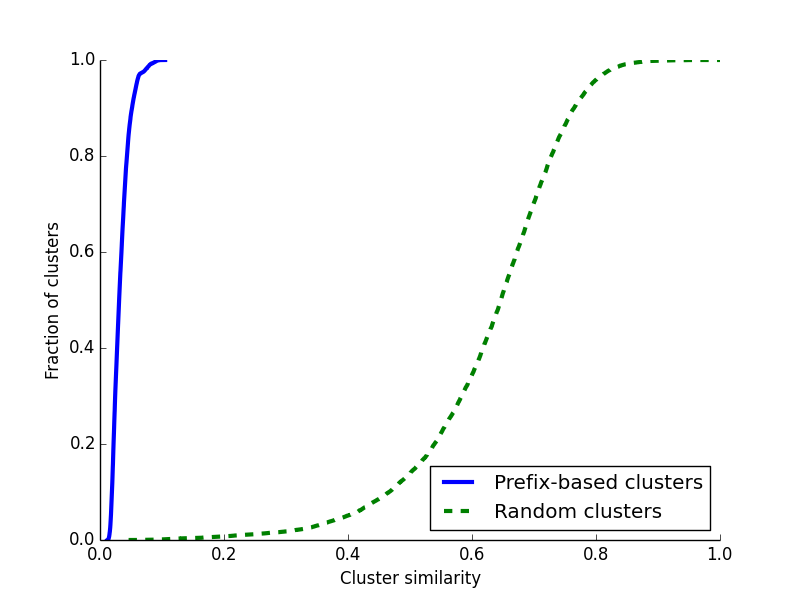
\includegraphics[width=.45\linewidth]{Graph/dip/clustering.png}
	\includegraphics[width=.45\linewidth]{Graph/dip/AbsDiffKnown12Unknown.png}
	\caption{(left) Cumulative distribution of cluster similarity, computed using IP vector representations, for prefix-based and end-host random clusters; (right) Cumulative distributions of absolute distance estimation errors for \system{}  and {\em mean}. \system{} representations preserve real-world prefix-based clustering and predict distances accurately.}
	\label{fig:clustering}
\end{figure*}

%\begin{figure}
%  \includegraphics[width=\linewidth]{AbsDiffKnown12Unknown.png}
%  \caption{Cumulative distributions of the absolute distance estimation error for \system{}  and {\em mean}.}
%  \label{fig:AbsKnown}
%\end{figure}

\textbf{Distance prediction.} To assess the quality of distance prediction, we first look at previous embedding mechanisms. Network coordinate approaches~\citep{vivaldi,gnp} are not directly comparable as they embed latencies between strategically chosen pairs of nodes, while we rely on hop count information from passively observed traffic. Eriksson~\etal{}~\citep{barford-infocom} propose a matrix factorization based algorithm to predict hop count information but first build baseline representations of the monitoring servers using an all-to-all hop count matrix. We lack complete hop count information among servers and build our embedding directly from incomplete server-to-host distances. Therefore, we compare against a {\em mean estimation approach}, where we predict a host-to-server distance as the mean of all valid distances to the same  server.

%\todo{Mingda, explain between what is the mean}
%
%\textbf{Mean estimation approach.} For the hop counts in training set between hosts and servers, we group the hop counts by servers. In each group, we calculate the mean value as the estimated hop count for the test set's same server. Meanwhile, the average value of the whole training hop counts is used  when the server in testing set is not related in training set. 


We look at how well our embedding estimates the hop count value between a host and a server. We first consider only the IP addresses used in the training process (\ie{}, {\em known IPs}). For this, we train a model using 90\% of all host-server pairs and use the remaining 10\% for testing. Figure~\ref{fig:clustering}(right) compares the absolute error between estimated and real hop count for \system{} and {\em mean} for the 10,000 IPs data set on 140 dimensions. \system{} predicts distances with a mean absolute error of around two hops (23\% mean relative error) and reduces the error of the {\em mean} estimation by almost 30\%.
%
Table~\ref{tab:abserror} presents the average absolute error and standard deviation for hop count estimation for embeddings trained with different number of hosts, servers, or dimensions. As expected, increasing the the number of IPs, servers, or the dimensionality reduces the absolute error. We also trained models with parameters outside the ranges presented in the table but found no improvement.





%\begin{figure}
%  \includegraphics[width=\linewidth]{AbsDiffKnown11Unknown.png}
%  \caption{Cumulative distributions of the absolute distance estimation error for \system{}  and {\em mean}. Log Scale}%
%  \label{fig:AbsKnown}
%\end{figure}


%\begin{figure}
%  \includegraphics[width=\linewidth]{AbsDiffKnown.png}
%  \caption{Absolute difference for known IP address}
%  \label{fig:AbsKnown}
%\end{figure}
%\begin{figure}
%  \includegraphics[width=\linewidth]{RelDiffKnown.png}
%  \caption{Relative difference for known IP address}
%  \label{fig:RelKnown}
%\end{figure}
%\begin{figure}
%  \includegraphics[width=\linewidth]{AbsDiffKnownDiffSet.png}
%  \caption{Absolute difference for various  set of servers}
%%  \label{fig:AbsKnownCluster}
%\end{figure}
%\begin{figure}
%  \includegraphics[width=\linewidth]{RelDiffKnownDiffSet.png}
%  \caption{Relative difference for various set of servers}
%  \label{fig:RelKnownCluster}
%\end{figure}
%\begin{figure}
%  \includegraphics[width=\linewidth]{AbsDiffunknown.png}
%  \caption{Absolute difference for known and unknown IP address}
%  \label{fig:Absunknown}
%\end{figure}
%\begin{figure}
%  \includegraphics[width=\linewidth]{RelDiffunknown.png}
%  \caption{Relative difference for known and unknown IP address}
%  \label{fig:Relunknown}
%\end{figure}
\iffalse
\begin{table}

		\begin{tabular}{c|c|c|c|c}
			& \textbf{\system{}} & \textbf{\system{}}& \textbf{mean} & \textbf{mean}\\
			& \textbf{known IPs} & \textbf{new IPs}& \textbf{known IPs} & \textbf{new IPs}\\
			\hline
			\multicolumn{5}{l}{\bf Number of IPs}\\
			\hline
			1,000 & 2.13690 (1.78253) & 2.88863 (2.38421) & 2.99 (2.44) & 3.27 (2.51) \\
			10,000 & 2.08812 (1.84692) & 2.71904 (2.31317) & 2.99957 (2.42138) & 3.04499 (2.43272) \\
			100,000 & abs (std) & abs (std) & abs (std) & abs (std) \\
			\hline
			\multicolumn{5}{l}{\bf Number of servers} \\
			\hline
			12 & 2.94 (2.58) & 2.95695 (2.48825) & 3.09755 (2.56616) & 2.98796 (2.55121) \\
			24 & 2.39154(2.13572) & 2.78193 (2.3314) & 2.90291 (2.36156) & 2.96651 (2.41520) \\
			48 & 2.33922 (2.04926) & 2.75361 (2.27355) & 2.99442 (2.39106) & 3.02161 (2.40399) \\
			95 & 2.08812 (1.84692) & 2.71904 (2.31317) & 2.99957 (2.42138) & 3.04499 (2.43272) \\
			\hline
			\multicolumn{5}{l}{\bf Embedding dimension} \\
			\hline
			110 & 2.27621 (1.93433) & 2.79710 (2.39204) & 2.99957 (2.42138) & 3.04499 (2.43272) \\
			140 & 2.08812 (1.84692) & 2.71904 (2.31317) & 2.99957 (2.42138) & 3.04499 (2.43272) \\
			170 & 2.18678 (1.85972) & 2.72381 (2.33045) & 2.99957 (2.42138) & 3.04499 (2.43272) \\
	\end{tabular}
	\caption{Absolute error of distance prediction when varying the number of IPs the number of servers and the embedding dimension. We show standard deviation between brackets. The default values are 10,000 IPs, 95 servers, and 140 dimensions.}
	\label{tab:abserror}
\end{table}
\fi

\begin{table}
	\centering
		\begin{tabular}{|c|c|c|c|c|}
			\multicolumn{1}{c}{} & \multicolumn{2}{c|}{\bf \system{}} & \multicolumn{2}{c}{\textbf Mean}\\
			\cline{2-5}
			\multicolumn{1}{c}{} & \textbf{known IPs} & \textbf{new IPs}& \textbf{known IPs} & \multicolumn{1}{c}{\textbf{new IPs}}\\
			\hline
			\multicolumn{5}{l}{\bf Number of IPs}\\
			\hline
			1,000 & 2.16 (1.86) & 2.89 (2.38) & 2.99 (2.44) & 3.27 (2.51) \\
			10,000 & 2.15 (1.79) & 2.68 (2.34) & 3.00 (2.40) & 3.04 (2.43) \\
			100,000 & 2.06 (1.76) & 2.29 (2.00) & 2.98 (2.40) & 2.97 (2.40) \\
			\hline
			\multicolumn{5}{l}{\bf Number of servers} \\
			\hline
			12 & 2.79 (2.25) & 3.03 (2.47) & 3.21 (2.54) & 3.28 (2.62) \\
			24 & 2.39(2.14) & 2.60 (2.25) & 2.90 (2.36) & 2.97 (2.42) \\
			48 & 2.34 (2.05) & 2.75 (2.27) & 2.99 (2.39) & 3.02 (2.40) \\
			95 & 2.15 (1.79) & 2.68 (2.34) & 3.00 (2.40) & 3.04 (2.43) \\
			\hline
			\multicolumn{5}{l}{\bf Embedding dimension} \\
			\hline
			110 & 2.28 (1.93) & 2.80 (2.39) & 3.00 (2.42) & 3.04 (2.43) \\
			140 & 2.15 (1.79) & 2.68 (2.34) & 3.00 (2.42) & 3.04 (2.43) \\
			170 & 2.19 (1.86) & 2.72 (2.33) & 3.00 (2.42) & 3.04 (2.43) \\
			\hline
	\end{tabular}
   
	\caption{Absolute mean error (standard deviation between brackets) of distance prediction of \system{} and {\em mean}, for both known and new IPs, when varying the number of IPs, the number of servers and the embedding dimension. The default values are 10,000 IPs, 95 servers, and 140 dimensions.}
	\label{tab:abserror}
\end{table}



\textbf{New IPs.} An important feature of \system{} is its ability to impute hop count values to arbitrary nodes based on their IP address. %No other embedding approach is able  use domain-knowledge based methods to estimate the hop count between IPs not used in the training process, such as the average distance between known IPs in the same AS~\citep{barford-infocom}, or gaussian mixture modeling~\citep{barford-sigcomm}. Instead, \system{} relies only on the value of the IP address and the learned embedding model without any other domain knowledge. 
{\em New IPs} are IP addresses not used in the training process and that DIP has never seen before.
% Previous: which are not included in the training set. 
Figure~\ref{fig:clustering} (right) and Table~\ref{tab:abserror} show that \system{} approximates distance to new IPs with high accuracy. The distance prediction error is only around half a hop more than that for known IPs. To the best of our knowledge, DIP is the first framework to predict hop counts to arbitrary hosts based only on the value of their IP address and routable prefix and without any other domain knowledge.
%, only . %We note that our results are similar to those obtained by Eriksson~\etal~\citep{barford-infocom} after refining matrix factorization with AS information.


%\vspace{-0.5cm}
\subsection{Discussion}
\label{dip:discussion}

We discuss several future applications and directions of using deep learning to understand and capture the Internet structure.

\textbf{Extensions.} An important benefit of using neural networks for learning the structure of the Internet is that they can be extended easily for other data sources. 
%
Similarly to previous embedding approaches~\citep{vivaldi,gnp}, we could use latency measurements instead of, or in addition to, hop counts. This would require simply changing the cost estimation part of the neural network (last two layers). While gathering latency measurements is expensive as it introduces traffic into the network, the ability of our approach to work with sparse data can limit the cost necessary to obtain the measurements. 

Furthermore, AS membership information could help find more accurate representations as many ASes cover limited areas in the network and provide a coarse indication of locality~\citep{barford-infocom}. To add AS membership information, we could either extend the shape of our input vectors (by adding two bytes for AS number) or adapt the cost estimation layers to use AS data in estimating error, similarly to Eriksson~\etal~\citep{barford-infocom}.

\textbf{Applications.} Building a model that accurately predicts structural properties of the Internet has several applications. Knowing the distance to remote IPs can help selecting a load balancing server or an overlay peer more efficiently and without having to perform expensive measurements. Understanding how nodes are clustered can make the transmission of video or large files faster by using close-by CDN nodes. 
%
\system{} can be a passive defense mechanism against IP spoofing attacks, where malicious users change the source IP of attack packets to avoid identification and subvert authentication. By comparing the predicted distance according to the spoofed source IP to the real distance (extracted from a packet's TTL field), one could verify whether the packet is spoofed or not~\citep{hc-filter}. 

%Furthermore, to find the true source of attack traffic, one could find the true representations of the real source and map it back to the IP space. We are currently working towards extending our modeling technique to offer such security services.


\textbf{Limitations and future work.}
Our current approach uses structural information embedded in the value of IP addresses, routing data, and distances between nodes, but does not consider the actual physical links between nodes on the Internet (\ie, the Internet physical topology). Adding topology would further constrain the embedding, since it is well known that the Internet is not a metric space and latency or hop count distances cannot always be embedded in metric spaces~\citep{vivaldi}. We plan to extend our framework using graph embedding algorithms to take advantage of physical topology information~\citep{dn-emb}.

While our preliminary experiments focused on accuracy, the performance of building an embedding model is equally important. Training a model with 100,000 addresses and 95 servers on our 16-core GPU server takes a few hours, indicating that we may need to train models incrementally when resources are constrained~\citep{bruzzone1999incremental}. For example, in a live deployment, we envision reconstructing our model every few days to capture the changes in topology triggered by the dynamic Internet. We are currently studying ways to incrementally add or update models without rebuilding from scratch.

Because our data is sparse, not even the best embedding may be able to recover all structural properties. While we show that our results are reasonably accurate, even when we have less than 15\% of all distances available, getting more data is clearly helpful~\citep{barford-infocom}. We plan to use active monitoring techniques (\eg{}, {\em traceroute}) to collect more information for the training phase. Knowing the IPs and connectivity of routers in the network would make the training data set richer and constrain the representation of end-hosts further.

\subsection{Conclusions}
\label{dip:conclusions}

We used deep learning to learn vector representations for nodes in the Internet based on their IP address, routing information, and a sparse hop count distance matrix. Deep learning helps uncover hidden features in the input data and recover structural properties of the Internet, such as node clusters or distances between nodes. Our experiments on a large real-world data set show that our embeddings can recover most distances, even to arbitrary hosts, with two hops absolute error, even when the training data is sparse. 
%\todo{I think it is 13\% for 10,000}



\section{Learning IP Maps for Network Spoofing Detection}
\subsection{Introduction}
\label{spoof:intro}

Spoofing the source IP address of network packets is a mechanism frequently used in denial-of-service attacks~\citep{spoofing-ddos,spoofing-ps}. IP spoofing can both hide the true source of the attack, thereby subverting IP-based firewalls and authentication mechanisms, and force legitimate hosts to redirect malicious traffic, thereby amplifying the effects of the attack~\citep{github-spoofing}. In 2018 alone, IP spoofing was the vehicle for several high-profile, terabyte-size DDoS attacks~\citep{cloudflare,github-spoofing,arbor-spoofing}.  

There are two types of defenses against spoofing attacks. Active methods encrypt connections~\citep{ipsec}, probe suspicious IPs~\citep{puzzles}, or mark legitimate packets with unique identifiers~\citep{spm,spi}. They come at the expense of bandwidth, latency, or computation overhead~\citep{ipsec-overhead}.
%
Passive (or map-based) defenses construct explicit offline maps between IPs and immutable structural network properties, such as paths~\citep{rbf,idpf}, neighboring networks~\citep{ingress,egress,rpf}, or hop counts~\citep{iphc} and filter packets whose header information does not match the maps.


Passive map-based defenses have little detection overhead and are less intrusive than active defenses, but pose a significant construction cost.
%
Measuring the network properties associated with each IP is a long and tedious process that requires intrusively probing other hosts, querying routing tables, or passively waiting to receive sufficient traffic~\citep{hcf}.
%
In addition, as network properties are different for every vantage point, maps computed for a location cannot be easily transferred to a different location and must be recomputed.

We propose to {\em learn a structural model (or embedding) of the Internet and use the model to predict, rather than explicitly compute, IP maps}. Learning instead of measuring network properties could significantly reduce the cost of achieving complete host IP maps while making them more general. First, training a network embedding requires only a small set of ground truth information, such as distances between IPs (\eg{}, hop counts, latencies)~\citep{vivaldi,peerwise,barford-infocom}. This reduces the amount of data necessary {\em a priori} for constructing a good map, thereby reducing the construction cost. Second, network embeddings are general and can be used to predict associations between {\em any} IP and its local network properties, even when the IP was not part of the training. %However, because many of the IP associations are learned, not measured, they may not be accurate. Learned maps may lead to less precise detection, which makes them less practical.


%. The maps are placed on AS border routers inside the network~\citep{rbf,idpf,ingress,egress,rpf} (network-based detection) or on servers at the edge~\citep{iphc} (host-based detection) and filter incoming packets whose header information does not match the maps.









%
%Building end-host maps may complement in-network spoofing mechanisms but are specific to the host on which they are constructed and difficult, if not impossible to transfer to another host.

%In this chapter, we ask the following question: how can we efficiently increase the coverage of host-based spoofing to protect {\em any} server in the Internet against attack packets spoofed with {\em any} IP address? 
%
%We identify two key contributors for the incomplete coverage of existing host-based defenses: the construction cost and specificity of IP maps.
%
%Computing the network properties associated with each IP is a long and tedious process that requires intrusively probing other hosts, querying routing tables, or passively waiting to receive sufficient traffic~\citep{hcf}.
%



%
%With {\em learned maps}, hosts do not need to compute and maintain exact mappings and could predict the associations that they do not have. In addition, a model of the Internet is general and could be used to predict maps at every host.

We study the feasibility of using network embeddings to learn IP maps for spoofing detection. Towards this goal, we present and build a learning-based spoofing detector that combines DIP, our previous deep learning based network embedding algorithm~\citep{dip,dip-ccr} and hop count filtering, and a popular host-based spoofing detection mechanism~\citep{hcf}. Hop count filtering compares the hop count information of packets arriving at a target server to the known hop count value from the packets' IP source to the target. It considers a packet spoofed if the two values do not match. 
%
Rather than build an explicit map of known IP-to-hop-count associations, we use DIP to learn a network embedding that preserves hop count distance between IPs. Using the embedding, we predict with high accuracy the hop count between any two IPs and identify when a packet is spoofed.

We analyze the coverage, accuracy, and cost of our learning-based detector. We show that learning, instead of explicitly computing IP maps, dramatically increases the detection coverage over spoofed sources and targets. Our learning-based detector needs hop count information from only around 1,000 IPs to several targets to build a model that can help detect spoofing from most of the Internet. Although, not as accurate as the original hop count filtering in detecting packets spoofed with previously known IPs (\ie{}, to which the hop count is known), ours is the first map-based detector to identify spoofing with unknown IPs (\ie{}, for which the hop count to the target is not known). It can also be used to detect spoofing to new targets, not part of the training process, with only a small loss in accuracy. In addition, learning an embedding is fast: even with almost three million hop counts from 100,000 IPs, it takes less than an hour to learn an embedding that can predict maps for any IP address.

This work brings two contributions. First, we introduce a framework to help {\em any} Internet server detect packets spoofed with {\em any} IP address without any additional measurements to that IP. This represents a major shift from previous map-based spoofing detection mechanisms, who are either restricted to specific targets or to detect packets spoofed with known IPs. Although our method does not yet achieve by itself the accuracy necessary for a real-world deployment, it nevertheless shows that learning, rather than measuring, network properties could be an important piece in the spoofing detection puzzle.

Second, our work explores the impact of deep learning in the network and security operations decision making. As AI moves beyond just being the word {\em du jour} and increasingly becomes an integral part of the network~\citep{dls}, it is important to understand the trade-offs between its cost and benefits~\citep{vern}.
%
It is precisely such a trade-off that we analyze in our work: while learning IP maps for spoofing detection can ease the task of administrators and help build complete maps much faster, it may decrease the detection accuracy. Understanding this balance can lead to better and more protected networks.

%The rest of the chapter flows as follows. In the next section, we revisit map-based spoofing detection mechanisms and reiterate the motivation for learning maps. We describe our vision for a learning-based spoofing detector in Section~\ref{sec:design}. In Section~\ref{sec:eval}, we use real world data to evaluate the trade-offs involved in introducing learning to spoofing detection. We discuss the limitations and opportunities of our work in Section~\ref{sec:discussion} and conclude in Section~\ref{sec:conclusions}.

\subsection{Towards learned maps for spoofing detection}

%Internet hosts can {\em actively} protect themselves from IP spoofing by securing their connections using private keys~\citep{ipsec}, probing suspicious IPs to check their validity~\citep{xxx}, or asking sources to send the solution to a computational puzzle before connecting~\citep{puzzles}. All these solutions are expensive to deploy and may introduce performance overhead in the form of additional network throughput and latency~\citep{ipsec-overhead}.

Map-based spoofing defense mechanisms associate IP addresses with immutable network properties that are difficult to modify by attackers. Packets that carry information (\ie{}, in headers) not matching the map are dropped. Unlike active spoofing defense methods that encrypt connections~\citep{ipsec} or probe suspicious IPs~\citep{puzzles}, map-based approaches are less intrusive and do not introduce additional traffic.
%
To be effective, map-based detection must provide {\em coverage}: given a random attacker, protect any target against attack packets spoofed with any IP address.
%

\textbf{Network maps.}
Network-based maps reside on AS border routers and pair IPs to the incoming network interface~\citep{rpf,idpf} or with keys inserted in the packet by an upstream trusted party~\citep{spm}. Such maps have the potential to provide complete coverage, if installed pervasively by {\em all} ASes. However, their deployment has been slow. Recent measurements performed by CAIDA~\citep{spoofing-state} show that around 25\% of all ASes allow spoofed traffic to traverse them. Until all networks deploy network-based detection, the Internet is susceptible to spoofing.
%
A likely cause for the incomplete coverage is the misaligned economic incentives~\citep{pam17-loops}: the cost to deploy network maps is high and supported by each AS, while the benefit is incremental and spread to the entire Internet.


%
%Host-based detection aligns the incentives by pushing the detection to the edge: hosts are responsible for building their own maps and benefit immediately from them. However, this comes at the expense of decreased coverage: detection benefits only the host of the map and is limited to packets spoofed with IPs present in the host's map.



\textbf{Host maps.}
Host-based detection aligns the incentives by pushing the onus of detection towards the edge of the network. Hosts\footnote{Throughout the chapter, we interchangeably refer to the server that deploys host-based maps as host, end-host, target, destination, or victim.}, rather than routers, build and maintain IP maps and benefit immediately from them. Most notably, several solutions build maps between IPs and hop count values to the target, relying on hop count data as a measure of the network topology~\citep{iphc,hcf}. 
Hop counts can be easily derived from the IP TTL field, whose value depends on the network infrastructure (\ie{}, every router decrements the value before forwarding the packet) and cannot be easily forged by an attacker.  

By pushing map computation to the edge, host-based maps decentralize the spoofing detection process and may see decreased coverage. 
%Host map-based mechanisms have several drawbacks that could limit their detection ability. 
First, their {\em detection is limited} to packets spoofed with IPs to which the target knows the hop count. They fail in detecting packets spoofed with IPs unknown\footnote{We consider an IP address {\em unknown} to a target if the target does not know the hop count to it. Existing host-based maps cannot detect packets spoofed with an unknown IP address.} to the target. As attackers rely on surprise and obfuscation, they often use random spoofed addresses that can be from anywhere, even from non-routable
ranges~\citep{cloudflare}. Increasing coverage by building complete maps is difficult. Passively collecting hop counts from incoming traffic is not likely to provide a large coverage~\citep{hcf}, while actively probing all IPs is expensive, intrusive, and time-consuming~\citep{ark}. 
%
Second, host maps are {\em location specific}. A map associating IPs with hop counts to a target is only useful for that target and cannot be transferred to other hosts, even if they are part of the same network.
%
%Finally, unlike many structural Internet properties, maps are {\em static}. They need to be updated when paths, routes, or hop counts change. Thus, spoofing detection needs to continually monitor path changes and update maps to reflect the current state.


\textbf{Learned host maps.}
We propose to {\em learn} IP-to-hop-count mappings, instead of extracting them from incoming packets. 
%Using a limited set of IPs and hop count information, we generate a structural model of the Internet that, given any two IP addresses, can estimate the hop count between them. Learning maps can increase host-based spoofing detection (because we can estimate hop counts to any IP) and make it more general (because our model does not depend on location). 
%How can we learn a structural model of the Internet that predicts hop counts between IPs? 
A natural solution is to first learn representations of IPs in a vector space and then estimate the distance (\ie{}, hop count) between IPs as the distance between their representations. Network embedding methods can easily compute IP representations in Euclidean spaces from a limited set of latency or hop count information~\citep{vivaldi,gnp,pic,pyxida,barford-infocom}. 
%
However, they are limited to the hosts part of the training set and cannot generate representations or hop counts for other hosts. This means that they cannot be used to estimate hop counts for, and thereby detect packets spoofed with, IP addresses unknown to a target.
%perform optimizations on few, strategic measurements or passive observations to learn vector representations. Oftentimes, this is not sufficient; they resort to out-of-band information, such as location~\citep{vivaldi} or routing~\citep{barford-infocom} data, or perform active measurements~\citep{barford-sigcomm} to impute the missing data and detect clusters or distances.

The emergence of learning frameworks that preserve structural network properties such as distances or clustering among nodes offers an alternative to build explicit host-based IP maps from passive or active measurements~\citep{dip,net-emb}. 
%
Deep learning based embeddings use several data sets, \ie, distances, routing information and host IP values, to learn IP representations. Because they learn hidden structural features encoded in a node's IP address, they could generate representations for any node, given only its IP address~\citep{dip}. In addition, deep learning algorithms are easily extensible and adaptable when new or updated data is available. 

%Deep neural networks consist of multiple layers of interconnected neurons~\citep{lecun2015deep}. A neuron aggregates multiple input values using local weights and biases, applies an activation function, and produces one or more numerical values as output. 
%
%Given a training task, one can define an objective function to evaluate the output of the entire neural network, \eg{}, prediction error. 
%
%Using gradient-based back-propagation algorithms to optimize the objective function~\citep{kingma2014adam}, neural networks automatically tune the weights and biases of each neuron to archive better performance.

Figure~\ref{fig:learnedmaps} presents a visual representation of the benefits of learning-based spoofing detection. Unlike network maps, which detect only spoofed packets traversing protected ASes (left diagram), or explicit host maps, which detect only packets spoofed with IP sources known by the host (middle diagram), learned host maps can detect packets spoofed with unknown IPs (right diagram). The host uses a learned structural model of the Internet to estimate a specific network property, \eg{} hop count information, associated with the source IP of an incoming packet and decide whether the packet is spoofed or not. In the next section, we describe a learning-based spoofing detector combining hop count filtering with the DIP network embedding framework.


\begin{figure}
	\centering
	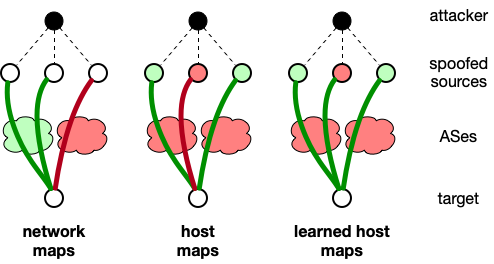
\includegraphics[width=.8\linewidth]{Graph/spoof/learnedmaps.png}
	\caption{Map-based spoofing detection. Network maps detect only spoofed packets traversing protected ASes (colored in green). Host maps detect only packets spoofed with IPs present in the map (also colored in green). Learned host maps have the ability to detect all packets because they learn missing map entries. The paths in the diagrams indicate the apparent source of the packet (the spoofed source). In reality, all packets originate from the attacker.}
	\label{fig:learnedmaps}
	\vspace{0.5cm}
\end{figure}

\subsection{Learning-based spoofing detection}
\label{spoof:design}

To illustrate the benefits of a learning-based spoofing detector, we propose a prototype detection framework based on the hop count filtering method first introduced by Wang~\etal{}~\citep{hcf}.
Our prototype consists of two main components: an offline IP map learning module (to learn IP representations and estimate hop counts between IPs) and a spoofing detector (to detect spoofed traffic). We describe both modules next and study their effectiveness in the next section. 
%Building a real spoofing detection framework is a non goal of the chapter. We merely seek to understand whether a learning-based spoofing detector is a viable direction through real-world measurements.



\subsubsection{IP map learning}

In a previous work, we introduced DIP, a deep learning framework that uses hop count information between network host to learn an embedding of the Internet~\citep{dip}. Using a small data set of IP addresses, their prefix information, and hop counts among them, DIP computes a vector representation of each IP in a high-dimensional Euclidean space. The algorithm ensures that representations reflect hop counts between hosts: the Euclidean distance between two representations estimates the hop count between the associated IPs. We briefly describe DIP below and refer the reader to the work of ~\citet{dip, dip-ccr} for more details.


The training data for DIP includes the IP addresses and hop counts among them. The IP addresses are hierarchical sequences which contain two parts, i.e. network (routable, routing prefix) and host (local) part. For example, for a 32-bit IPv4 address 192.167.2.17/24, the number 24 means the first 24 bits form the routable prefix, which can indicate the identification of the subnet. The rest 8 bits will be the local information for this IP address within the subnet. The hop count between two IPs represents the total number of intermediate devices (e.g. routers) that a data package needs to pass. We use it as the distance between two IPs and the training objective is to estimate the hop count between two IPs. The utilized hop count matrix is actually very sparse and asymmetric. During training, we will not pre-filling any value to the matrix to avoid introducing noises. We will  measure the loss only when the hop count information exists. 

The DIP is designed to exploit the above mentioned information efficiently with a variant of recurrent neural networks to capture the structure encoded in the value of an IP address (\ie{}, network part and host part provide an implicit hierarchy of IPs). According to the definition of the network and host part, we can find it is actually more significant to use the network part expressing the structural position. However, for IP addresses, their network parts can have different sizes. The network part's size can be any value from 0 to 32 (IPv4).  Similarly, the number of bits contained in the host part varies. Hence, before feeding in the IP addresses, we will normalize them by: 1) Divide the 32 bits into network and host parts; 2) For the $n$ bits in network parts, we pad in $32-n$ 0s at the end; 3) For the $32-n$ bits in the host parts, we pad in $n$ 0s at the beginning. Then, we can get two four-byte normalized values.  

With the two four-byte values, we can convert their each byte's numerical value to a one-hot vector (256 dimensions). The reason to use one-hot vector is we think there is no relationship like natural ordering or neighboring between different values of byte. For example, there are three hosts with the second byte equalling 156, 192, 15. We cannot easily say that the first two hosts are nearer to each other compared to the third because the difference between 156 and 192 is smaller. So we would like to regard the byte value as categorical data and use one-hot vector to represent. 

By two experiments result shown in Figure 1 of \citet{dip}, we  find the more bytes for an IP address, the better we can constrain the representation of the IP. This shows the sequential information contained by the IP addresses.  So, in each layer of DIP, we feed the one-hot vector of the eight bytes from the  normalized IP separately and use the structure similar to Recurrent Neural Network to capture the sequential information. Suppose the 8 bytes are $B_i, i \in {0, ..., 7}$, where each $B$ is actually converted to a one-hot vector of 256 dimensions. The input for the first layer of DIP will be $B_0$. Via  the formula:
\begin{align} 
h_{0}=activate(W_0 \times B_0 + bias_0)
\end{align}
we can get the hidden output of the first layer. The activate function can be either $softsign$, $tanh$ or $sigmoid$. In our experiments, we use $softsign$ for an easy and efficient training.

Then, for the following layers, the hidden output of the last layer will participate into the input of the current layer. 
\begin{align} 
h_{i}=activate(W_i \times [B_i, h_{i-1}] + bias_i), i \in {1, .. , 7} 
\end{align}
The $[B_i, h_{i-1}]$ means to concatenate the current input and the last hidden state. 
Then, by the $h_7$, we can add another feedforward layer to convert the $h_7$ to $h_8$ and estimate the hop count by:
\begin{align} 
hop-count = Euclidean (h_{8,source}, h_{8, destination}),
\end{align}
which utilizes the source and destination IPs' hidden representation for estimation. During learning, the trainable parameters include the $W_i$, $bias_i$ where $i\in {0,...,7}$ and the final layer's parameters to convert $h_7$ to $h_8$. Since we think the first 4 bytes, which is the normalized network part of the IP address, are more significant for structural information. We will assign a higher initial value for the $W_i$ when $i\in {0,...,3}$ and a smaller value for the $W_i$ when $i \in {4,..,7}$. This will enhance the influence of the first four layers and weaken the influence of the second four layers. The learning will be supervised: at each iteration of the algorithm, the representations are refined towards minimizing the error between estimated hop counts (computed from the Euclidean distance between two representations) and real hop counts. 
All the previous mentioned formulas and steps are simplified version for the processes described in \citet{dip}. If you need more detailed information, please check the \citet{dip}. 

% DIP uses a variant of recurrent neural networks to capture the structure encoded in the value of an IP address (\ie{}, network part and host part provide an implicit hierarchy of IPs). To allow the most significant bits of an IP (\eg{}, the network part) to influence the final representation more than the least significant bits (\eg{}, the host part), DIP feeds the bytes of an IP address sequentially. DIP's learning is supervised: at each iteration of the algorithm, the representations are refined towards minimizing the error between estimated hop counts (computed from the Euclidean distance between two representations) and real hop counts.



The advantage of DIP compared to traditional network embedding approaches is that it incorporates structural information encoded in the value of an IP address towards learning their position in a vector space. Learning from the value of an IP address is critical for our purpose. The learned model can be used to generate representations for {\em any IP}, even if it was not part of the training set or we do not have distance information to it. This, in turn, increases the coverage of our spoofing detection. We are not limited to the information from IP maps anymore; missing associations between IPs and hop counts can be easily estimated from the learned model. In addition, embedding models are general: they can be transferred to and immediately used by other hosts, without additional retraining, thereby reducing the overall cost of achieving global detection.

Notwithstanding its advantages, DIP suffers from the same limitation as previous network embedding methods~\citep{vivaldi,gnp,pic,pyxida,barford-infocom}: Internet hop counts do not form a metric space (\eg{}, they violate the triangle inequality~\citep{peerwise}) and cannot be embedded accurately into an Euclidean space. DIP is able to predict distances between Internet nodes with a mean absolute error of 2.06 hops, after being trained on distances between around 15,000 pairs of nodes. The error increase is small (from 2.06 hops to 2.29 hops) when we consider distances to IPs not used in the training, and therefore unknown to the targets. 
%
Detecting spoofed packets based on imprecise hop count information may lead to incorrect decisions. To minimize the number of missed spoofed packets, we must allow a margin of error when comparing the estimated and real hop counts. 
%
In Section~\ref{spoof:eval}, we show that spoofing detection still works when the hop count estimations are not exact and discuss how to select the detection threshold.

\begin{figure*}[t]
	\centering
	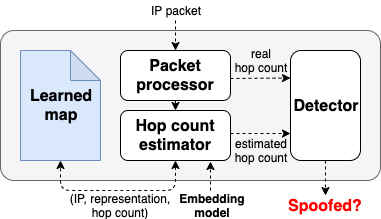
\includegraphics[width=.6\linewidth]{Graph/spoof/spoofing-detector.png}
	\caption{The learning-based spoofing detector uses an embedding of the Internet to estimate hop count information to any IP address and detect when the IP is used as the spoofed source of an attack packet.}
	\label{fig:detector}
	% \vspace{-0.5cm}
\end{figure*}

\subsubsection{Spoofing detector}

The spoofing detector is deployed on a potential target and consists of the learned map, packet processor, hop count extractor, and detector (Figure~\ref{fig:detector}). The packet processor extracts the source IP and TTL values from an incoming packet. It then computes the hop count information from the TTL, using the algorithm described by Wang~\etal{}~\citep{iphc}. The hop count estimator uses an existing embedding model (\ie{}, built offline using IP and hop count data from legitimate packets) to compute a representation for the packet's source IP and estimate the hop count to the target. 
%
The detector compares the real and estimated hop counts to the target. If the difference between them is greater that a pre-specified threshold, we consider the packet spoofed and raise an alert.
%
To save future computation, all estimated hop counts and IP representations are saved into a cached learned map. When packets from an IP present in the map arrive at the target, we use information from the map without recomputing the hop count value.



\subsection{Evaluation}
\label{spoof:eval}

We evaluate the feasibility of learning-based spoofing detection as follows. First, we analyze what coverage we can achieve compared to detectors based on exact maps, such as hop count filtering. Second, we simulate spoofing and measure how well we detect spoofed packets under various scenarios. Finally, we look at the cost of building a detector. Table~\ref{tab:spoofing} contains a summary of our findings.

\def\arraystretch{1.5}
\setlength{\tabcolsep}{5pt}
\begin{table}[t]
	\centering
	\begin{tabular}{m{.16\linewidth}|p{.75\linewidth}}
		{\bf Method} & {\bf Description}\\
		\hline
		{\bf network maps} &  Complete coverage if all ASes deploy network maps; currently 25\% of ASes are unprotected~\citep{spoofing-state}; cost of building maps is high~\citep{pam17-loops}.\\
		\hline
		{\bf host maps} & Coverage limited to the IPs with known hop count to the host: potentially covering packets spoofed with 95\% of all IPs~\citep{hcf}, if map contains {\em all} IP addresses; maps cannot be transferred and need to be explicitly computed by each host; cost of building maps is high~\citep{hcf,ark}.\\
		\hline
		{\bf learned host maps} & Limited by the accuracy of embedding; covering packets spoofed with around 70\% of all IPs, even when the IP is unknown to the host; embedding models can be transferred and do not need to retrained; cost of building maps is low.\\
		%\hline
	\end{tabular}
	\caption{Map-based spoofing detection methods.}
	\label{tab:spoofing}
	% \vspace{-0.5cm}
\end{table}


{\bf Data.} We use a large data set of network hop counts collected by the Ark project~\citep{ark} during June 2015. The data contains hop count information from 96 geographically distributed servers to ten million IP addresses that cover all routable prefixes in the Internet. 
%
Because monitoring a large number of IPs is costly, not all servers have hop counts for all ten million IPs. Our hop count matrix is incomplete and contains entries for only 29\% of the pairs.
%
Furthermore, due to privacy issues, the last eight bits of each IP were zeroed out after collection. Although this makes the set of possible spoofed sources more general, it also helps us learn more robust models, as there are likely more servers monitoring the same /24 prefix than the same single IP address, \ie{}, the number of hop counts per IP is higher. 

It is possible that the hop counts collected by Ark are to routers on the path, rather than the end host itself. This can happen when routers, and not the target, reply to the monitoring packets. As our detection algorithm is intended for the edge of the network, training with router IPs and hop counts may bias the results. It is difficult to determine precisely which response comes from a router. To minimize the potential bias, we use a simple heuristic based on the fact that many router IPs are not part of advertised BGP prefixes. Using this heuristic, we filter out around 1.2\% of the IPs in our data.
%For each IP in the data, we extract prefix information from Routeviews~\citep{routeviews} and use a default value of 24 for missing prefixes.
%




{\bf Methodology.} We build a prototype spoofing detector using TensorFlow and Python, reimplementing the learning in DIP~\citep{dip} and hop count filtering~\citep{hcf}. We train the neural network offline using several smaller data sets obtained by randomly sampling 1,000, 10,000, and 100,000 IPs from the original data and keeping only the hop counts to them. Sampling increases the sparsity of the data: less than 15\% of the entries in the smaller data sets are valid. 
%
%We use the same training parameters as described by Li~\etal{}~\citep{dip}
%
%Li~\etal{}~\citep{dip} show that increasing the size of the training set and the dimensionality of the embedding space can increase the accuracy of hop count estimation.
%
We train our spoofing detector for 1,000 iterations on a server with four 3.5GHz quad-core Intel Xeon processors and 128GB of RAM.
%




{\bf Assumptions.} We assume a single attacker, randomly placed in the Internet, with no knowledge about network structure around the spoofing target or the spoofed IP. This means that the attacker cannot use information about hop count to the target to avoid detection. We also assume that the hop count information is static and does not change. In Section~\ref{spoof:discussion}, we discuss what happens when we relax these assumptions. 

{\bf Goals and non-goals.} Our main goal is to evaluate the feasibility of learned maps for detecting spoofed network packets and to inform future decisions of security operators or researchers. We use an existing embedding algorithm, DIP~\citep{dip} to learn hop count information between IPs, and study its interaction with hop count filtering~\citep{hcf}. A non-goal is to evaluate the DIP embedding accuracy. For a detailed study, we refer the reader to the DIP chapter~\citep{dip}, which analyzes the embedding accuracy when varying various learning parameters and in contrast to other distance prediction mechanisms.
%Our focus is thus on understanding the coverage of a learning-based spoofing detector: how likely is it to protect {\em any} target from packets spoofed with {\em any} IP address. 
\begin{figure*}[t]
	\centering
	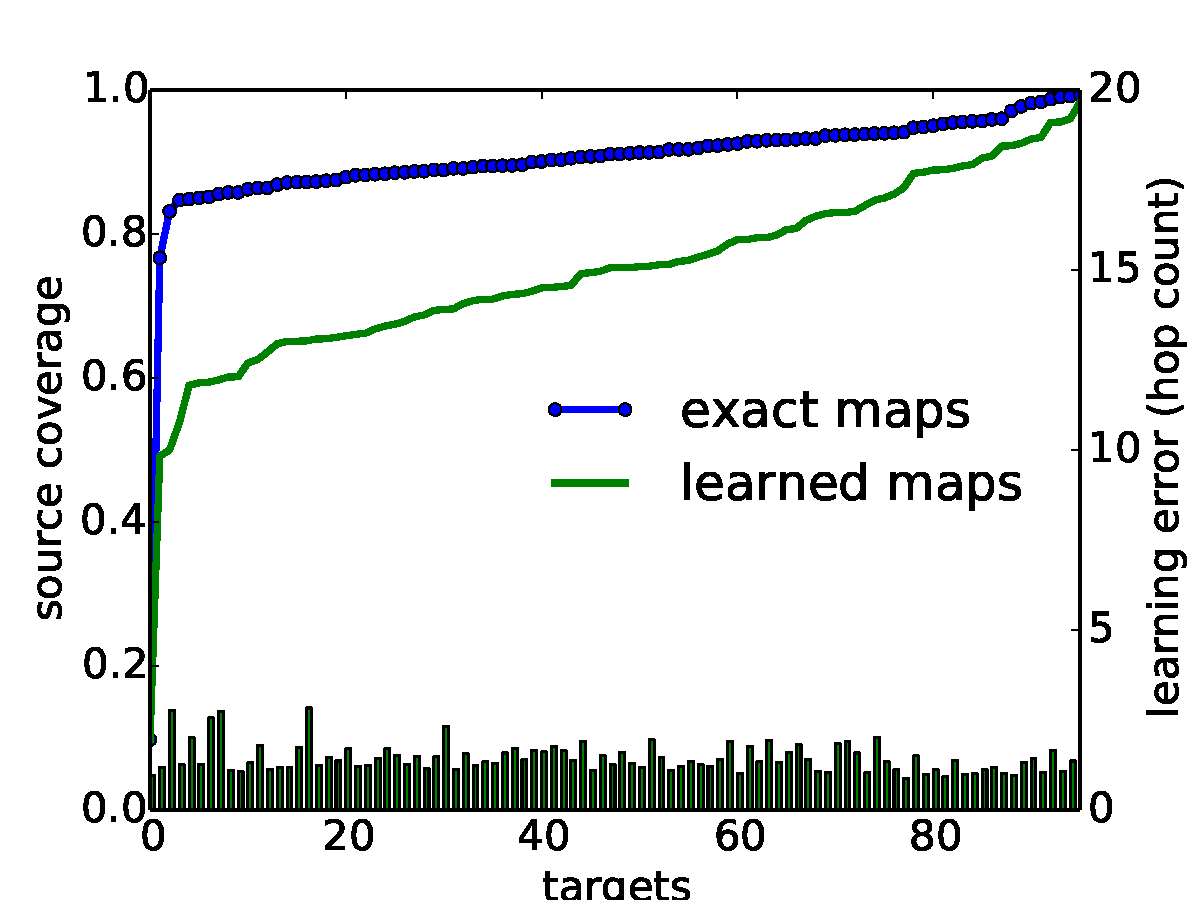
\includegraphics[width=.49\linewidth]{Graph/spoof/upperbound-upperbound-caida-jun2015-source-to-monitor-ttls-2000files-sample1000.pdf}
	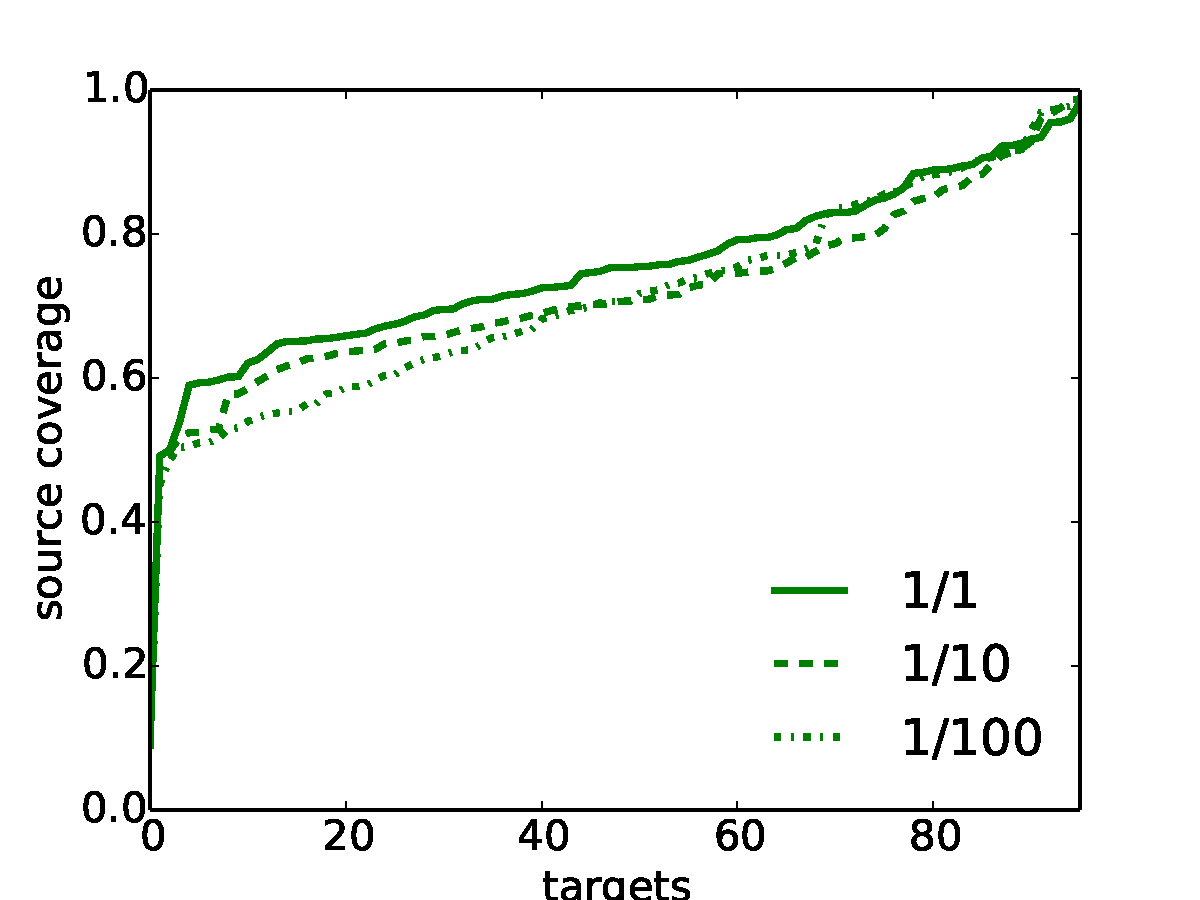
\includegraphics[width=.49\linewidth]{Graph/spoof/coverage.pdf}
	\caption{Coverage for (left) exact and learned maps for 1,000 source IP addresses, and (right) learned maps for the same sources used in training (labeled ``1/1''), ten times as many sources (``1/10''), and a hundred times as many sources (``1/100''). The bars represent the error of a learning-based spoofing detector, for each target, in hop counts. Learning-based spoofing detectors adapt well to new sources with little loss of coverage.}
	\label{fig:upperbound}
	\vspace{0.5cm}
\end{figure*}

\subsubsection{Coverage}

The limited range of hop count values (\ie{}, 0 to 255) means that no hop-count-based spoofing detector can achieve perfect detection. To understand the limits of detection, we define the {\em coverage} of each target as the expected fraction of source IPs that can be unambiguously identified when spoofed by a random attacker. In other words, the coverage represents the probability that a packet spoofed with a random IP by a random attacker is detected by the target.

{\bf Exact maps.} Before studying learning-based maps, we analyze the boundaries of what exact hop count based maps can achieve. Hop count filtering~\citep{hcf} identifies packets as spoofed when the packet hop count does not match the known hop count associated with the source address. If the attacker spoofs a packet with an IP address that has the same hop count to the target as the attacker IP, hop count filtering cannot detect the attack. 
%
To compute the coverage of exact maps, we repeatedly select a source IP at random as the attacker for each target, calculate the fraction of IPs that share the same hop count to the target as the attacker and subtract the value from 1.
%
Figure~\ref{fig:upperbound}(left) shows the distribution of coverage for all targets in our data set. We consider 1,000 IPs; results for other data sets are similar. Focus only on the line labeled {\em exact maps} for now. Most targets have a coverage of at least 0.8.

An important observation is that exact maps are not necessarily limited to detecting traffic spoofed with IPs that have communicated with the target in the past. They are efficient in detecting attacks spoofed with any IP, as long as the target knows the hop count to the IP. Oftentimes, IPs that are part of the same prefix, especially for smaller prefixes, share the same hop count to a target. Our data set already contains at most one IP per /24 prefix to ensure it does not underestimate the performance of exact maps.

{\bf Learned maps.} As described in Section~\ref{spoof:design}, learning maps introduces errors in estimating hop count values. Any learning-based spoofing detector needs to account for those errors in identifying spoofing. 
%
First, for each target, we compute the average error between real and estimated hop counts from all sources to the target. We use hop counts from 1,000 IPs to the 96 servers to learn the embedding. 
%Our training set is the same as the size of the exact maps above. 
Then, similarly to above, we select an IP at random from the 1,000 IPs in the training set as the attacker and compute the fraction of IPs whose hop count is within the estimation error of the hop count from attacker to target. We subtract this value from 1 to obtain the coverage for the learned map of each target. This captures the probability that learned maps detect packets spoofed with a random IP from a random attacker. Note that here we select an IP {\em from the training set} as the attacker to compute source coverage for known IPs and compare with exact maps. Below, we re-do the analysis for unknown IPs, that are not from the training set.
%
Figure~\ref{fig:upperbound}(left) shows that the coverage of learned maps is lower than that of exact maps when considering the same set of source IPs. On the average, a target could detect spoofed packets only 70\% of the time, compared to 90\% of the time with exact maps.

The power of learned maps lies in estimating hop counts to IPs that are {\em not} in the training set. We increase the number of source IPs to which we estimate hop counts to 10,000 and 100,000 (10, respectively 100 times more than the training set) and show the coverage in Figure~\ref{fig:upperbound}(right). Even when we increase the number of IPs 10- or 100-fold (lines labeled ``1/10'', respectively ``1/100'') compared to the training set, the coverage does not decrease much. In comparison, the coverage of exact maps for any unknown IPs {\em is 0}. Thus, learned maps offer an immense benefit when protecting against spoofing carried with IPs not known to the target.


{\bf Summary.}
IP-to-hop-count maps learned via deep learning embedding are less accurate than exact maps extracted from incoming traffic, when evaluated on IPs to which the host knows the hop count. However, learned maps dramatically outperform exact maps on unknown IPs.




\subsubsection{Accuracy}

We define the sensitivity of the detector as the fraction of detected spoofed packets out of all spoofed packets, and the specificity as the fraction of correctly identified legitimate packets out of all legitimate packets. Sensitivity (also known as recall or true positive rate) represents the probability of detecting a spoofed packet and specificity (also known as selectivity or true negative rate) captures the probability of not raising a false alert. Unlike coverage, which gives a measure of how well the detector can do for a randomly spoofed IP at any target, sensitivity and specificity measure the accuracy of the detector in a realistic scenario, given both legitimate and spoofed packets.

We set up the experiment as follows. We use the 10,000 IP data set for both training and detection. We simulate packets arriving from each of the 10,000 IPs at random and introduce spoofing with an average rate of 0.01 (one spoofed packet for every 100 packets). For each spoofed packet, we generate a fake hop count value at random from a normal distribution with a mean of 15 and standard deviation of 5. We chose these values as they match the distribution of hop counts in our data set. We measure sensitivity and specificity as averages across all targets in a specific experiment.


%We define the sensitivity of the system as the fraction of  detection on the 10,000 IP data setWe computed coverage given an estimated error threshold for each target. In reality, the host can set a different error threshold to balance the false positives and negatives. To understand how the value of the threshold can impact the detection, we define the sensitivity of a detector as the ratio of spoofed packets correctly identified to the total number of spoofed packets. A sensitivity of 1 means that we do not miss any spoofed packets, of 0 that we do not detect any. Oftentimes, identifying spoofed packets precisely is not sufficient if it comes at the expense of incorrectly detecting legitimate packets as spoofed. We define specificity as the fraction of legitimate packets out of all packets identified as legitimate. Specificity, also known as the true negative rate, measures the probability of not having a false alarm.


{\bf Varying threshold.} Figure~\ref{fig:sens}(left) shows the specificity and sensitivity as we vary the detection threshold. For a threshold of two hops, which is the average training estimation error, we obtain an overall sensitivity of around 0.75, which is consistent with the expected coverage from Figure~\ref{fig:upperbound}(left). However, a high sensitivity also results in a low specificity: while we detect most spoofed packets, we do so at the expense of tagging the majority of legitimate packets as spoofed. Modifying the detection threshold adjusts the trade-off: we find that the best balance between sensitivity and specificity is when the threshold is just above three hops. 

\begin{figure*}[t]
	\centering
	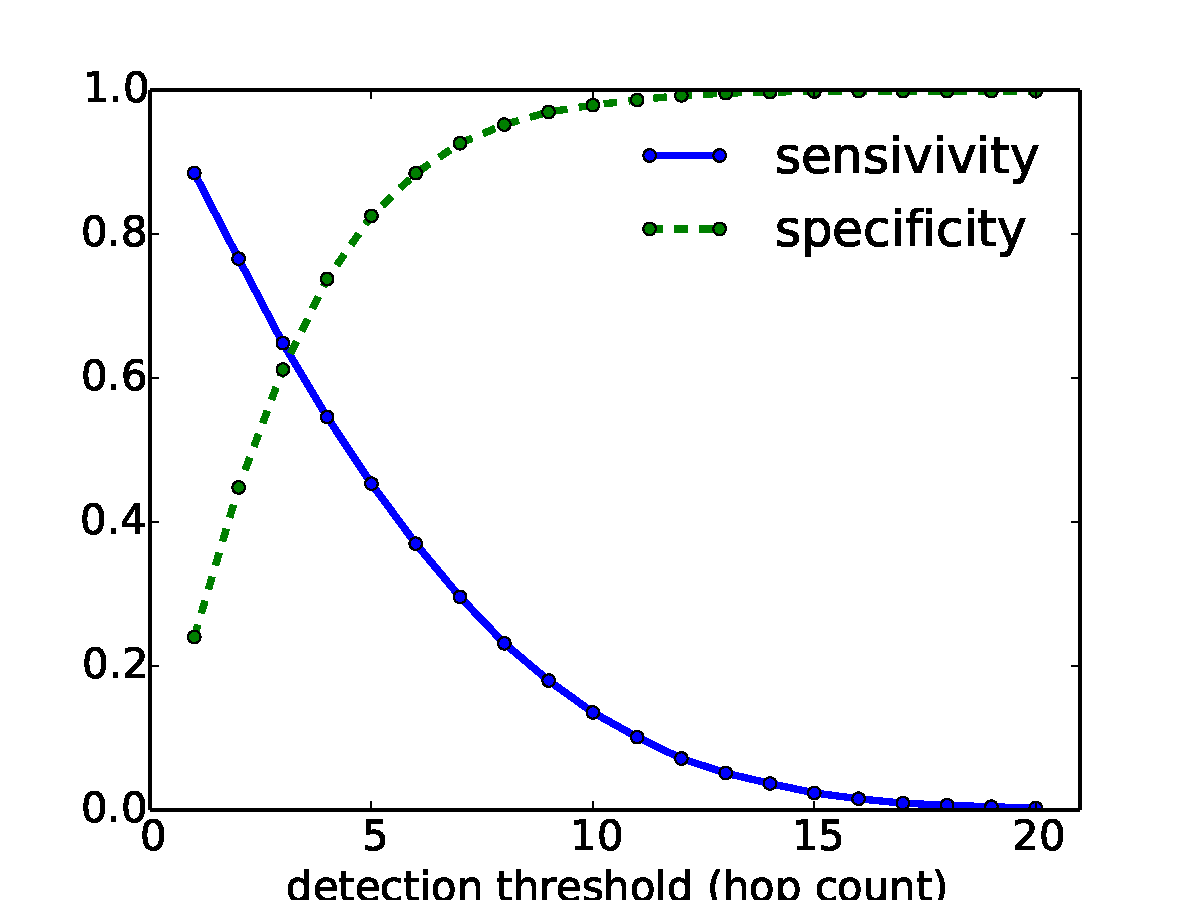
\includegraphics[width=.49\linewidth]{Graph/spoof/sens-spec-accuracy-caida-jun2015-source-to-monitor-ttls-2000files-sample10000.pdf}
	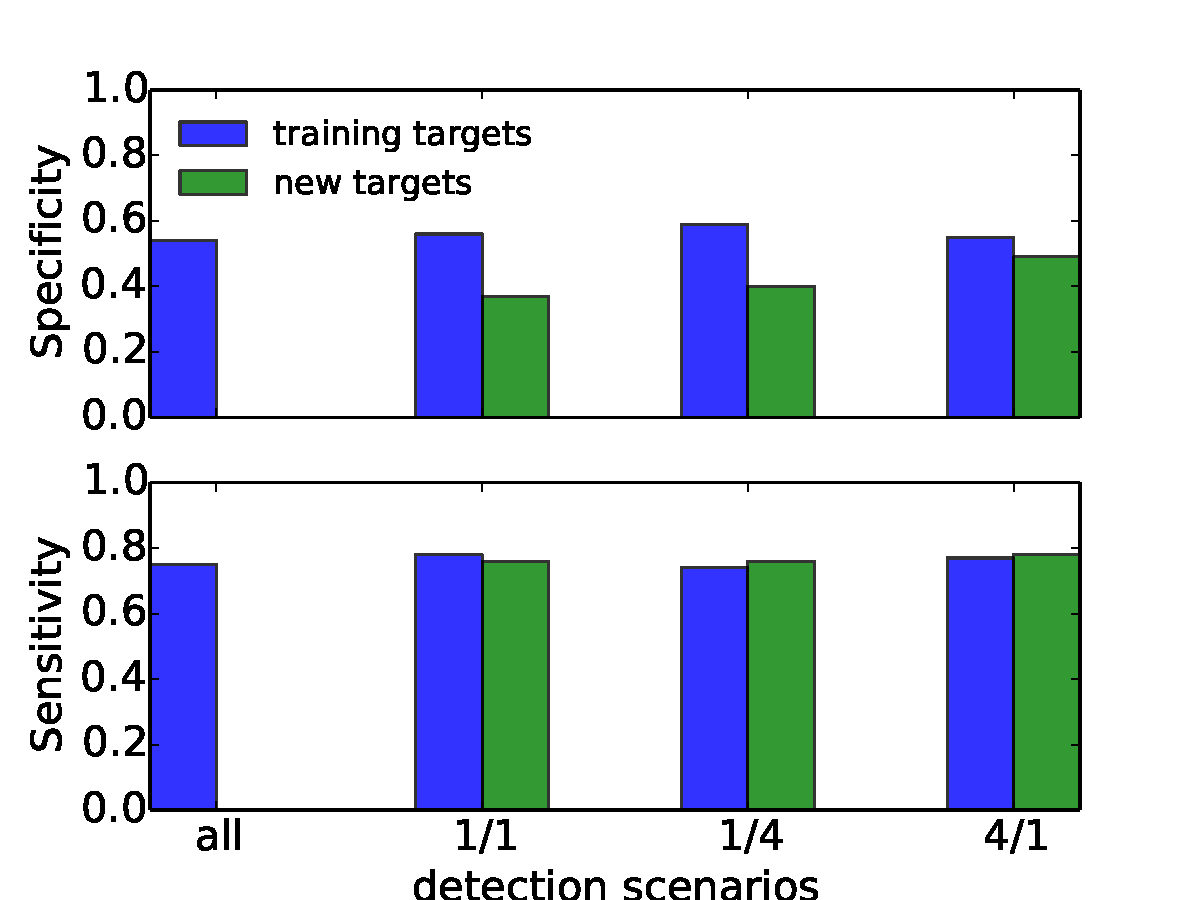
\includegraphics[width=.49\linewidth]{Graph/spoof/accuracy-bars.pdf}
	\caption{Detector accuracy under various scenarios. (left) We run detection on the  same targets used in training and vary the detection threshold; increasing the threshold reduces sensitivity and improves specificity; (right) We perform detection using both training targets and new targets not used in the training process; we set the detection threshold to two hops (the average estimation error of the model); as we vary the ratio between training and detection targets, the sensitivity for the new targets is comparable to that of the training targets, while the specificity is lower; ``all'' indicates that we perform training and detection on all targets, therefore there are no new targets.}
	\label{fig:sens}
	\vspace{0.5cm}
\end{figure*}

{\bf Summary.} Learning maps can trade-off high accuracy in detecting spoofed traffic with a high rate of false positives. This indicates that learning maps could be an important part of a bigger framework for spoofing detection, which could process the false alarms faster or dynamically adjust the detection threshold to control their rate.

\subsubsection{Model transfer} 
\label{spoof:transfer}

To understand whether our learned model is general and can be transferred to new hosts, we split the data set into two disjoint sets, such that the targets in each set are disjoint. We train a model using only the targets in the first set and then run detection on both sets. Our goal is to understand how the detector performance for a target changes when we use a model learned for other targets. We consider three different splits: the number of targets in each set is the same (``1/1'' split), the number of training targets is four times larger (``4/1'' split) and, the training targets are four times fewer (``1/4'' split). We set the detection threshold at two hops and compute the average sensitivity and specificity for spoofing detection on each set across all splits. 

Figure~\ref{fig:sens}(right) presents the results. The sensitivity of targets not part of the training process is comparable to that of those targets used in training, showing that our models are transferable to new targets with little loss in accuracy. This reduces the cost of global deployment as new targets do not need to gather training data and build their own models. An interesting observation from Figure~\ref{fig:sens} is that the specificity of new targets is lower than for training targets: raising false alerts is more likely on hosts not part of the training.

{\bf Summary.} Maps learned at a single location are transferable to other servers in the Internet with little loss in accuracy. This is because maps are learned based on structural network properties that are the same from every vantage point and do not depend on specific locations. 


\subsubsection{Performance}

Training a representative embedding does not require significant resources. Learning a model with hop counts from 100,000 IPs to 96 servers takes about one hour on a server with four 3.5GHz quad-core Intel Xeon processors and 128GB of RAM (Table~\ref{tab:performance}). Each model takes less than 5MB of memory and thus is easily transferable over the network. Detection is fast as well. Using the same machine used for training, and given an IP packet, we are able to decide whether the packet is spoofed or not in under a millisecond. While running the detector at line speed on a network gateway instead of a powerful GPU machine may reduce these numbers, recent deep learning platforms, such as Net2Vec~\citep{net2vec}, that are able to capture and process packets at 60Gbps can make deployment easier and faster.

\begin{table}[]
	\centering
	\begin{tabular}{l|c|c|c}
		{\bf Number of source IPs}   & 1,000 & 10,000 & 100,000 \\
		\hline
		{\bf Time to train (min)} &  1 & 6 & 58\\
		\hline
		{\bf Size of model (MB)} & 4.5 & 4.5 & 4.5\\
	\end{tabular}
	\caption{Performance of training for data sets containing hop count information from 96 servers to 1,000, 10,000, and 100,000 IPs. Each data set is sparse, with only about 15\% of all entries available.}
	\label{tab:performance}
	% \vspace{-0.5cm}
\end{table}

\subsection{Discussion: Limitations and opportunities}
\label{spoof:discussion}

%We discuss several aspects related to the accuracy and deployment of our learning-based spoofing detection.

{\bf Accuracy trade-off.} Our detector trades off accuracy for generality. Low specificity may be unacceptable for many operators, who would still need to sift through alerts to identify legitimate packets incorrectly identified as spoofed. In practice, we envision that our approach works in conjunction with network-based maps and host maps built from passive measurements to offer a comprehensive and cost-efficient spoofing detection solution.

{\bf Non-metric Internet.}
Paths between Internet hosts are dictated by routing policies and AS peering agreements, and are not always shortest in terms of hop counts. Estimating the hop count between two hosts as the Euclidean distance between their embeddings does not capture the intricacies of Internet routing and may introduce errors. We are working on reducing these errors in two ways. First, we plan to introduce AS membership as an additional data set in the deep learning framework. Knowing to which AS a host belongs to can help constrain its possible positions in the embedding space. Second, we plan to add IP addresses and hop counts to routers on the path between a source and a destination. While a perfect metric embedding of Internet hop counts is impossible~\citep{peerwise}, we can reduce the learning error and better predict anomalies.

Furthermore, we are exploring non-metric embeddings. It is possible to learn structural embeddings of the Internet that estimate other network properties helpful in spoofing detection. For example, graph embeddings preserve local and remote network structure features such as first- and second-order neighbors~\citep{net-emb}. We are investigating how to use such mechanisms to devise spoofing detectors that avoid the shortcomings of hop based spoofing detection.

{\bf Dynamic Internet.}
The dynamic nature of the Internet with frequent misconfigurations, outages, or policy changes means that hop counts or IP addresses may also change~\citep{cunha, reasons}. If this happens, we may need to retrain the embedding model to reflect the updated values. A practical deployment would passively listen to incoming legitimate traffic, or selectively probe IPs from learned maps, and update existing maps to reflect new hop count values. We are currently working on how to re-train our model to learn a more accurate hop count estimation in the presence of new hop count data.

{\bf Asymmetric Internet.}
Internet routing may not always be symmetric~\citep{asym}. Due to ISP routing practices, the direct and reverse route between two nodes may be different, resulting in potentially different hop count measurements between the same pair of nodes. Because we compute hop count information from TTL values decremented exclusively by routers on the {\em direct} path between source IPs and targets, our detection is not impaired by the routing asymmetry.

{\bf Bootstrapping.} Learning a representative structural model of the Internet requires hop count measurements from many vantage points. Not all enterprises have access to many geographically distributed monitors to collect hop count data for the initial model training. There are two possibilities to generate learned maps in such scenarios. First, one could use third-party measurement data, such as that provided by CAIDA~\citep{ark}, to train a descriptive model and generate learned maps. 
%Because we use deep learning to train models, one can easily incorporate new data sources (\eg{}, AS membership information) by adding new layers or neurons. 
Second, an enterprise could deploy a model already trained in another location. As we showed in Section~\ref{spoof:transfer}, our models are transferable with little loss in accuracy. 


{\bf Attack types.}
We assumed a spoofing attack carried by a random attacker without any knowledge of the network topology. In reality, some attackers may be able to obtain information about the network that could help subvert the defense. For example, if an attacker controls multiple bots, it can send the attack from the bots that have a more popular hop count value to the target. This maximizes the likelihood of passing by our filter as there are more IP addresses with which to spoof the source.
%
Furthermore, if the attacker learns the hop count between the spoofed IP and the target, it can also spoof the TTL field of the attack packets, inserting a value that corresponds to the learned hop count. In this case, no hop count filtering can detect the attack. To learn the hop count between two arbitrary hosts, one can use DIP~\citep{dip}, the same framework we employ, or the algorithm described by Barford~\etal{}~\citep{barford-infocom}. However, both mechanisms require coordination and control of multiple geographically distributed servers, available only to more complex attackers.










\chapter{Extracing Latent Information from Abandoned Speech Interpretations}
\label{ch:nbest}

In a modern spoken language understanding (SLU) system, the natural language understanding (NLU) module takes interpretations of a speech from the automatic speech recognition (ASR) module as the input. The NLU module usually uses the first best interpretation of a given speech in downstream tasks such as domain and intent classification. However, the ASR module might misrecognize some speeches and the first best interpretation could be erroneous and noisy. Solely relying on the first best interpretation could make the performance of downstream tasks non-optimal especially when the ASR model does not perform well. To address this issue, we introduce a series of simple yet efficient models for improving the understanding of semantics of the input speeches by collectively exploiting the $n$-best speech interpretations from the ASR module. 

\section{Introduction}
\label{alexa:intro}
Currently, voice-controlled smart devices are widely used in multiple areas to fulfill various tasks, e.g. playing music, acquiring weather information and booking tickets. 
The SLU system employs several modules to enable the understanding of the semantics of the input speeches. 
When there is an incoming speech, the ASR module picks it up and attempts to transcribe the speech.
An ASR model could generate multiple interpretations for most speeches, which can be ranked by their associated confidence scores.
% ({\color{red} add figure here})
Among the $n$-best hypotheses, the top-1 hypothesis is usually transformed to the NLU module for downstream tasks such as domain classification, intent classification and named entity recognition (slot tagging). Multi-domain NLU modules are usually designed hierarchically \citep{tur2011spoken}. For one incoming utterance, NLU modules will firstly classify the utterance as one of many possible domains and the further analysis on intent classification and slot tagging will be domain-specific.


% For the coming utterances, they will firstly convert the text with \textit{byte pair encoding} (BPE) \citep{gage1994new} for word segmentation and perform the domain classification by Multilayer per ceptrons (MLP)  to classify the utterance as one of many possible domains. Then, the further analysis on intent classification and slot tagging will be domain-specific. 
In spite of impressive development on the current SLU pipeline, the interpretation of speech could still contain errors.
Sometimes the top-1 recognition hypothesis of ASR module is ungrammatical or implausible and far from the ground-truth transcription \citep{peng2013search, jyothi2012large}. 
Among those cases, we find one interpretation exact matching with or more similar to transcription can be included in the remaining hypotheses ($2^{nd}- n^{th}$). 

To illustrate the value of the $2^{nd}- n^{th}$ hypotheses, we count the frequency of exact matching and more similar (smaller edit distance compared to the $1^{st}$ hypothesis) to  transcription for different positions of the $n$-best hypotheses list.
% Moreover, we count the times that one interpretation within the $2^{nd}$ to $n^{th}$ best is more similar to transcription than the $1^{st}$ best by the measurement of edit distance between hypotheses and transcription. 
Table \ref{tbl:nbest} exhibits the results. For the explored dataset, we only collect the top 5 interpretations for each utterance ($n = 5$). Notably, when the correct recognition exists among the 5 best hypotheses, 50\% of the time (sum of the first row's percentages) it occurs among the $2^{nd}-5^{th}$ positions. Moreover, as shown by the second row in Table \ref{tbl:nbest}, compared to the top recognition hypothesis, the other hypotheses can sometimes be more similar to the transcription. 



\begin{table}[h]
	\vspace{-1.5ex}
	\captionof{table}{Spoken recognition quality distribution of the $n$ best hypotheses.}
	\label{tbl:nbest}
	\centering
	\begin{tabular}{|c|c c c c|} 
		\hline
		$n$ Best Rank Position & $2^{nd}$ & $3^{rd}$ & $4^{th}$ & $5^{th}$ \\
		\hline
		Match&19\%&14\%&10\%&7\%\\
		Prob (better than $1^{st}$ best) & 22\%&17\%&16\%&15\%\\
		\hline
	\end{tabular}
	\vspace{-2ex}
\end{table}

Over the past few years, we have observed the success of reranking the $n$-best hypotheses 
\citep{peng2013search, charniak2005coarse, morbini2012reranking,  dikici2012classification, Sak2011DiscriminativeRO, sak2010fly,discriminative, collins2005discriminative, chan2004improving}
before feeding the best interpretation to the NLU module. These approaches propose the reranking framework by involving morphological, lexical or syntactic features \citep{discriminative, collins2005discriminative, chan2004improving}, speech recognition features like confidence score \citep{peng2013search, morbini2012reranking}, and other features like number of tokens, rank position \citep{peng2013search}.  They are effective to select the best from the hypotheses list and reduce the word error rate (WER) \citep{oba2007approach} of speech recognition. 
% There have been some early models working on the ASR $n$-best hypotheses \citep{peng2013search, charniak2005coarse, morbini2012reranking,  dikici2012classification, Sak2011DiscriminativeRO, sak2010fly}. With a pre-trained model classifying hypothesis to different domains or intents, \citep{morbini2012reranking} has tried to evaluate separately for each of the $n$ hypotheses, to merge and rerank the results. Alternatively, in \citep{peng2013search}, a binary classification model is used to formulate the reranking problem of $n$ best hypotheses according to the hypotheses' features like rank position, number of tokens, etc. Similarly, others \citep{discriminative, collins2005discriminative, chan2004improving} explore the morphological, lexical or syntactic features for the reranking model. Those methods are effective to choose the best from the hypotheses list. 

Those reranking models could benefit the first two cases in Table \ref{tbl:expMotiv} when there is an utterance matching with transcription. However, in other cases like the third row, it is hard to integrate the fragmented information  in multiple hypotheses. 

This paper proposes various methods integrating $n$-best hypotheses to tackle the problem. To the best of our knowledge, this is the first study that attempts to collectively exploit the $n$-best speech interpretations in the SLU system.  This paper serves as the basis of our $n$-best-hypotheses-based SLU system, focusing on the methods of integration for the hypotheses. 
Since further improvements of the integration framework require considerable setup and descriptions, where jointly optimized tasks (e.g. transcription reconstruction) trained with multiple ways (multitask \citep{caruana1997multitask}, multistage learning \citep{gong2013multi}) and more features (confidence score, rank position, etc.) are involved, we leave those to a subsequent article.

% we will leave the  discussion about using more tasks (e.g. transcription reconstruction) with multiple ways (multitask \citep{caruana1997multitask}, multistage learning \citep{gong2013multi}) and involving more features (confidence score, rank position, etc.) in integration framework for further improvements in a subsequent article.  

% The.........

% In this paper, we will focus on the discussion ...., which serves our basic in the whole system..., This work is the first part of ... system. The furhter discussion about ... will be elaberated on our next paper.
% introduction end, discussion related work, mikolov 

% To the best of our knowledge, ...
% Seperate process of 
% not influence the embedding of words: "Bose" "Bowls" 
% Mikolov's paper
% pooling with sliding window n*1 stride 1, 

\begin{table}[t!]
	\captionof{table}{Motivating example: comparison of ASR $n$-Best hypotheses with the corresponding transcription. }
	\label{tbl:expMotiv}
	\centering
		\begin{tabular}{|c|c|c|c|}
			\hline
			
			Transcription& $1^{st}$ best &$2^{nd}$ best&$3^{rd}$ best \\
			% \multicolumn{2}{|c|}{Transcription} & \multicolumn{2}{|c|}{Transcription} & \multicolumn{2}{|c|}{Transcription} & \multicolumn{2}{|c|}{Transcription} \\
			\hline
			\textbf{play muse}&play news&\textbf{play muse}&play mus\\
			\textbf{track on bose}&check on bowls& check on bose &\textbf{track on bose}\\
			\textbf{harry porter} & how \textbf{porter}& how patter&\textbf{harry} power\\
			\hline
			
		\end{tabular}
		

\end{table}


This paper is organized as follows. Section \ref{speech:pretrain} introduces the Baseline, Oracle and Direct models. Section \ref{speech:models} describes proposed ways to integrate $n$-best hypotheses during training. The experimental setup and results are described in Section \ref{speech:exp}. Section \ref{speech:conclusion} contains conclusions and future work.


\section{Baseline, Oracle and Direct Models}
\label{speech:pretrain}

\subsection{Baseline and Oracle}

The preliminary architecture is shown in Fig. \ref{fig:traditional}. For a given transcribed utterance, it is firstly encoded with Byte Pair Encoding (BPE) \citep{sennrich2015neural}, a compression algorithm splitting words to fundamental subword units (\textit{pairs of bytes} or \textit{BP}s) and reducing the embedded vocabulary size. Then we use a BiLSTM \citep{schuster1997bidirectional} encoder and the output state of the BiLSTM is regarded as a vector representation for this utterance. Finally, a fully connected Feed-forward Neural Network (FNN) followed by a softmax layer, labeled as a multilayer perceptron (MLP) module, is used to perform the domain/intent classification task based on the vector.


% For the coming utterances, they will firstly convert the text with \textit{byte pair encoding} (BPE) \citep{gage1994new} for word segmentation and perform the domain classification by Multilayer perceptrons (MLP)  to classify the utterance as one of many possible domains. Then, the further analysis on intent classification and slot tagging will be domain-specific. 


\begin{figure}[!htp]
	\centering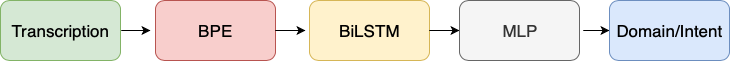
\includegraphics[width=0.8\textwidth]{Graph/speech/Baseline.png}
	\caption{Baseline pipeline for domain or intent classification.}
	\label{fig:traditional}
\end{figure}


% In this work, we set the model trained with transcription as our baseline model and use model performance on ASR 1best as the baseline results, given that this is how the state of the art models are trained and evaluated. We also use the results from the same model but tested using transcription as an upper bound results. The reason why we call this result upper bound is because that we assume that 

For convenience, we simplify the whole process in Fig.\ref{fig:traditional} as a mapping $BM$ (Baseline Mapping) from the input utterance $S$ to an estimated tag's probability $p(\Tilde{t})$, where $p(\Tilde{t}) \leftarrow BM(S)$.
% \begin{equation}
%  \vspace{-1ex}
% \small{
%  p(\Tilde{t}) \leftarrow BM(S)
%  \label{simplify}
%  }
%  \vspace{-1ex}
%  \end{equation}
The $Baseline$ is trained on transcription and evaluated on ASR $1^{st}$ best hypothesis ($S=\text{ASR}\ 1^{st}\  \text{best})$. The $Oracle$ is trained on transcription and evaluated on transcription ($S = \text{Transcription}$). We name it Oracle simply because we assume that hypotheses are noisy versions of transcription. 
%All the approaches (Baseline, Oracle and methods in Section \ref{subspeech:combination}) exploiting the BM mapping trained on transcription are named as \textit{direct models}.
\subsection{Direct Models}
\label{subspeech:combination}

Besides the Baseline and Oracle, where only ASR 1-best\footnote{We use ASR \textit{$n$-best hypotheses} or $n$-bests to denote the top $n$ interpretations of a speech, and the \textit{1,5-best} standing for the top 1 or 5 hypotheses.} 
hypothesis is considered, we also perform experiments to utilize ASR $n$-best hypotheses during evaluation. The models evaluating with $n$-bests and a BM (pre-trained on transcription) are called \textit{Direct Models} (in Fig. \ref{fig:eval}):

\begin{figure}[!htp]
	\vspace{2em}
	\centering
	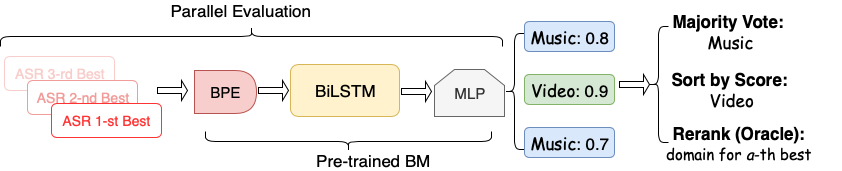
\includegraphics[width=0.95\textwidth]{Graph/speech/Evaluate.png}
	\caption{Direct models evaluation pipeline.}
	\label{fig:eval}
	
\end{figure}

\begin{itemize}
	\item \textit{Majority Vote.} We apply the BM model on each hypothesis independently and combine the predictions by picking the majority predicted label, i.e. Music.
	\vspace{-1ex}
	\item \textit{Sort by Score.} After parallel evaluation on all hypotheses, sort the prediction by the corresponding confidence score and choose the one with the highest score, i.e. Video.
	\vspace{-1ex}
	\item \textit{Rerank (Oracle).} 
	Since the current rerank models (e.g., \citep{peng2013search, charniak2005coarse, morbini2012reranking}) attempt to select the hypothesis most similar to transcription, we propose the Rerank (Oracle), which picks the hypothesis with the smallest edit distance to transcription (assume it is the $a$-th best) during evaluation and uses its corresponding prediction. 
	
\end{itemize}


% For these results, we apply the BM model on each hypothesis independently and use different aggregation approach to combine prediction from all hypotheses. The Majority Vote approach picks the majority predicted label from all hypotheses, while the Sort by Score approach ranks all the predicted labels by the predictive probability. Another approach assumes that we are able to pick the best hypothesis, which has the minimum edit distance from transcript, and uses its corresponding prediction. 
\section{Integration of N-BEST Hypotheses}
\label{speech:models}
All the above mentioned models apply the BM trained on one interpretation (transcription). Their abilities to take advantage of multiple interpretations are actually not trained. As a further step, we propose multiple ways to integrate the $n$-best hypotheses during training. The explored methods can be divided into two groups as shown in Fig. \ref{fig:integration}. Let $H_1, H_2,..., H_n $ denote all the hypotheses from ASR and $bp_{H_k, i} \in BPs$ denotes the $i$-th pair of bytes (BP) in the $k^{th}$ best hypothesis. The model parameters associated with the two possible ways both contain: embedding $e_{bp}$ for pairs of bytes, BiLSTM parameters $\theta$ and MLP parameters $W, b$.

\begin{figure}[t!]
	\vspace{2em}
	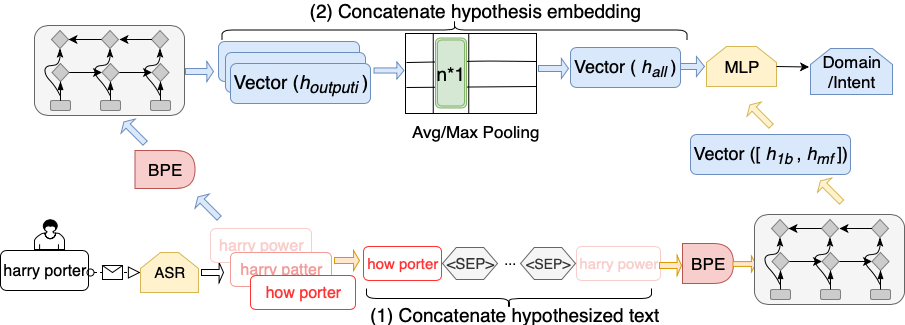
\includegraphics[width=0.9\textwidth]{Graph/speech/Compress.png}
	\vspace{1em}
	\caption{Integration of $n$-best hypotheses with two possible ways: 1) concatenate hypothesized text  and 2) concatenate hypothesis embedding.}
	\label{fig:integration}
\end{figure}

\subsection{Hypothesized Text Concatenation}
The basic integration method (\textit{Combined Sentence}) concatenates the $n$-best hypothesized text. We separate hypotheses with a special delimiter ($<$SEP$>$). We assume BPE totally produces $m$ BPs (delimiters are not split during encoding). Suppose the $n^{th}$ hypothesis has $j$ pairs. The entire model can be formulated as:
\begin{equation}
\small{
	(h_1, ... , h_m)\leftarrow BiLSTM_{\theta}(bp_{H_1, 1},...,bp_{<sep>},...,bp_{H_n, j})
}
\label{bilstm}
\end{equation}
\begin{equation}
\small{
	p(\Tilde{t}) = \sigma(W[h_{1b}, h_{mf}] +b)
}
\label{mlp}
\end{equation}
In Eqn. \ref{bilstm}, the connected hypotheses and separators are encoded via BiLSTM to a sequence of hidden state vectors. Each hidden state vector, e.g. $h_1$, is the concatenation of forward $h_{1f}$ and backward $h_{1b}$ states. The concatenation of the last state of the forward and backward LSTM forms the output vector of BiLSTM (concatenation denoted as $[,]$). Then, in Eqn. \ref{mlp}, the MLP module defines the probability of a specific tag (domain or intent)  $\Tilde{t}$ as the normalized activation ($\sigma$) output  after linear transformation of the output vector.

%  the MLP module firstly concatenates the last state of the forward and backward LSTM for the $m$ pairs of bytes (concatenation operation denoted as $[,]$) as final output vector. Then, it defines the probability of a specific tag (domain or intent)  $\Tilde{t}$ as the normalized activation ($\sigma$) output  after linear transformation of the output vector.


\subsection{Hypothesis Embedding Concatenation}
The concatenation of hypothesized text leverages the $n$-best list by transferring information among hypotheses in an embedding framework, BiLSTM. However, since all the layers have access to both the preceding and subsequent information, the embedding among $n$-bests will influence each other, which confuses the embedding and makes the whole framework sensitive to the noise in hypotheses.

As the second group of integration approaches, we develop models, \textit{PoolingAvg/Max}, on the concatenation of hypothesis embedding, which isolate the embedding process among hypotheses and summarize the features by a pooling layer. For each hypothesis (e.g., $i^{th}$ best in Eqn. \ref{bilstm_1} with $j$ pairs of bytes), we could get a sequence of hidden states from BiLSTM and obtain its final output state by concatenating the first and last hidden state ($h_{output_i}$ in Eqn. \ref{output}).
% The final output state for an utterance can be generated through concatenating its first and last hidden state. 
Then, we stack  all the output states vertically as shown in Eqn. \ref{outputs}. Note that in the real data, we will not always have a fixed size of hypotheses list. For a list with $r$ ($<n$) interpretations, we get the embedding for each of them and pad with the embedding of the first best hypothesis until a fixed size $n$. When $r\geq n$, we only stack the top $n$ embeddings. We employ $h_{output_1}$ for padding to enhance the influence of the top 1 hypothesis, which is more reliable. Finally, one unified representation could be achieved via    \textit{Pooling} (Max/Avg pooling with $n$ by 1 sliding window and stride 1)  on the concatenation and one score could be produced per possible tag for the given task. 
\begin{equation}
\small{
	(h_{H_i, 1}, ... , h_{H_i, j})\leftarrow BiLSTM_{\theta}(bp_{H_i, 1},...,bp_{H_i, j})
}
\label{bilstm_1}
\end{equation}
\begin{equation}
\small{
	h_{output_i} = [h_{H_i, 1b},\ h_{H_i, jf}]
	\label{output}
}
\end{equation}
\begin{equation}
\small{
	h_{outputs} = \begin{Bmatrix}
	
	\begin{Bmatrix}
	h_{output_1}\\...\\ h_{output_r}
	\end{Bmatrix} & r-bests
	\\
	\begin{Bmatrix}
	h_{output_1}\\ ...
	\end{Bmatrix} & Padding\ with\ h_{output_1}
	\end{Bmatrix}
}
\label{outputs}
\end{equation}
\begin{equation}
\small{
	h_{all} = Pooling(h_{outputs})
}
\label{pooling}
\end{equation}
\begin{equation}
\small{
	p(\Tilde{t}) = \sigma(Wh_{all} +b)
}
\label{mlp_1}
\end{equation}
\section{Experiment}
\label{speech:exp}
\subsection{Dataset}
% We conduct our experiments on an SLU system serving the Alexa-enabled device. There are $\sim$ 8.7M utterances annotated and derived from requests across 23 domains. The $n$-bests list collected from ASR for each utterance contains no more than 5 hypotheses ($n=5$). For domain classification, the models work on the entire data. While for the intent classification task, we choose three popular domains for domain-specific intent classification. 
We conduct our experiments on $\sim$ 8.7M annotated anonymised user utterances. They are annotated and derived from requests across 23 domains. 
% To simulate the usage with  not so high-quality ASR recognition results,
% some further cleaning techniques after ASR recognizing  are not considered. The discussion for integrating high-quality ASR recognition results, which are closer to the Oracle model, is left as the future work.
% the wake words of hypotheses are not removed.
\subsection{Performance on Entire Test Set}

% Table \ref{tbl:entire dataset} shows the Micro and Macro F1 score and relative error reduction (RErr)\footnote{The RErr for a model $m$ is calculated by comparing the relative difference between $100\% - MicroF1_{m}$ and $100\% - MicroF1_{\text{Baseline}}$.  } of Baseline, Oracle and our proposed models on the entire test set ($\sim$ 300K utterances) for multi-class domain classification. 
Table \ref{tbl:entire dataset} shows the relative error reduction (RErr)\footnote{The RErr for a model $m$ is calculated by comparing the relative difference between $100\% - MicroF1_{m}$ and $100\% - MicroF1_{\text{Baseline}}$.  } of Baseline, Oracle and our proposed models on the entire test set ($\sim$ 300K utterances) for multi-class domain classification. 
% For the direct models, we train one baseline model on transcription and corresponding domains. Then, we evaluate based on transcription (\textit{Upper Bound}), ASR $1^{st}$ Best hypothesis (\textit{Baseline}), the hypothesis most similar to transcription (\textit{Rerank (Oracle)})  and predict $n$ times for all of the ASR hypotheses to combine the results by \textit{Majority voting} or \textit{Sort by Score}. 
We can see among all the direct methods, predicting based on the hypothesis most similar to the transcription (Rerank (Oracle)) is the best.


% This also reveals the limit of the methods using the pre-trained model. 

%willing to pick one from the hypotheses list by choose the best one 

% For the pre-trained models, we train a baseline model $M$, which includes the embedding of hypothesis, BiLSTM and MLP, based on the transcriptions and corresponding domains in training set. 
% \begin{table}[h]
% \centering
% \captionof{table}{Micro and Macro F1 score for multi-class domain classification.}
% \vspace{-1ex}
% \label{tbl:entire dataset}
% \scalebox{0.8}{
%  \begin{tabular}{ c|c |c c c} 
%  \hline
% Category & Model & Micro F1 & RErr(\%) &Macro F1 \\
% \hline
% \multicolumn{2}{c|}{Baseline}			& \textbf{90.83}&	\textbf{0.00}	& \textbf{87.15} \\
% \hline
% \multirow{3}*{Integration}&PoolingAvg			& \textbf{92.14}	& \textbf{14.29} &	\textbf{89.1} \\
% &PoolingMax		& 92.04	& 13.20 &	88.99\\
% &Combined Sentence	& 91.9	& 11.67 &	88.7\\
% % &CNN					& 89.73&	-12.00	& 83.5\\
% \hline
% \multirow{3}*{Direct}&Sort by Score		& 91	&1.85	& 87.33\\
% &Majority Vote		& 90.98&	1.64	& 87.33\\
% &Rerank (Oracle)		& \textbf{91.17}&	\textbf{3.71}	& \textbf{87.8} \\
% \hline
% \multicolumn{2}{c|}{Oracle}			& 93.31	&27.04	& 90.84\\
% \hline
% \end{tabular}}
% \vspace{-2ex}
% \end{table}
\begin{table}[h]
	\centering
	\captionof{table}{Micro and Macro F1 score for multi-class domain classification.}
	\vspace{-1ex}
	\label{tbl:entire dataset}
	\scalebox{0.8}{
		\begin{tabular}{ c|c|c} 
			\hline
			Category & Model & RErr(\%)  \\
			\hline
			\multicolumn{2}{c|}{Baseline}& 	\textbf{0.00} \\
			\hline
			\multirow{3}*{Integration}&PoolingAvg	& \textbf{14.29} \\
			&PoolingMax		& 13.20 \\
			&Combined Sentence		& 11.67 \\
			% &CNN					& 89.73&	-12.00	& 83.5\\
			\hline
			\multirow{3}*{Direct}&Sort by Score		&1.85\\
			&Majority Vote	&	1.64\\
			&Rerank (Oracle)	&	\textbf{3.71}   \\
			\hline
			\multicolumn{2}{c|}{Oracle}		&27.04\\
			\hline
	\end{tabular}}

\end{table}

As for the other models attempting to integrate the $n$-bests during training, PoolingAvg gets the highest relative improvement, 14.29\%. It as well turns out that all the integration methods outperform direct models drastically. This shows that having access to $n$-best hypotheses during training is crucial for the quality of the predicted semantics. 
% \subsection{ASR First Best Agree with Transcription or not}
\subsection{Performance Comparison among Various Subsets}

\begin{table}[ht]
	\centering
	\captionof{table}{Performance comparison for the subset ($\sim$ 19\%) where ASR first best disagrees with transcription.}
	\vspace{-1ex}
	\label{tbl:disagree}
	\scalebox{0.8}{
		\begin{tabular}{ c|c|c} 
			\hline
			Category & Model &  RErr(\%)  \\
			\hline
			\multicolumn{2}{c|}{Baseline}&	\textbf{0.00}\\
			\hline
			\multirow{3}*{Integration}&PoolingAvg&	24.67\\
			&PoolingMax	&	26.23\\
			&Combined Sentence&	19.23\\
			% &CNN												&79.07&	12.10&	75.16\\
			\hline
			\multirow{3}*{Direct}&Sort by Score	&	9.95\\
			&Majority Vote&	7.59\\
			&Rerank (Oracle)&	7.25\\
			\hline
			\multicolumn{2}{c|}{Oracle}	&53.02\\
			
			
			
			\hline
	\end{tabular}}
\end{table}


\begin{table}[h]
	\centering
	\captionof{table}{Performance comparison for the subset ($\sim$ 81\%) where ASR first best agrees with transcription.}
	\vspace{-1ex}
	\label{tbl:agree}
	\scalebox{0.8}{
		\begin{tabular}{ c|c |c} 
			\hline
			Category & Model & RErr(\%) \\
			\hline
			\multicolumn{2}{c|}{Baseline}	&	\textbf{0.00}\\
			\hline
			\multirow{3}*{Integration}&PoolingAvg &	3.56\\
			&PoolingMax										&-0.38\\
			&Combined Sentence									&	4.50\\
			% &CNN												&92.35	&-39.0& 85.22\\
			\hline
			\multirow{3}*{Direct}&Sort by Score	&	-8.269\\
			&Majority Vote		&	-3.19\\
			&Rerank (Oracle)	&	0.00\\
			
			\hline
			\multicolumn{2}{c|}{Oracle}	&	0.00\\
			\hline
	\end{tabular}}

\end{table}

To further detect the reason for improvements, we split the test set into two parts based on whether ASR first best agrees with transcription (ignore difference with wake words of hypotheses) and evaluate separately. Comparing Table \ref{tbl:disagree} and Table \ref{tbl:agree}, obviously the benefits of using multiple hypotheses are mainly gained when  ASR $1^{st}$ best disagrees with the transcription. When ASR $1^{st}$ best agrees with transcription, the proposed integration models can also keep the performance. Under that condition, we can still improve a little (3.56\%) because, by introducing multiple ASR hypotheses, we could have more information and when the transcription/ASR $1^{st}$ best does not appear in the training set's transcriptions, its $n$-bests list may have similar hypotheses included in the training set's $n$-bests. Then, our integration model trained on $n$-best hypotheses as well has clue to predict. 
% , which makes the integration models can tackle the ambiguous condition (the same transcription can be annotated to different domains \citep{xu2014contextual} but at this time their $n$-bests lists can be distinguishable) and still improve a little when ASR first best agrees with transcription.
The series of comparisons reveal that our approaches integrating the hypotheses are robust to the ASR errors and whenever the ASR model makes mistakes, we can outperform more significantly. 
% Our conjecture is that the more benefits using all n-best hypotheses when the ASR 


\subsection{Improvements on Different Domains and Different Numbers of Hypotheses}
Among all the 23 domains, we choose 8 popular domains for further comparisons between the Baseline and the best model of Table \ref{tbl:entire dataset}, PoolingAvg. Fig. \ref{fig:important} exhibits the results.  PoolingAvg consistently improves the accuracy for all 8 domains.

In the previous experiments, the number of utilized hypotheses for each utterance during evaluation is five, which means we use the top 5 interpretations when the size of ASR recognition list is not smaller than 5 and use all the interpretations otherwise. Changing the number of hypotheses while evaluation, Fig. \ref{fig:amount} shows a monotonic increase with the access to more hypotheses for the PoolingAvg and PoolingMax (Sort by Score is shown because it is the best achievable direct model while the Rerank (Oracle) is not realistic). The growth becomes gentle after four hypotheses are leveraged. 
\begin{figure}[h]
	\centering
	\scalebox{1}{
		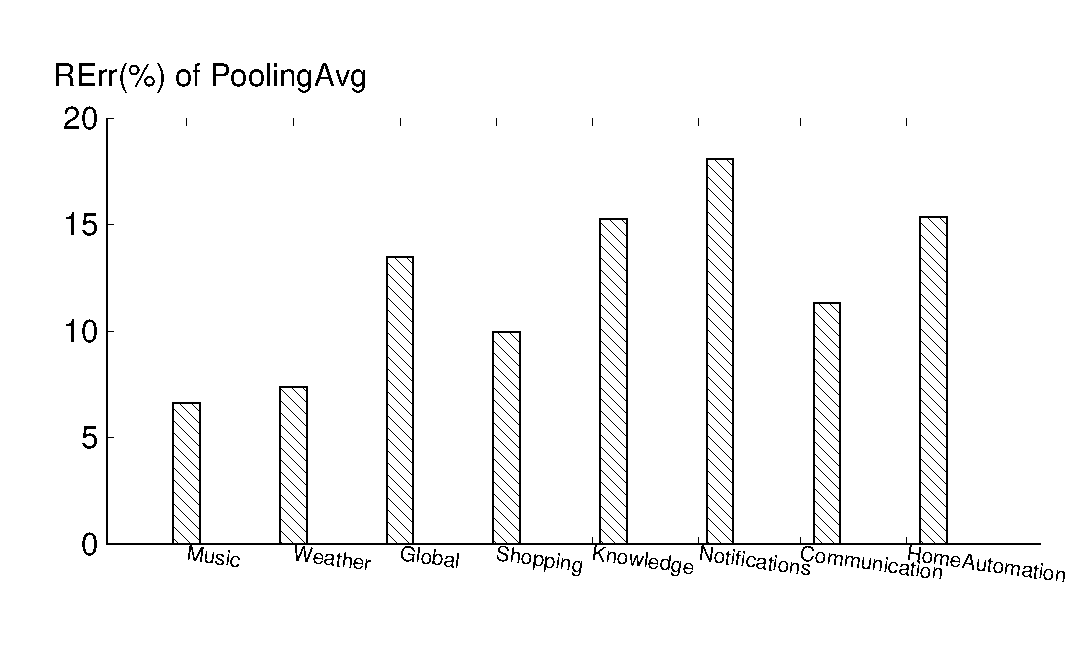
\includegraphics[width=0.7\textwidth]{Graph/speech/barRelative.eps}
	}

	\caption{Improvements on important domains.}
	\label{fig:important}

	
\end{figure}
% \subsection{Different Amount of Hypotheses}

\begin{figure}[h]
	\centering

	\scalebox{0.8}{
		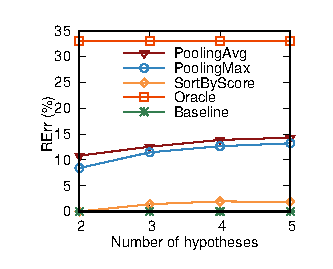
\includegraphics[width=0.7\textwidth]{Graph/speech/ASRAmountRelative.eps}
	}

	\caption{The influence of different amount of hypotheses.}

	\label{fig:amount}
	
\end{figure}

\subsection{Intent Classification}
\begin{table}[!htp]
	\captionof{table}{Intent classification for three important domains.}

	\label{tbl:intent}
	\centering
	\scalebox{0.95}{
		\begin{tabular}{c|c|c c c} 
			
			\hline
			
			Domain & Metric &Shopping &Knowledge & Communication\\
			\hline
			Baseline& \multirow{3}{*}{RErr  (\%)} &0.0& 0.0	&0.0\\
			Oracle& &47.63&	40.28&	32.89\\
			PoolingAvg &&\textbf{25.55}&	\textbf{25.00}&	\textbf{11.92}\\
			\hline
	\end{tabular}}

\end{table}
Since another downstream task, intent classification, is similar to domain classification, we just show the best model in domain classification, PoolingAvg, on 
domain-specific
intent classification for three popular domains due to space limit. As Table \ref{tbl:intent} shows, the margins of using multiple hypotheses with PoolingAvg are significant as well.
\section{Conclusions and Future Work}
\label{speech:conclusion}
This paper improves the SLU system robustness to ASR errors by integrating $n$-best hypotheses in different ways, e.g. the aggregation of predictions from hypotheses or the concatenation of hypothesis text or embedding. 
% To leverage the $n$-best hypotheses, we propose multiple methods to combine $n$-bests, e.g.  concatenation on hypothesized text or hypotheses embedding . 
We can achieve significant classification accuracy improvements over production-quality baselines on domain and intent classifications, 14\% to 25\% relative gains.  The improvement is more significant for a subset of testing data where ASR first best is different from transcription. We also observe that with more hypotheses utilized, the performance can be further improved. 
In the future, we aim to employ additional features (e.g. confidence scores for hypotheses or tokens) to integrate $n$-bests more efficiently, where we can train a function $f$ to obtain a weight for each hypothesis embedding before pooling. 
In addition, since more improvements are from the disagree part, which indicates the integration model is more helpful for low-quality hypotheses. We want to discuss, if the quality of hypotheses gets improved by a better ASR recognizing algorithm or some cleaning techniques on hypotheses (our datasets are raw recognition results from ASR without further cleaning), the change of the benefits brought by our integration model and how to improve the design for this condition.
Another direction is using deep learning framework to embed the word lattice \citep{liu2014efficient} or confusion network \citep{hakkani2006beyond, tur2002improving}, which can provide a compact representation of multiple hypotheses and more information like times, in the SLU system. 


% In the future, we aim to employ additional features from the output of ASR (e.g. confidence scores for hypotheses or tokens) to integrate $n$-bests more efficiently. For e.g., with more features, we can train a function $f$ to obtain a weight for each hypothesis embedding before average pooling. The other direction is to utilize other tasks (e.g. transcription reconstruction) through multitask, multistage learning.

% In the future, we aim to employ additional features from the output of ASR (e.g. confidence scores for hypotheses or tokens) to integrate $n$-bests more efficiently. For e.g., with more features, we can train a function $f$ to obtain a weight for each hypothesis embedding before average pooling. The other direction is to utilize other tasks (e.g. transcription reconstruction) through multitask \citep{caruana1997multitask}, multistage \citep{gong2013multi} learning.


\chapter{Amplified Negative Sampling: A Sample-Efficient Training Algorithm }
\label{ch:nec}
In this chapter, we propose a new sample-efficient training method, called \emph{amplified negative sampling}, for training multi-class classifiers with a large output-class size. Our method jumps out of the framework of softmax appximation and directly tackle the optimum convergence point of the learning algorithm. Our proposed method is based on our  analysis of the well-known negative sampling technique~\citep{mikolov2013distributed} and is designed for (1) higher performance in the general task and (2) lower training computational cost. Our experiments on real-world datasets demonstrate that our proposed method leads to sampling cost savings with performance boost compared to the standard technique.

\section{Introduction}

In this work,we provide a novel sample-efficient method for training a multi-class classifier $C: X \rightarrow Y$ ($X$: input features, $Y$: output class labels) when the output-class size is large, say, $\vert Y \vert = 50,000$. Typically, when a classifier is modeled as a neural network, the final layer is implemented as a softmax layer with \emph{one output neuron per each output class label} $y \in Y$, making it prohibitively expensive to train even for a reasonably large output-class size. To address this computational challenge, a number of techniques have been proposed, such as hierarchical softmax~\citep{morin2005hierarchical},negative sampling~\citep{mikolov2013efficient}, adaptive softmax~\citep{bengio2008adaptive} and its variants~\citep{rawat2019sampled,blanc2017adaptive,grave2017efficient,chen2015strategies,bai2017tapas}. Due to its simplicity and efficiency, negative sampling is one of the most popular techniques used in practice~\citep{mikolov2013distributed,wang2017knowledge,node2vec-kdd2016,barkan2016item2vec}. In particular, it is widely utilized in many embedding frameworks, such as word embedding~\citep{mikolov2013distributed}, graph embedding~\citep{node2vec-kdd2016,wang2017knowledge}, and product-user embedding~\citep{barkan2016item2vec}.


The key idea behind negative sampling is as follows: Given a training data point $(x_i, y_i)$, the standard training algorithm updates the weights of the output neurons for \emph{all} $y\text{'s} \in Y$, not just for the training label $y_i$, making the training cost proportional to the output-class size $\vert Y \vert$. Negative sampling avoids this high cost by adjusting the weights for (1) the given training label, $y = y_i$ (``the positive sample'') and (2) just a few $y\text{'s}$ that are randomly sampled from $Y - \{y_i\}$ (``negative samples''). Clearly, taking a few negative samples reduces the training cost by several orders of magnitudes when the output class size is large. 

In general, it is reported that using a larger negative sample size leads to better downstream performance. For example, when Mikolov used negative sampling to embed words into high-dimensional vectors in~\citep{mikolov2013distributed}, he reported between 2-15\% increase in downstream task performance when he used the 15 negative samples ($k=15$) compared to 5 negative samples ($k=5$). Unfortunately, the training cost of $k=15$ is three times as large as that of $k=5$, making its use significantly less appealing in practice. For instance, since training on a larger corpus generally improves the downstream performance as well, it may be the case that using a smaller $k$ on a larger corpus may be just as good as or even better than using a larger $k$ on a smaller corpus. This is the primary topic of this chapter. Is it possible to get the best of both worlds? Can we achieve a higher-quality model trained on a larger $k$ without paying its training cost?

%To obtain an answer to this question, we first conduct a rigorous mathematical analysis of the impact of the negative-sampling technique on the accuracy of the learned model. The result of this analysis will show exactly how negative sampling affects the accuracy of the learned model and provide theoretical explanations for a few empirical observations that have been well known among practitioners. It will also shed light on how it can be further improved for higher training efficiency. Based on this insight, 

In this chapter, we give our answer to this question by finding a surprisingly simple yet effective  modification to the negative sampling technique, named \emph{amplified negative sampling}.  Compared to the standard negative-sampling technique, our proposed technique can be used to either (1) \emph{improve the prediction accuracy} of the trained model \emph{for the same training cost} or (2) \emph{lower the training cost for the same prediction accuracy}. We demonstrate the effectiveness of our proposed technique through extensive experiments on real-world data sets.

In summary, we make the following contributions in this chapter:
%	\item We provide a rigorous mathematical analysis of the impact of negative sampling on the trained model under the three most popular loss functions, $L1$, $L2$, and cross entropy. As far as we know, our work is the first that derives the exact analytical form of the global optimal points when the classifier is trained with negative sampling under the three popular loss functions. The result of our analysis provides a clear understanding of the implication of negative sampling. 
	%For example, we prove that the optimal model trained with the $L2$ loss function is the same as that with the \emph{cross entropy} loss function. We also show that the optimal model trained with the $L1$ loss function is a sparse binary model. 
(\romannum{1}) We propose \emph{amplified negative sampling}, a simple yet effective modification to the widely-used negative-sampling technique that can improve its accuracy and lower its training cost based on our rigorous mathematical analysis.
 (\romannum{2}) We compare the effectiveness of our proposed technique with standard negative sampling by conducting an extensive set of experiments on real-world data sets. Our results show that the effectiveness of our technique is in line with our theoretical prediction and can often be \emph{twice as sample efficient} as the standard technique. 


The rest of this chapter is organized as follows. In Section~\ref{sec:NS:framework}, 
we formally describe the multi-class classification problem and review the standard negative sampling technique. Then in Section ~\ref{sec:NS:amplified}, 
we propose amplified negative sampling and give the rigourous matematical analysis of the method. In Section ~\ref{sec:NS:exp}, 
we present the results of our experiments. We review related work in Section~\ref{sec:NS:related} 
and wrap up the chapter in Section~\ref{sec:NS:conclusion}.

\section{Related Work}
\label{sec:NS:related}
Softmax has been widely used in various models. In large output class classification problem, the intractable normalizing constant of softmax function will slow down the computation efficiency greatly. There are three major types of strategies have been investigated by the research community, including sampled softmax\citep{bengio2008adaptive}, hierarchical softmax\citep{morin2005hierarchical} and spherical softmax\citep{vincent2015efficient}.
We are not aiming to approximate the softmax function. This work makes one related yet distinct contribution: an efficient training method based on negative sampling strategy for a large classifier.  The \citep{ruiz2018augment} share a similar scope with us which is not targeting on softmax appximation. Since the amplifying factor is distribution agnostic, this method actually can be applied to all the sampling-based softmax approximation method\citep{blanc2017adaptive,rawat2019sampled}.

\textbf{Sampled Softmax} This category contains the method which generates a subset of negative samples to avoid the high overhead of full negative sampling. Among this category, one class of methods try to generate samples from the softmax distribution. An adaptive sampling method was proposed by Bengio~\citep{bengio2008adaptive} inspired by the importance sampling. Another prominent example is the negative sampling~\citep{mikolov2013efficient} which uses a simple noisy distribution to generate negative samples. TAPAS~\citep{bai2017tapas} uses a two pass scheme to generate samples from two different size candidate pools to reduce the sample overhead. Hashing method~\citep{bakhtiary2015speeding, vijayanarasimhan2014deep} is also applied to either find the closest class or partial computation.  ~\citep{rawat2019sampled}. 
Another class of methods instead focus on the sampled loss, including Noisy Contrastive Estimation(NCE)~\citep{NCE} by assuming the partition as an extra parameter to be computed during the computation and Adversarial Contrastive Estimation(ACE)~\citep{bose2018adversarial} and ~\citep{schroff2015facenet,mussmann2017fast} selects the hardest negative examples.

\textbf{Hierachical Softmax}
Hierarchical softmax was introduced in ~\citep{Goodman} by utilizing the cluster structure to reduce the computation cost of softmax function. Bengio~\citep{morin2005hierarchical} extend it into the tree structure. Due to the different inference procedure, the hierarchical softmax need extra steps to update the tree structure and maintain its property. Various method are proposed to stabilize this process such as class similarity, frequency binning and other optimization techniques. Zweig did some experiments to compare various  tree structures. 

\textbf{Spherical softmax and kernel method}
The spherical softmax was proposed in ~\citep{vincent2015efficient,de2015exploration} which use quadratic function to replace the exponential function and enable faster computation of the gradients. However, these method seems not quite stable when the output label size is large. Kernel-based methods are also explored in ~\citep{blanc2017adaptive,rawat2019sampled}. These works introduces quadratic kernel and random Fourier features which show very promising results.
\section{Framework}
\label{sec:NS:framework}
In this section, we briefly go over the general problem formulation of multi-class classifier learning and negative sampling to introduce key notation used in this chapter.
\subsection{Preliminaries}
We are given a dataset $D = \{(x_1, y_1),$$(x_2, y_2),$$..., (x_n, y_n)\}$, where $x_i \in X$ is an \emph{input feature} and $y_i \in Y$ is an \emph{output class label}. We assume a discrete space of feature values $x_i$ and output labels $y_i$, such that $x_i$ and $y_i$ take an integer value between $1 \le x_i \le m$ and $1 \le y_i \le m$. The multi-class classifier learning problem is to find a classifier $C: X \rightarrow Y$ that returns the correct label $y_i$ given the input feature $x_i$: $y_i = C(x_i)$. Due to noise in the dataset and the uncertainty in predicting the correct label, this problem is often formulated as finding a conditional probability distribution $P(y|x)$ from the dataset $D$, which is interpreted as the probability that the correct output label is $y$ given the input feature $x$.

Note that this formulation encompasses not just the multi-class classifier learning problem, but also most of the ``data embedding'' problems, such as word embedding~~\citep{mikolov2013efficient,mikolov2013distributed}, graph embedding~~\citep{grover2016node2vec}, and item embedding~~\citep{barkan2016item2vec}. For example, the well-known skip-gram model for word2vec~~\citep{mikolov2013distributed} falls under this formulation by defining a \emph{context word} as an  input feature $x_i$ and any \emph{target word} that appears near the context word as an output label $y_i$.

Learning the conditional probability function $f(x,y) = P(y|x)$ from the dataset $D$ is done by assuming a parameterized hypothesis space $f_{\theta}(x,y) = P_{\theta}(y|x)$, where the hypothesis space $f_{\theta}: (x, y) \rightarrow [0,1]$ is a space of differentiable functions parameterized by $\theta \in R^d$. Among all possible parameters $\theta \in R^d$, an \emph{optimal parameter $\theta^*$} is chosen to minimize the loss function $L(f_{\theta}, D)$, where $L(f_{\theta}, D)$ captures the ``loss of $f_{\theta}$'' or the difference between $f_{\theta}$ and $D$. Multiple definitions of the loss function $L(f_{\theta},D)$ are used in practice, including $L1$, $L2$, and \emph{cross entropy}:
\vspace{-0.7ex}
\begin{align}L_1:& \sum_{(x_i,y_i)\in D} \sum_{y \in Y} \vert\mathbbm{1}(y=y_i) - f_{\theta}(x_i, y)\vert\\
L_2:& \sum_{(x_i,y_i)\in D} \sum_{y \in Y} (\mathbbm{1}(y=y_i) - f_{\theta}(x_i, y))^2\\
%\end{align}\vspace{-1ex}\begin{align}
L_{\textit{CE}}:&
-\!\!\!\!\!\!\sum_{(x_i,y_i)\in D} \sum_{y \in Y} \left[\mathbbm{1}(y=y_i) \log f_{\theta}(x_i, y) \right. \nonumber\\
&\left. \qquad\,\,\,\,\,\,\,+\left(1 - \mathbbm{1}(y=y_i)\right) \log\left(1 - f_{\theta}(x_i, y)\right)\right] 
\end{align}
%\begin{equation}
%\begin{split}
%   L_1: \sum_{(x_i,y_i)\in D} \sum_{y \in Y} \vert\mathbbm{1}_{y=y_i}(y) - f_{\theta}(x_i, y)\vert
%   L_2: \sum_{(x_i,y_i)\in D} \sum_{y \in Y} (\mathbbm{1}_{y=y_i}(y) - f_{\theta}(x_i, y))^2 
%   L_{\textit{cross-entropy}}: 
%    - \sum_{(x_i,y_i)\in D} \sum_{y \in Y} \left[\mathbbm{1}_{y=y_i}(y) \log f_{\theta}(x_i, y) 
%    \left(1 - \mathbbm{1}_{y=y_i}(y)\right) \log\left(1 - f_{\theta}(x_i, y)\right)\right]
%\end{split}

%\end{equation}
Here, $\mathbbm{1}(y=y_i)$ is an indicator function that takes the value $1$ if $y = y_i$ and $0$ otherwise. In order to make our discussion concrete, we primarily assume $L2$ as our loss function in the rest of this chapter and simply state the result of our analysis for the other loss functions. 

The gradient-descent method is often utilized to identify the parameter $\theta^*$ that minimizes the loss function $L(f_{\theta}, D)$. Given the definition of the $L2$ loss function, its gradient is:
\small
\begin{align}
&\nabla_{\theta} L_2(f_{\theta},D) = 
 -2\!\!\!\!\!\!\sum_{(x_i,y_i)\in D} \!\!\left[\sum_{y \in Y} 
(\mathbbm{1}(y=y_i) - f_{\theta}(x_i, y)) \nabla_{\theta} f_{\theta}(x_i, y)\right] \label{eq:allneg}    
\end{align}
\normalsize
Note that the inner summation of the above equation makes its computation prohibitively expensive: For each training data $(x_i, y_i) \in D$, we take the inner sum over \emph{every} output label $y \in Y$, not just the training label $y_i$.\footnote{In certain cases, this sum over every $y \in Y$ is implicitly added to the hypothesis space $f_{\theta}(x,y)$. For example, when implemented as a neural network, the final layer is typically implemented as a softmax layer with one neuron per output label, which has the same effect as summing over ever $y \in Y$.} This makes the computational cost \emph{proportional to the output class size $|Y|$}. We refer to the training method that computes the full gradient of Equation~\ref{eq:allneg} as \emph{full-gradient training}. 

\subsection{Negative Sampling}
\label{sec:negative}
\emph{Negative sampling} is a technique that tries to reduce the high computational cost of full-gradient training. The idea of negative sampling was originally proposed in 2010 as Noisy Contrastive Estimation (NCE)~~\citep{NCE}, which was generalized for natural language processing by Mihn in~~\citep{mnih2012fast}. It was used as part of the word2vec computation~~\citep{mikolov2013efficient}, which led to a wide adoption for general vector-embedding problems~~\citep{node2vec-kdd2016,barkan2016item2vec,grover2016node2vec}.

The basic idea of negative sampling can be summarized as follows: Given a training data $(x_i, y_i)$, we refer to $y_i$ as the ``\emph{positive sample}'' and all other label $y \in Y - \{y_i\}$ as ``\emph{negative samples}.''  Full-gradient training sums up the gradients from (1) the positive sample $y_i$ and (2) \emph{all} negative samples $y (\neq y_i)$. Negative sampling, instead, sums up the gradients from (1) the positive sample $y_i$ and (2) \emph{just a few randomly-selected negative samples $y \in Y- \{y_i\}$}.

More precisely, we use NEG-$k(i)$ to represent the $k$ randomly-chosen negative samples for the $i$th training data $(x_i, y_i)$. 
That is, NEG-$k(i)$ is a size-$k$ random subset of $Y - \{y_i\}$. Negative sampling then \emph{approximates} the $L2$ loss function $L_2(f_{\theta},D)$ as follows:
\begin{align} 
& L_2(f_{\theta},D) \nonumber\\ 
& =\sum_{(x_i,y_i)\in D} \left[  \sum_{y \in Y} (\mathbbm{1}(y=y_i) - f_{\theta}(x_i, y))^2\right] \label{eq:l2-neg-1}\\
& =\sum_{(x_i,y_i)\in D} \left[ (\mathbbm{1}(y=y_i) - f_{\theta}(x_i, y))^2 \Bigg|_{y=y_i} \right. \nonumber\\
&                           \left. \qquad\qquad\;\;\;\;\;\;\; +\sum_{y \in Y - \{y_i\}} (\mathbbm{1}(y=y_i) - f_{\theta}(x_i, y))^2\right] \label{eq:l2-neg-2}\\
& \approx \!\!\!\!\!\sum_{(x_i,y_i)\in D}\!\left[ (1 - f_{\theta}(x_i, y_i))^2  + \sum_{y \in \text{NEG-$k$}(i)} f_{\theta}(x_i, y)^2 \right] \label{eq:neg-k}
\end{align}
From Equation~\ref{eq:l2-neg-1} to~\ref{eq:l2-neg-2}, the sum over $y \in Y$ is expanded into the sum of $y = y_i$ and $y \in Y - \{y_i\}$. From Equation~\ref{eq:l2-neg-2} to~\ref{eq:neg-k}, the sum over all negative samples $y \in Y - \{y_i\}$ is approximated by the sum over NEG-$k(i)$.
Clearly, this approximation can decrease the cost of computing the loss function significantly when $|Y|$ is large, which is the key reason for its efficiency. But what is the accuracy of this approximation? Will we still be able to get the same accurate model despite this approximation? If not, what is its exact impact? The next section will show the answers for those issues.
%In the next section, we investigate this issue analytically.

\subsection{Optimal Model of Negative Sampling and Full-gradient  Model}

In this section, we investigate the achievable optimal model of the NEG-$k(i)$ and compare it with the model training with all $Y - \{y_i\}$ negative samples (Full-gradient) to see how accurate the NEG-$k(i)$ can approximate. For a better explanation, we use $\#(x)$ to represent the number of times that the input feature value $x$ appears in the training data $D$ and $\#(x,y)$ to represents the number of times that the feature-and-label-value pair $(x,y)$ appears in $D$. More formally,
\small
\begin{align*}
\#(a)   &= \big\vert \{(x, y) \in D \mid x = a \}\big\vert \\
\#(a,b) &= \big\vert \{(x, y) \in D \mid x = a \text{ and } y = b\}\big\vert
%\#(x)   &= \big\vert \{(x_j, y_j) \in D \mid x_j = x \}\big\vert \\
%\#(x,y) &= \big\vert \{(x_j, y_j) \in D \mid x_j = x \text{ and } y_j = y\}\big\vert
\end{align*}
\normalsize
When we select the $k$ negative samples for the $i$th training data $(x_i, y_i)$, NEG-$k(i)$, we assume that a negative sample $y \in Y - \{y_i\}$ is sampled with replacement with probability $p_{y}$. Two popular choices of the sampling probability $p_{y}$ are (1) the uniform distribution $p_{y} = c$ for some constant $c$ and (2) according to the frequency of $y$ in $D$. Our results are stated with the generic symbol $p_y$ without making any explicit assumption on the sampling distribution. With this notation, we now could show the analysis to the negative sampling.
\begin{theorem}[Optimal Model of Negative Sampling]
	%\textbf{Theorem 1 (Model Convergence of Negative Sampling)}
	\label{th:neg-k}
	When the hypothesis space $f_{\theta}$ has sufficient capacity,\footnote{By having sufficient capacity,
		we mean that the hypothesis space has an independently adjustable parameter per every
		discrete $(x, y)$ value pair following the assumption of~~\citep{goldberg2014word2vec}.}
	the optimal model $f_{\theta^*}$ trained with $k$ negative samples is the following with high probability:
	\small
	\begin{itemize}
		\setlength\itemsep{-0.2em}
		\item For $L1$ loss: $f_{\theta^*}(x,y) = \mathbbm{1}\left(\frac{\#(x,y)}{\#(x)} > \frac{k \cdot p_y}{k \cdot p_y + 1}\right)$
		\item For $L2$ or cross-entropy loss:  $f_{\theta^*}(x,y) = \frac{\#(x,y)}{k \cdot p_y [\#(x)- \#(x,y)] + \#(x,y)}$
	\end{itemize}
	\normalsize
	That is, for example, let $\theta_t^*$ be the parameter that minimizes the $L1$ loss function after $t$ training epochs. Then for any $\epsilon > 0$, 
	\small
	\begin{equation*}
	\lim_{t\rightarrow \infty} P\left(\left\vert f_{\theta^*_t}(x, y) - \mathbbm{1}\left(\frac{\#(x,y)}{\#(x)} > \frac{k \cdot p_y}{k \cdot p_y + 1}\right) \right\vert < \epsilon\right) = 1,
	\end{equation*}
	\normalsize
	where $\mathbbm{1}(a > b)$ is an indicator function whose value is $1$ if $a > b$ and $0$ otherwise.\footnote{More precisely, $\mathbbm{1}(a > b)$ may take any value between 0 to 1 when $a = b$.} Similar statements can be made for $L2$ and cross entropy loss functions.
\end{theorem}
 
 While for the Full-gradient model training with all the negative samples instead of only $k$ samples, we can get a  corollary  as follows.
 \begin{corollary}[Full-Gradient Model]\label{th:full-gradient}
 	When the hypothesis space $f_{\theta}$ has sufficient capacity,
 	the respective optimal models trained 
 	with the full-gradient method are the following:
 	\small
 	\begin{itemize}
 		\setlength\itemsep{-0.2em}
 		\item For $L1$ loss: $f_{\theta^*}(x,y) = \mathbbm{1}\left(\frac{\#(x,y)}{\#(x)}> \frac{1}{2}\right)$
 		\item For $L2$ or cross-entropy loss:  $f_{\theta^*}(x,y) = \frac{\#(x,y)}{\#(x)}$
 	%	\item For cross-entropy loss: $f_{\theta^*}(x,y) = \frac{\#(x,y)}{\#(x)}$
 	\end{itemize}
 	\normalsize
 \end{corollary}

Note that the theorem and corollary mentioned above are achievable global optimal model but it does not guarantee that the global optimal can be always achieved in practice.  In our another work, we provide a rigorous mathematical analysis and proof to the Theorem \ref{th:neg-k}, the Corollary \ref{th:full-gradient} and more extended corollaries. For this chapter, we do not show the analysis as we focus proposing a more efficient sample-based training method based on the Theorem \ref{th:neg-k} and the Corollary \ref{th:full-gradient}. In next section, we will show the design of the new sample-efficient training method and the analysis for it. 
 
\section{Amplified Negative Sampling}
\label{sec:NS:amplified}
Our analysis  and some related works like PMI ~\citep{levy2014neural} have shown that the optimal model 
trained with the full-gradient method is equivalent to 
the maximum likelihood estimator $f_{\theta^*}(x, y) = \frac{\#(x,y)}{\#(x)}$
while the model from negative sampling is not.
Assuming that the dataset $D$ is a representative sample from the true underlying distribution $P(y|x)$ (that is, $P(y|x) \approx \frac{\#(x,y)}{\#(x)}$) we can expect that full-gradient training are likely to result in a better model than negative sampling for a classification task.

Indeed, this is the general trend reported in the literature -- not just for classification tasks but also for embedding tasks where negative sampling is frequently used. For example, when Mikolov used negative sampling to embed words into high-dimensional vectors in~~\citep{mikolov2013distributed}, he reported noticeable accuracy increase in the word-analogy-task performance when he used $k=15$ compared to $k=5$.\footnote{For embedding tasks, the ultimate goal is to obtain vector representations of words that lead to high accuracy for downstream tasks. For this reason, obtaining the MLE model may not necessarily be ``better.'' However, in a relatively small range of $k$, it is generally observed that higher $k$ leads to better downstream task performance as well.} Unfortunately, the training cost of using $k$ negative samples is proportional to $k$, making the use of a higher $k$ value unappealing in practice; since training on a larger corpus generally increases the embedding quality as well, one may prefer using a smaller $k$ on a larger corpus than using a larger $k$ on a smaller corpus, assuming that it is bound by the same computational cost. This is where our study of \emph{amplified negative sampling} started. Can we obtain the high quality model of higher $k$ for the low computational cost of lower $k$? Can we get the best of the both worlds? We now explain how this can be achieved using amplified negative sampling.

\textbf{Amplifying Factor}.
The key idea behind our amplified negative sampling comes from Theorem~\ref{th:neg-k}. From its analytic form, we observe that the optimal model $f_{\theta^*}(x,y)$ depends \emph{only on the negative-sample size $k$}, not on how the samples are obtained. Given this, can we use \emph{one negative sample multiple times during training}, pretending that it is the result from multiple random sampling? More formally, what will happen if we change the loss function $L(f_{\theta},D)$ of Equation~\ref{eq:neg-k} (standard negative sampling) to the following?
\small
\begin{equation}
L_2(f_{\theta},D)\!=
\!\!\!\!\!\!\!\sum_{(x_i,y_i)\in D}\!\!\left[(1 - f_{\theta}(x_i, y_i))^2 + 
\beta\!\!\!\!\!\!\!\sum_{y \in \text{NEG-$k$}(i)}\!\!\!\!\!\!\! f_{\theta}(x_i, y)^2 \right]
\label{eq:amplify}
\end{equation}
\normalsize
Note that Equation~\ref{eq:amplify} is different from Equation~\ref{eq:neg-k} just by a constant factor $\beta$ of the second term. We refer to $\beta$ as a \emph{amplifying factor}, since its intended role is to artificially ``amplify'' the effect of the negative samples NEG-$k$(i) by making its size look larger than they really are. % to make the trained model closer to the one from a larger $k$. 
Surprisingly, the following corollary shows that adding a amplifying factor produces this exact outcome.
\begin{corollary}[Amplified Negative Sampling]\label{th:amplified}
	When the hypothesis space $f_{\theta}$ has sufficient capacity,
	the respective optimal models trained with $k$ negative samples with amplifying factor $\beta$ under the three loss functions are the following with high probability:
	\small
	\begin{itemize}
		\setlength\itemsep{-0.2em}
		\item For $L1$ loss: $f_{\theta^*}(x,y) = \mathbbm{1}\left(\frac{\#(x,y)}{\#(x)} > \frac{\beta \cdot k \cdot p_y}{\beta \cdot k \cdot p_y + 1}\right)$
		\item For $L2$ loss:  $f_{\theta^*}(x,y) = \frac{\#(x,y)}{\beta \cdot k \cdot p_y [\#(x)- \#(x,y)] + \#(x,y)}$
		\item For cross-entropy loss:\\ 
		$f_{\theta^*}(x,y) = \frac{\#(x,y)}{\beta \cdot k \cdot p_y [\#(x)- \#(x,y)] + \#(x,y)}$
	\end{itemize}
	\normalsize
\end{corollary}
Note that the factor $k$ in Theorem~\ref{th:neg-k} is replaced with $\beta k$ in Corollary~\ref{th:amplified}. That is, the amplifying factor $\beta$ makes the optimal model trained with NEG-$k$ effectively identical to the one from NEG-$\beta k$! Simply by multiplying a constant $\beta$ to the loss function, we get the optimal model from a much larger sample size. 

\textbf{\textit{Proof for Corollary 1.2:}} 
We assume a discrete domain of input data $D$, where each data point $(x, y) \in D$ is an integer value pair of $1 \le x \le m$ and $1 \le y \le l$. Within the discrete domain, the most general parameterization of the function $f_{\theta}(x, y)$ is to assign an independent parameter per every pair of values $(x, y)$ within $1 \le x \le m$ and $1 \le y \le l$. We use the symbol $\theta_{ab}$ to represent these parameters, i.e., $f_{\theta}(a, b) = \theta_{ab}$ for $1 \le a \le m$ and $1 \le b \le l$, where $\theta_{ab}$ can take any value in $[0, 1]$.

Given the notation, the $L_2$ loss function of negative sampling is:
\begin{align}
L_2(f_{\theta},D) &= \sum_{(x,y)\in D} \left[(1 - f_{\theta}(x, y))^2 + \sum_{y' \in \text{NEG-}k(x,y)} f_{\theta}(x, y')^2 \right] \label{eq:l2-proof-3}\\
&= \sum_{(x,y)\in D} \left[(1 - \theta_{xy})^2 + \sum_{y' \in \text{NEG-}k(x,y)} \theta_{xy'}^2 \right] \label{eq:l2-proof1}
\end{align}


Now, the $L2$ loss function for amplified negative sampling is 

\begin{equation}
L_2(f_\theta,D)   = \sum_{(x,y)\in D} \left[(1 - f_{\theta}(x, y))^2 + \beta \sum_{y' \in \text{NEG-}k(x,y)} f_{\theta}(x, y')^2 \right]
\end{equation}




Since the only difference from standard negative sampling (~\ref{eq:l2-proof-3})  is the coefficient $\beta$ of the second summation, we can show that
\begin{equation}
\begin{array}{l}
\frac{\partial L_2(f_{\theta},D)}{\partial \theta_{ab}}  \xrightarrow{P} \#(a,b)(-2)(1-\theta_{ab}) + [\#(a) - \#(a,b)] \beta \, k\, p_{b} \, 2\theta_{ab}

\end{array}
\end{equation}
as $t \rightarrow \infty$. By setting $\frac{\partial L_2}{\partial \theta_{ab}} = 0$, we can show that
\begin{equation}
\begin{array}{l}
\theta_{t,ab}^{*} \xrightarrow{P} \frac{\#(a,b)}{\beta\, k \,p_{b} [\#(a)- \#(a,b)] + \#(a,b)} \qquad\text{ as } t \rightarrow \infty.
\end{array}
\label{eq:amplifyed}
\end{equation}

The proof for other loss functions can be done similarly.

\textbf{Computational Cost of Amplified Negative Sampling.} 
Note that both the standard negative sampling and our amplified negative sampling are \emph{sampling methods} that are independent of the particular choice of the training method. They simply provide a straightforward recipe for selecting a few negative samples and incorporating them in the computation of the loss function. Therefore, both the standard and the amplified versions use the same training algorithm,\footnote{Perhaps, the most popular choice is the stochastic-gradient descent algorithm} making their algorithmic and computational complexity identical. That is, as long as they use the same negative sample set NEG-$k$, their computational costs are (almost) identical.\footnote{The amplified version has the overhead of multiplying $\beta$ compared to the standard version, but this cost negligible in practice.} At the same time, our mathematical analysis indicates that even though the same negative samples are used, the amplified version is likely to produce a significantly more accurate model than the standard version by the factor $\beta$. In the later experiment section, we evaluate the validity of this analytical result both in terms of the computational cost and the model accuracy through an extensive set of experiments on real-world datasets. 

\textbf{Amplifying Factor vs Learning Rate.} Conceptually, our amplifying factor may look similar to the \emph{learning rate} used for the gradient-descent algorithm; at epoch $t$, the gradient-descent algorithm updates the parameter $\theta$ from the current value $\theta_{t}$ to the new value $\theta_{t+1}$ via the the following equation:
\small
\begin{equation}
\theta_{t+1} = \theta_{t} + \alpha \cdot \nabla_{\theta} L(f_{\theta},D),
\end{equation}
\normalsize
where $\alpha$, the learning rate, controls how quickly and reliably the updates converge. 
As we can see from Equation~\ref{eq:amplify}, our amplifying factor $\beta$ is also multiplied to (a part of) the loss function, so it indeed plays a role very similar to the learning rate. The only difference is that $\alpha$ is multiplied to the \emph{entire} loss function $L(f_{\theta},D)$ while $\beta$ is multiplied to its \emph{negative-sample terms only} $\sum_{y \in \text{NEG-$k$}(i)} f_{\theta}(x_i, y)^2$.  
Interestingly, our analysis and later experiments show that this seemingly minor change leads to an enormous difference in terms of the final trained model.

\textbf{Optimal Amplifying Factor and Model Quality.} The similarity of the learning rate and the amplifying factor raises another interesting question. How big a amplifying factor can we safely use? It is well known that a higher learning rate generally leads to a faster convergence rate initially, but it makes the training process less stable at a later stage. Will using a large amplifying factor lead to similar behavior? Or will it always be better to use a larger amplifying factor? Our analysis indicates that the optimal value of $\beta$ might be $\beta = \frac{1}{k p_y}$ since this value leads to the MLE model. 

The results from our experiments do not provide a single answer to this question. In the experiments conducted with our own code, where we measure the model accuracy in terms of the difference of the trained model from MLE, we observe that using a large amplifying factor always produces a model closer to MLE. It also does not introduce much instability to the training process all the way from 1 through $\beta = \frac{1}{k p_y}$. In the experiments conducted with existing codes for \emph{other downstream tasks}, we observe that using a amplifying factor up to $\beta = 3$ reduces the training time and improves downstream-task performance, but starting from $\beta > 3$, we sometimes observe reduced downstream-task performance. This may be due to the fact that downstream-tasks performance does not necessarily correlate with how well our model estimates the conditional probability $P(y|x)$. Given these two results, we find using a reasonably small amplifying factor, say $\beta = 3$, may be a safe choice in general; it reduces training time significantly and improves downstream-task performance.

In our experiments, we also explored a few other directions, including (1) decaying the amplifying factor over epochs similarly to decaying the learning rate, (2) dynamically setting the amplifying factor based on the ``loss value'' of the negative sample similarly to the idea of importance sampling and (3) early stopping, where we stop using the amplifying factor after a few epochs. We find that these changes do not introduce a meaningful difference to the results. 
\section{Experiments}
\label{sec:NS:exp}

The primary goal of this section is to experimentally investigate the following two issues: (1) Does the result of our analysis hold in practice? We want to examine how well our theoretical results match with experiments. We also want to experimentally explore a few questions raised in this chapter, including the choice of the optimal amplifying factor and the difference between the learning rate and the amplifying factor. (2) Does amplified negative sampling help other downstream tasks as well? The performance of other downstream tasks may not necessarily depend on how accurately the trained model captures the conditional probability $P(y|x)$, so we want to experimentally check whether amplified negative sampling has positive effects on other downstream tasks or not. 

In the subsection (Model Accuracy and Training Efficiency)~\ref{sec:simulation}, we explore the first issue by measuring the difference between the maximum likelihood estimator (MLE) $\tilde{P}(y|x) = \frac{\#(x,y)}{\#(x)}$ and the models trained with (a) full-gradient training (b) negative sampling and (c) amplified negative sampling. The results of our experiments show that the conclusions of our analysis hold in practice to a surprising degree of accuracy. They also show that the learning rate and the amplifying factor have vastly different effects on the trained model. In the subsection (Experiments on Other Downstream Tasks)~\ref{sec:realworld}, we investigate the second issue by running experiments on three different downstream tasks: word-analogy tasks~~\citep{mikolov2013efficient}, rare-word-similarity tasks~~\citep{fastText}, and graph-node-classification tasks~~\citep{node2vec-kdd2016}. Here, we observe that amplified negative sampling leads to improved performance on these  downstream tasks as well. 


In summary, our experimental results strongly indicate that there really is not much downside to using amplified negative sampling; as long as we use a reasonably small amplifying factor, say $\beta = 3$, amplified negative sampling leads to lower training time and higher model accuracy.

\subsection{Model Accuracy and Training Efficiency}\label{sec:simulation}

\textbf{Experimental Settings.} 
In this subsection, we experimentally compare four training algorithms, full-gradient training (\textit{FullGrad}), 5 negative samples (\textit{Neg5}), 5 negative samples with the amplifying factor 3 (\textit{Neg5-Amplify3}), and 15 negative samples (\textit{Neg15}),
under three different loss functions, $L1$, $L2$, and cross entropy. For the choice of the hypothesis space $f_{\theta}(x,y)$ and the training set, we use a setting similar to~~\citep{mikolov2013efficient}. That is, as our hypothesis space we use the skip-gram model of~~\citep{mikolov2013efficient} with a 100-dimensional hidden layer.
As our dataset, we use a subset of Text8 corpus from~~\citep{mikolov2013efficient} by extracting the first 75,000 words and applying the same min\_count filter of 5 in~~\citep{mikolov2013efficient}.\footnote{Using a subset of Text8 here is due to the high training cost of \textit{FullGrad} and our desire to keep the training time at a manageable level. In our next experiments on other downstream tasks, we run report our results from experiments on much larger datasets.} We use the stochastic-gradient descent (SGD) with the batch size of 500 as the training algorithm. All our experiments use the window size 3 and the learning rate 0.025 unless noted otherwise. All other parameter settings are the same as in~~\citep{mikolov2013efficient}. All results reported are the average of three independent runs with identical settings. All codes were implemented using PyTorch v1.0.1. 

\begin{figure*}[ht]
	\centering
	\begin{minipage}{.31\textwidth}
		\centering
		\captionsetup{justification=centering,margin=0.1cm}
		\includegraphics[width=1\linewidth]{Graph/negSamp/L2Theory_Step.pdf}

		\captionof{figure}{Model accuracy}
		\label{fig:l2Loss}
	\end{minipage}%
	\begin{minipage}{.31\textwidth}
		\centering
		\captionsetup{justification=centering,margin=0.1cm}
		\includegraphics[width=1\linewidth]{Graph/negSamp/theoryTime.pdf}

		\captionof{figure}{Training time.}
		\label{fig:trainingTime}
	\end{minipage}%
	\begin{minipage}{.38\textwidth}
		\captionsetup{justification=centering,margin=0.1cm}
		\centering
		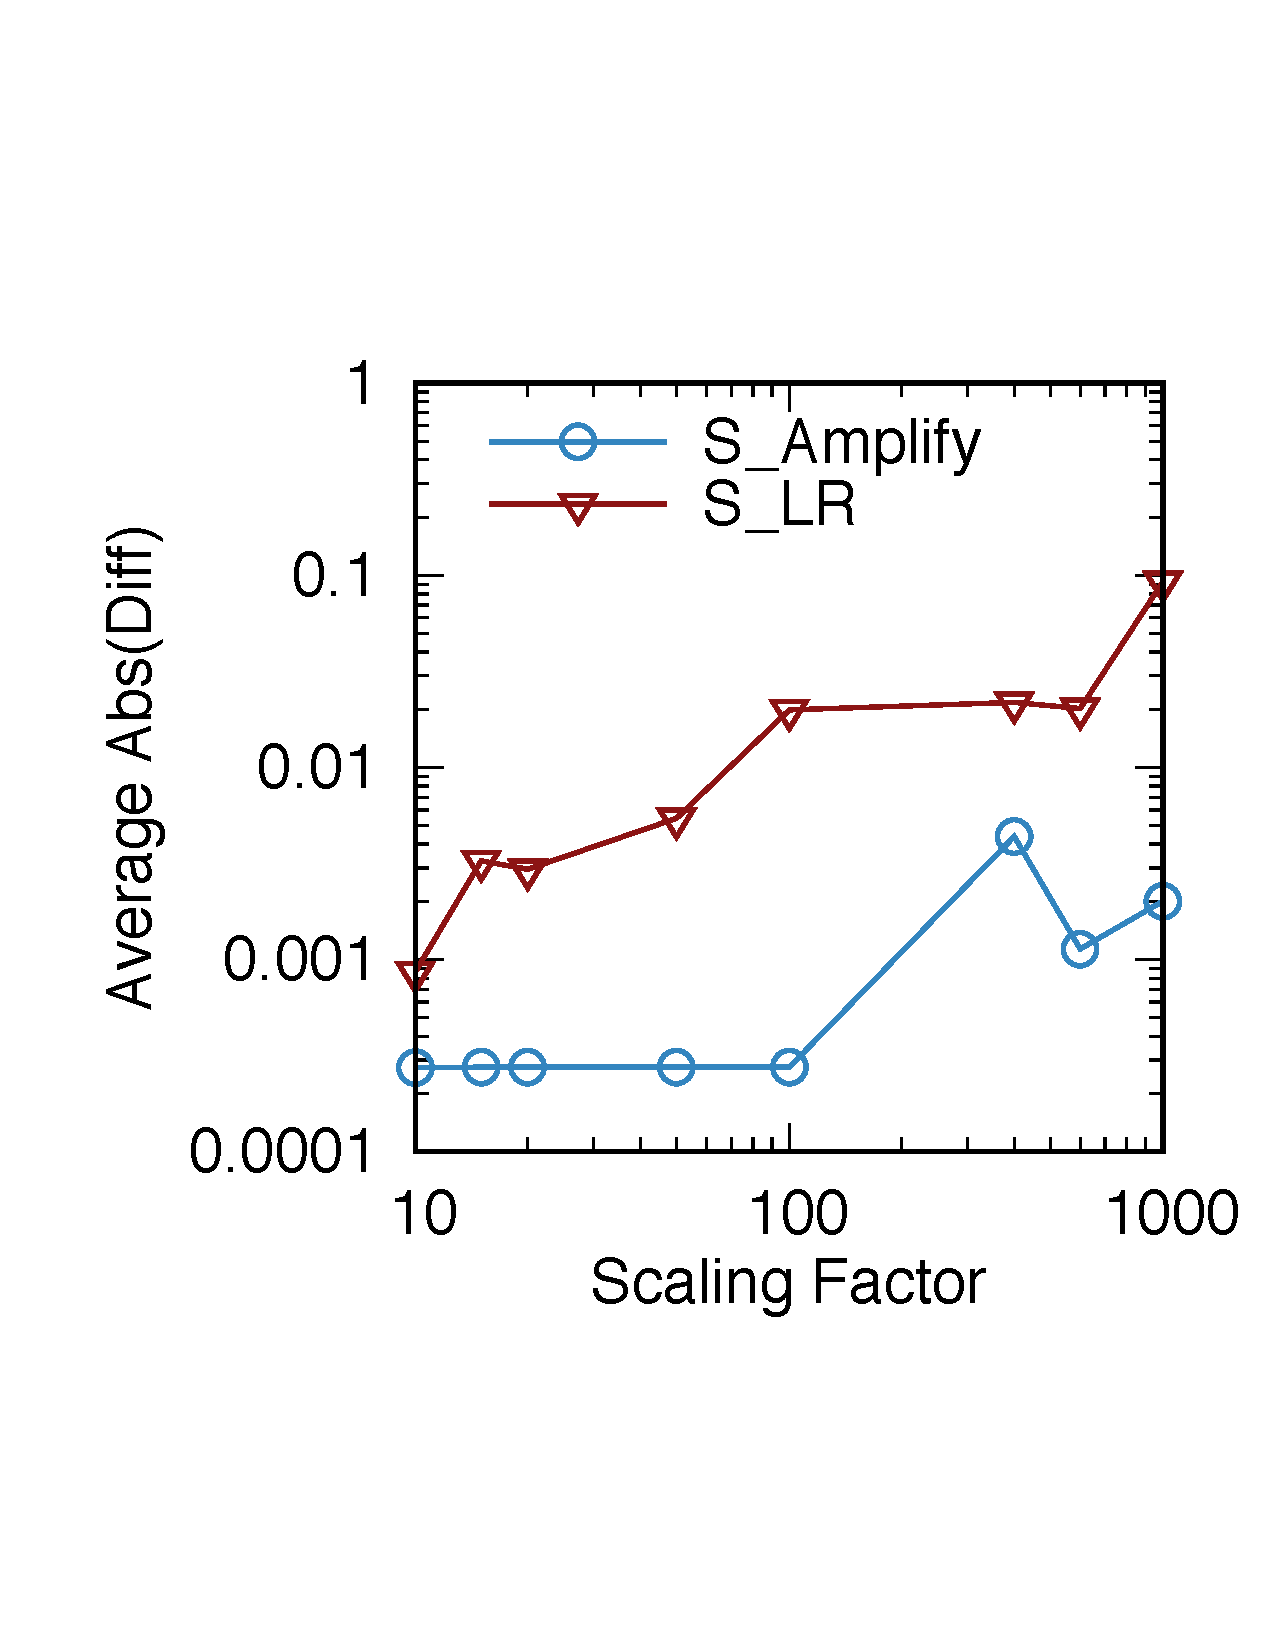
\includegraphics[width=.8\linewidth]{Graph/negSamp/AmplifyLRTheoryL1New.pdf}

		\captionof{figure}{Amplifying factor vs learning rate}
		\label{fig:amplifyLR}
	\end{minipage}%

\end{figure*}



% \begin{figure}[ht]
% 	\centering
% 	\begin{minipage}{.33\textwidth}
% 		\centering
% 		\captionsetup{justification=centering,margin=0.1cm}
% 		\includegraphics[width=.95\linewidth]{Graph/L2Theory_Step.pdf}
% 		\captionof{figure}{Model accuracy}
% 		\label{fig:l2Loss}
% 	\end{minipage}%
% 	\begin{minipage}{.33\textwidth}
% 		\centering
% 		\captionsetup{justification=centering,margin=0.1cm}
% 		\includegraphics[width=.95\linewidth]{Graph/theoryTime.pdf}
% 		\captionof{figure}{Training time.}
% 		\label{fig:trainingTime}
% 	\end{minipage}%
% 	\begin{minipage}{.33\textwidth}
% 		\captionsetup{justification=centering,margin=0.1cm}
% 		\centering
% 		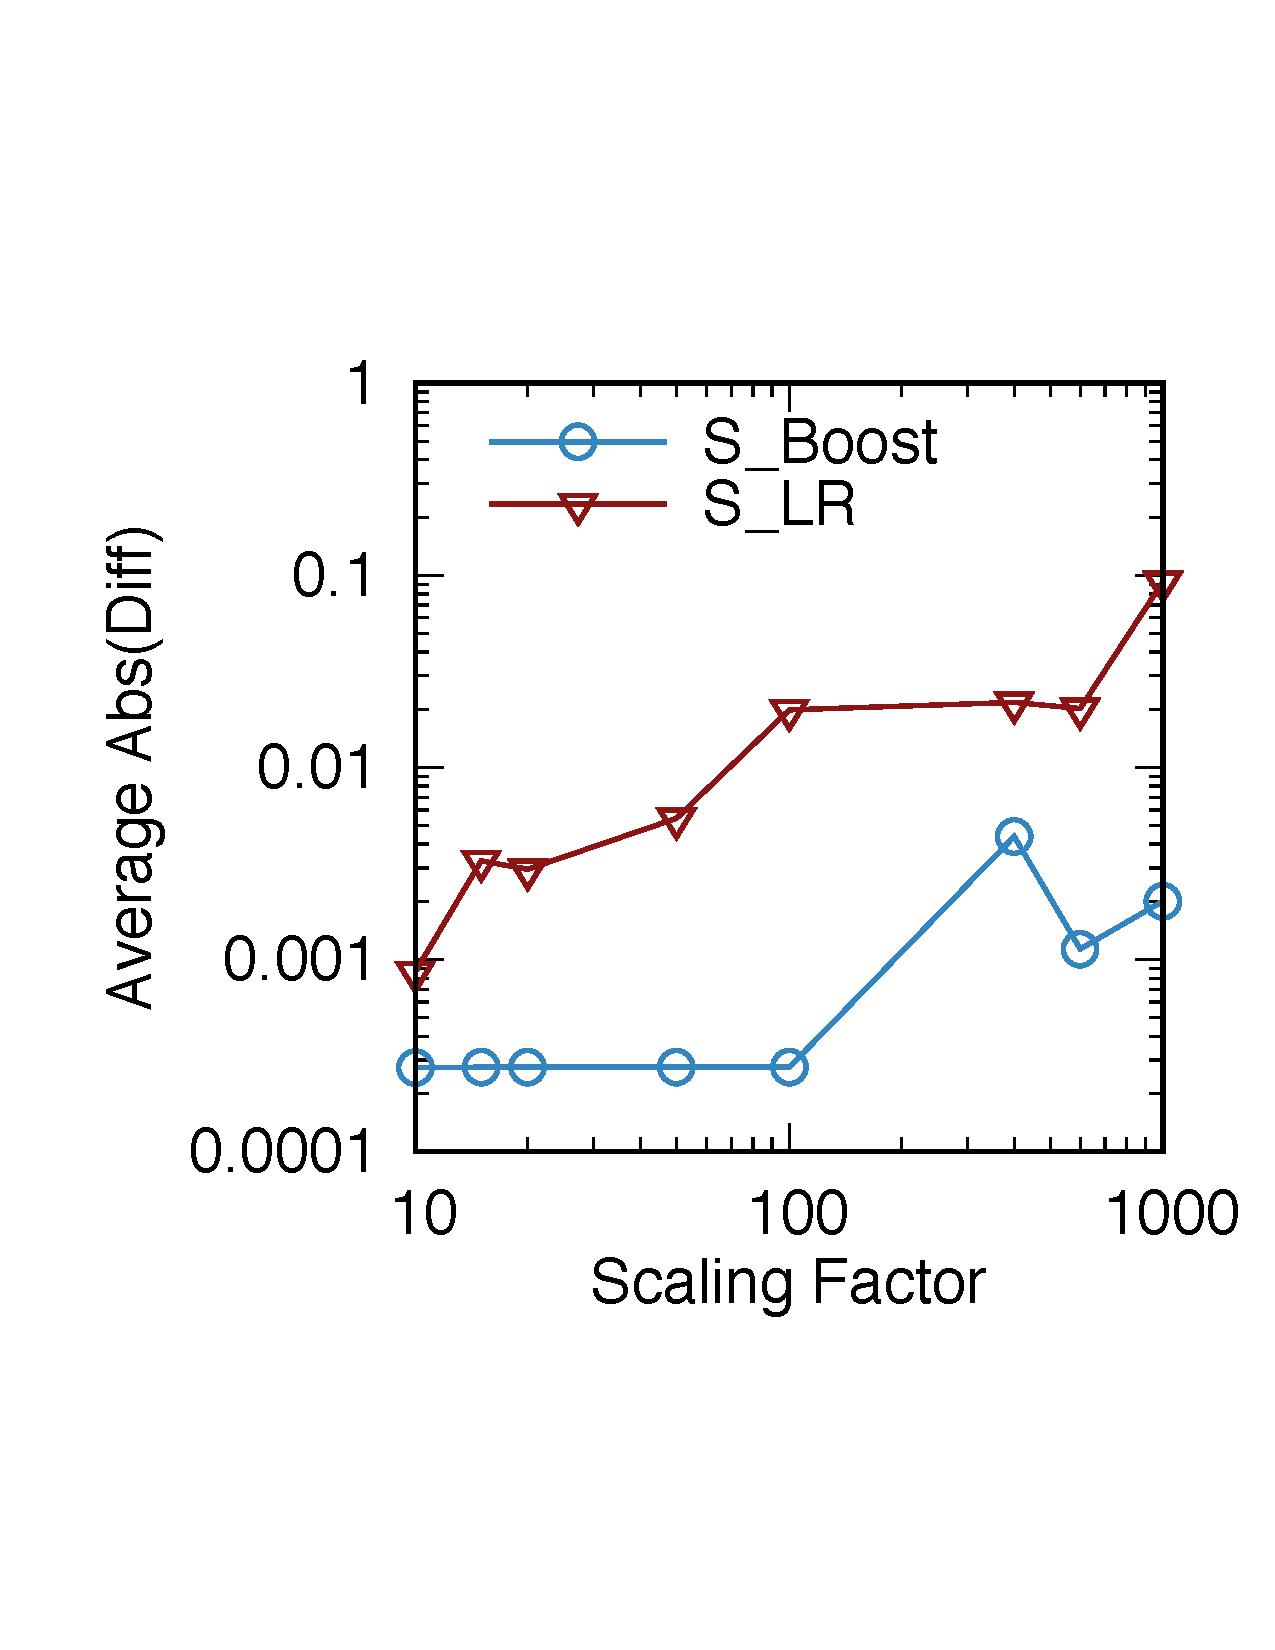
\includegraphics[width=.95\linewidth]{Graph/AmplifyLRTheoryL1New_1.pdf}
% 		\captionof{figure}{Amplifying factor vs learning rate}
% 		\label{fig:amplifyLR}
% 	\end{minipage}%
% 	%
% \end{figure}

\textbf{Model Accuracy and Convergence Rate.} 
In Figure~\ref{fig:l2Loss}, we compare the model accuracy and convergence rate when the model is trained with the four algorithms (FullGrad, Neg5, Neg5-Amplify3, Neg15) under the $L2$ loss function.\footnote{While we performed experiments under all three loss functions, we report the results only from $L2$ here due to space limit. The conclusions from other loss functions are essentially the same.} In the graph, the horizontal axis corresponds to the stochastic-gradient-descent training batch steps (with roughly 70 steps corresponding to one training epoch) and the vertical axis corresponds to the average absolute difference between the trained model $f_{\theta^*}(x, y)$ and MLE $\tilde{P}(y|x) = \frac{\#(x,y)}{\#(x)}$, i.e., $\sum_{(x,y)\in D} \frac{1}{\vert D\vert}\left\vert f_{\theta^*}(x, y) - \frac{\#(x,y)}{\#(x)}\right\vert$. 

From the graph, a few things are clear: (1) Full-gradient training converges to MLE. Even at epoch 1 (step 70), the mean absolute difference of \emph{FullGrad} is close to zero, indicating that it converged to MLE. (2) The amplifying factor $\beta$ effectively ``increases'' the negative sample size by the factor $\beta$ in terms of model accuracy. The mean absolute difference of Neg5-Amplify3 and Neg15 are the same at every training step --- they overlap so closely and it is difficult to tell them apart in the graph --- indicating that they both converge to the same model at the same rate. This result is what our theoretical analysis predicts: $(k=15, \beta = 1)$ leads to the same optimal model as $(k=5, \beta=3)$. (3) A model trained on larger $k$ approximates MLE better. The mean absolute difference of Neg15 is significantly smaller than that of Neg5. 

\textbf{Training Time and Computational Cost.} In Figure~\ref{fig:trainingTime}, we compare the training time of the four algorithms. The horizontal axis corresponds to training epochs and the vertical axis corresponds to training time, which roughly captures the computational cost of each algorithm. The vertical axis is logarithmic; since the training time of \emph{FullGrad} is two orders of magnitude larger than others, its result is not visible in the same graph otherwise. From the graph, we again observe what is predicted by our analysis. The training time of Neg5-Amplify3 is practically the same as that of Neg5. That is, Neg5-Amplify3 works almost like Neg5 in terms of its training time and computational cost, but it works almost like  Neg15 in terms of its model accuracy and convergence rate! Amplified negative sampling indeed gives the best of both worlds.

\textbf{Learning Rate vs Amplifying Factor.} In Figure~\ref{fig:amplifyLR}, we compare the effect of using different learning rates and amplifying factors. The graph is from training the model using Neg15 under $L1$ loss. The curve labeled as \emph{S\_LR} is obtained by multiplying the default learning rate of 0.025 by a factor between 10 and 1,000. The curve labeled as \emph{S\_Amplify} is obtained by including the amplifying factor $\beta$ between 10 and 1,000. The vertical axis is again in the logarithmic scale due to the high difference between the two curves and represents the model accuracy (the mean absolute difference from MLE) at the given learning rate/amplifying factor. From the graph, we see that changing the learning rate and changing the amplifying factor lead to vastly different results. As we increase the learning rate, the trained model diverges further away from MLE. When we increase the amplifying factor, however, the trained model stays close to MLE all the way through $\beta = 100$. Only after $\beta > 100$, the model starts to diverge and becomes unstable. This result is consistent with our analysis; according to Corollary~\ref{th:amplified}, amplifying converges to MLE at $\beta \approx 140$ under the current setting,\footnote{Amplified negative sampling converges to MLE when $\beta k p_y = 1$. Given $k=15$ and the uniform probability $p_y \approx 1/2000$ for this experiment, $\beta k p_y = 1$ at $\beta \approx 140$.} so its divergence beyond $\beta > 140$ is expected.

%\subsection{Language Model perplexity test}
%In this section, Amplified Negative Sampling method is tested on the Language Model on Penn Tree Bank(PTB) dataset~\citep{marcus-etal-1993-building} to demonstrate its performance. We use one of the commonly tested RNN Language model~\citep{zaremba2014recurrent} with the medium regularized settings as in ~\citep{blanc2017adaptive}. The PTB dataset contains 929K training words, 73k validation and 82k test words. We keep the original settings of the RNN model and set the hidden dimension as 650.
%
%The perplexity result is reported in Figure \ref{fig:neg5} and \ref{fig:neg15} for Neg5 and Neg15 experiment. For each negative sample setting, the amplifying factor is set to 1, 3 and 10 respectively. As the amplifying factor got enlarged, the perplexity got decreased. Every experiment converges in around 20 epochs.
%As shown in figure \ref{fig:neg5}, the amplifying factor can effectively decrease the perplexity compared with other model when only a few number of samples are allowed. Here the result is drawn from ~\citep{blanc2017adaptive} to demonstrate the Neg5 result with amplifying factor 10 can compete with ~\citep{blanc2017adaptive}'s 10 sample result.
%
%Further experiments are made on the effect of the amplifying factor. As shown in Figure \ref{fig:factor}, when the amplifying factor is increased from 1, the perplexity have a clear decrease until 10 and the perplexity starts to increase when the amplifying factor keeps enlarging. The best model performance will be obtained when the amplifying factor is configured around 10. An explanation based on formula (\ref{eq:amplifyed}) is the convergence condition is $t$(epoch) tends to infinity. However, in experiment, the training process will be stopped as the performance doesn't change anymore or the model got trapped in the saddle point. In this case, the model won't converge to the optimum value and a large amplifying factor will also change the convergence point to a non-optimum point.
%
%
%
%
%\begin{figure*}[ht]
%	\centering
%	\begin{minipage}{.31\textwidth}
%		\centering
%		\captionsetup{justification=centering,margin=0.1cm}
%		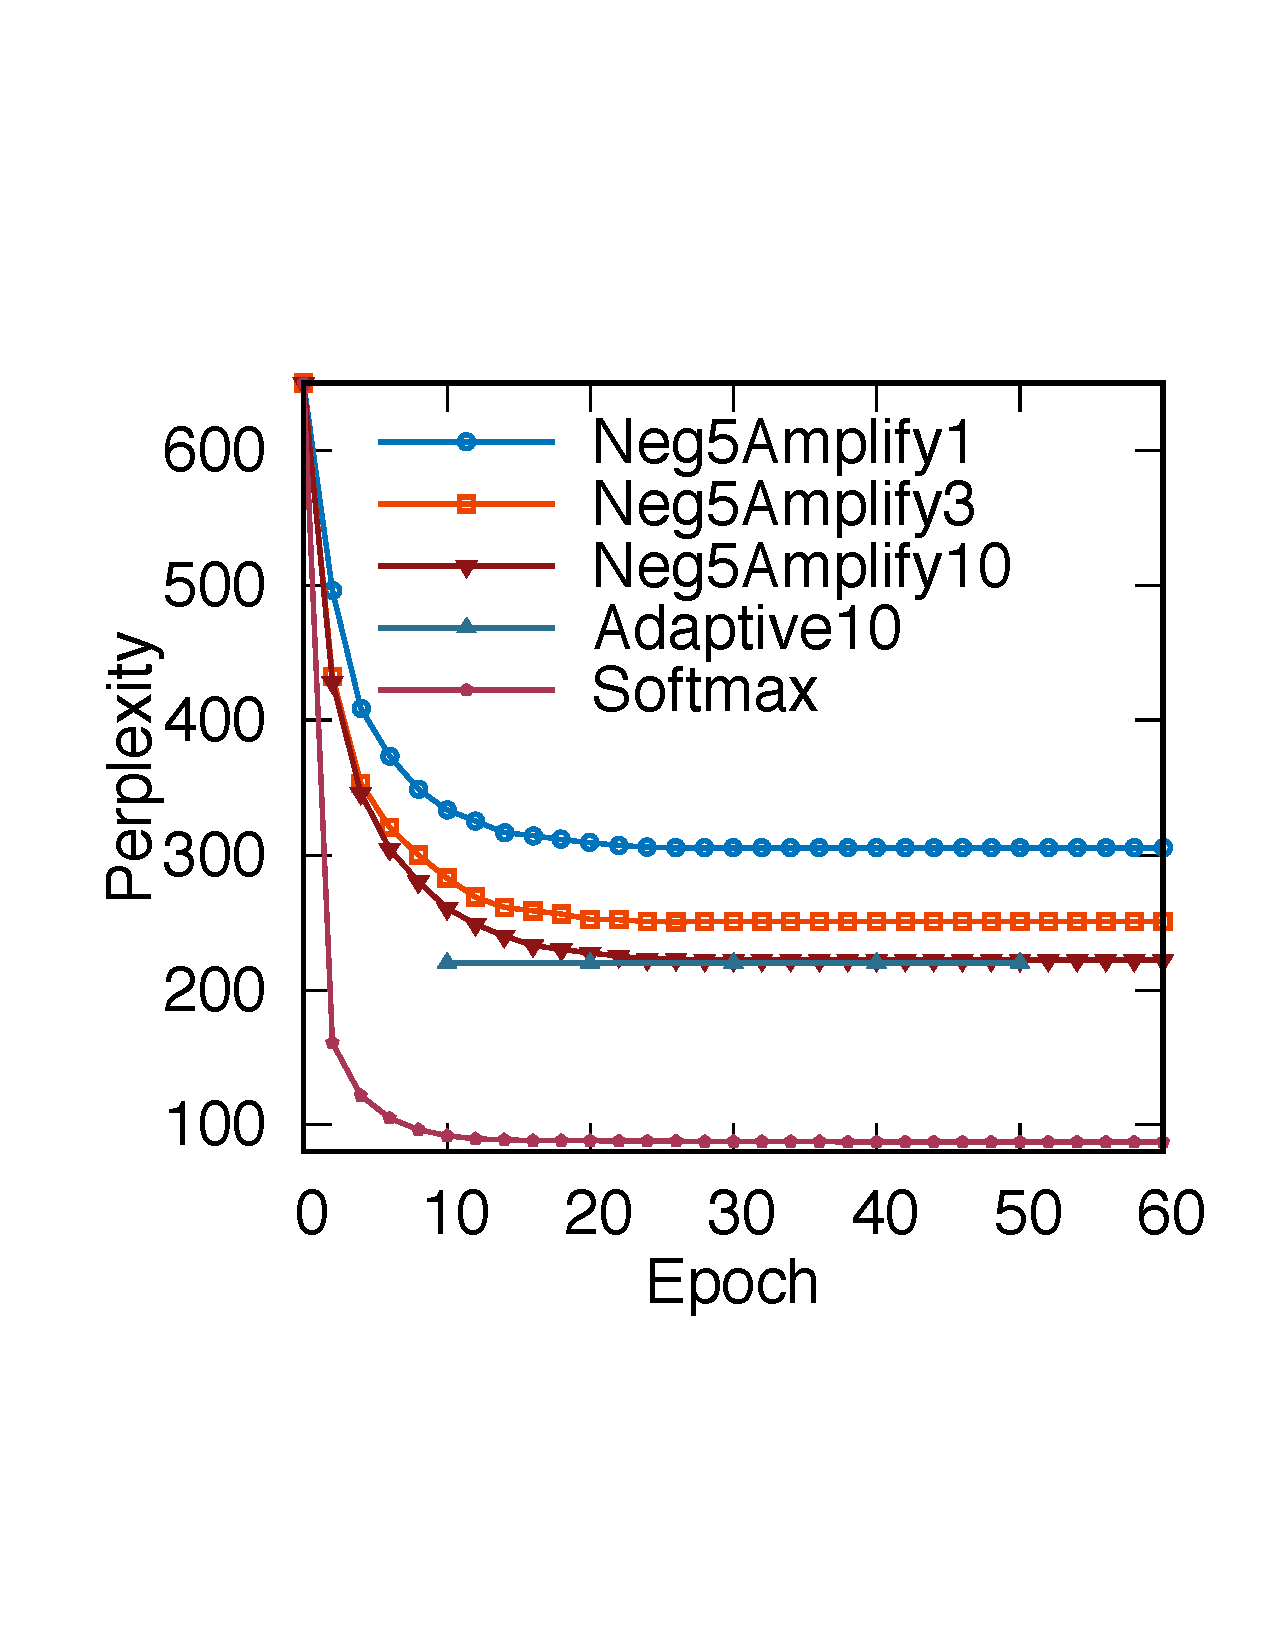
\includegraphics[width=1\linewidth]{Graph/negSamp/L2Neg5_60_Nolog.pdf}
%
%		\captionof{figure}{PTB: Negative sampling 5.}
%		\label{fig:neg5}
%	\end{minipage}%
%	\begin{minipage}{.31\textwidth}
%		\centering
%		\captionsetup{justification=centering,margin=0.1cm}
%		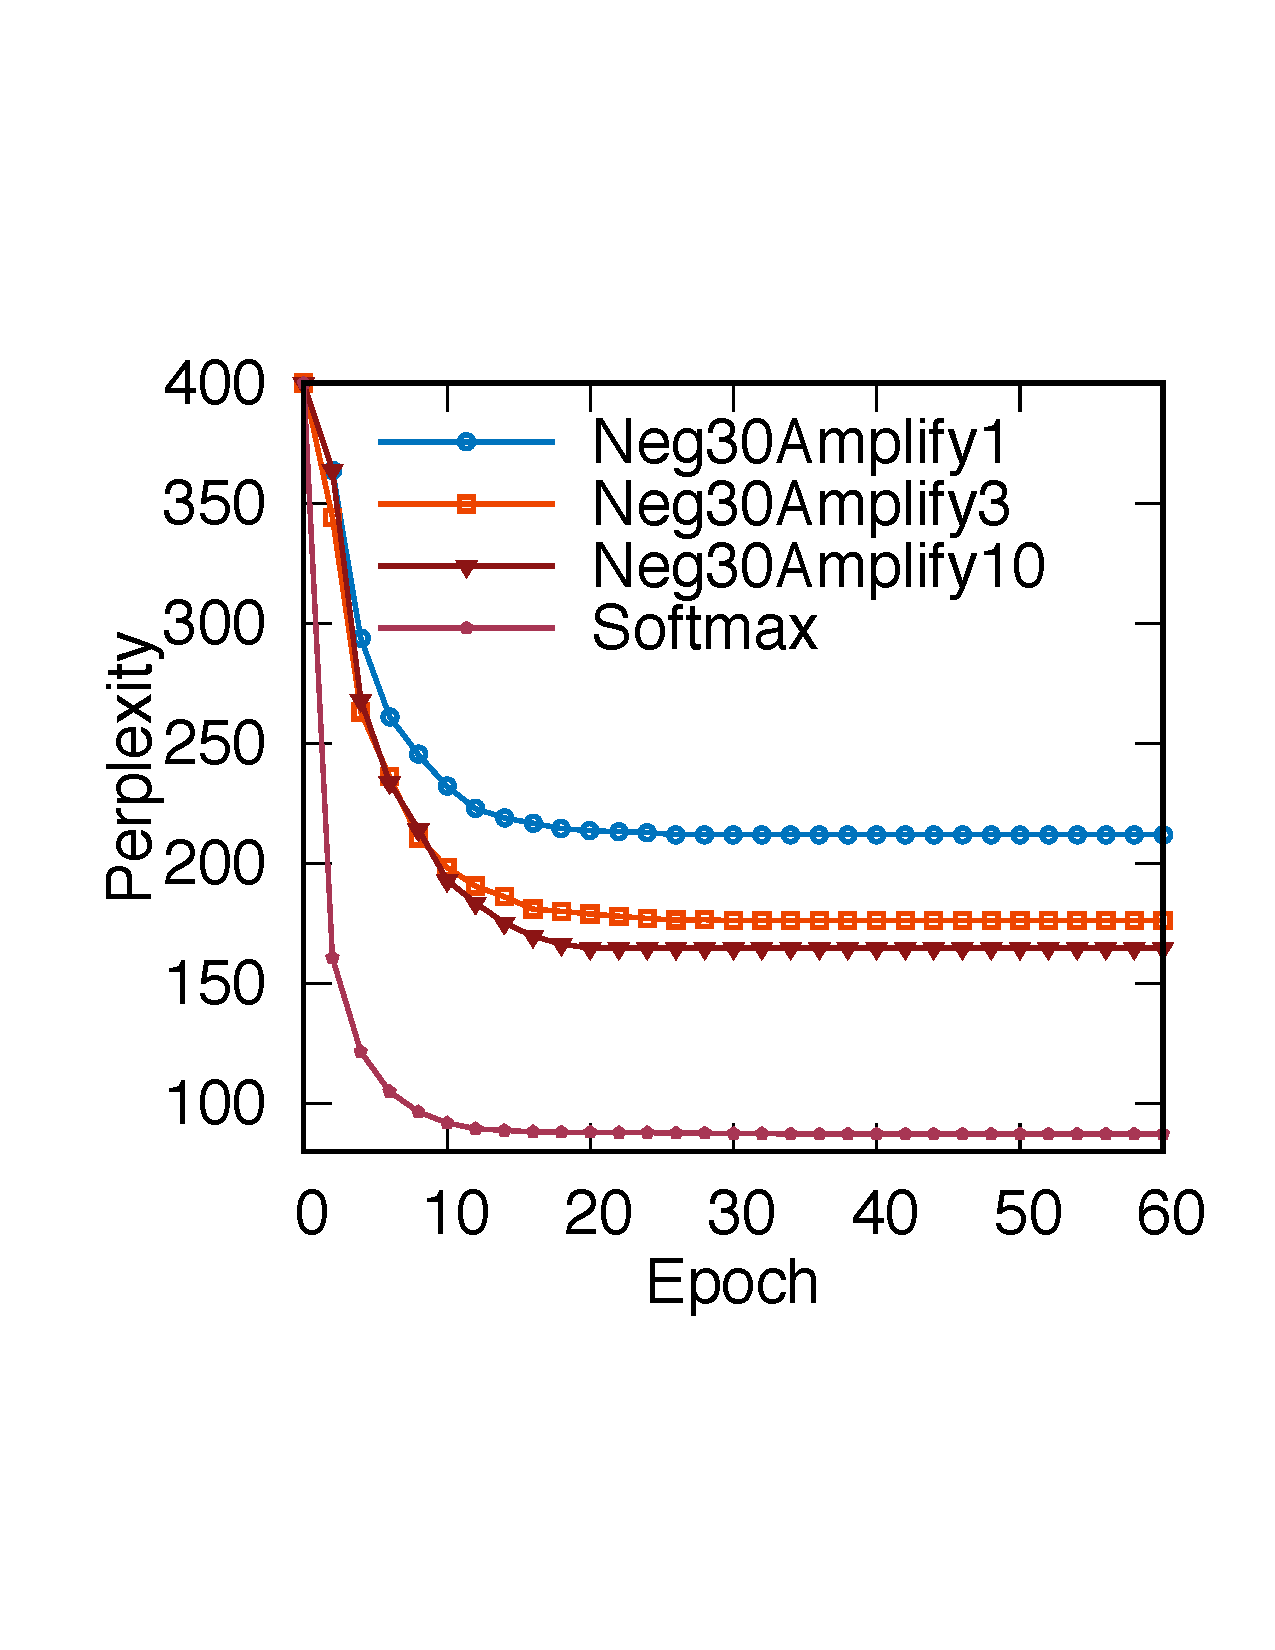
\includegraphics[width=1\linewidth]{Graph/negSamp/L2Neg30_60_Nolog.pdf}
%
%		\captionof{figure}{PTB: Negative sampling 15.}
%		\label{fig:neg15}
%	\end{minipage}%
%	\begin{minipage}{.38\textwidth}
%		\captionsetup{justification=centering,margin=0.1cm}
%		\centering
%		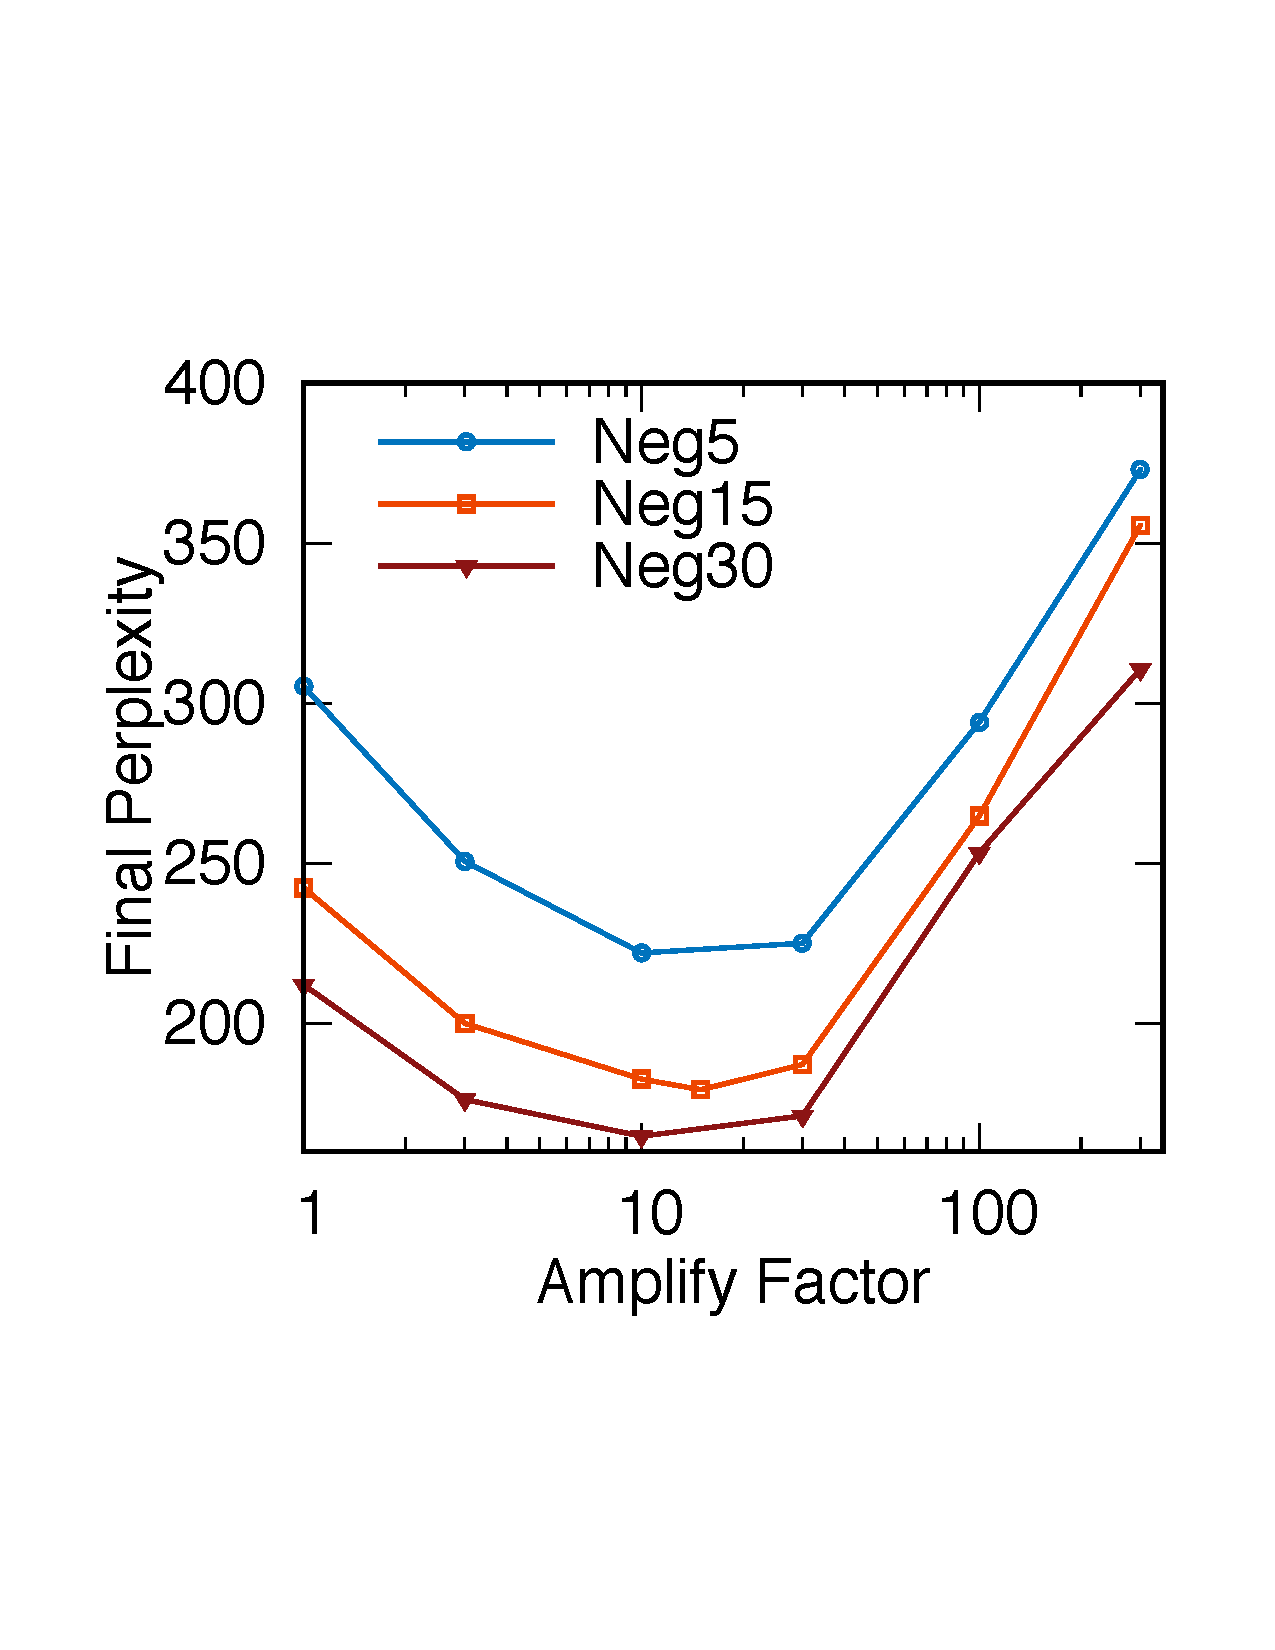
\includegraphics[width=.8\linewidth]{Graph/negSamp/L2NegAllAmplify.pdf}
%
%		\captionof{figure}{Different amplifying factor.}
%		\label{fig:factor}
%	\end{minipage}%
%
%\end{figure*}

\subsection{Experiments on Other Downstream Tasks}\label{sec:realworld}
In the previous set of experiments, we investigated the effect of amplified negative sampling on the trained model in terms of its difference from MLE. In the next set of experiments, we investigate its effect on three other downstream tasks: (a) word-analogy tasks (b) rare-word-similarity tasks and (c) graph-node-classification tasks. In all our experiments, we compare the results from Neg5, Neg5-Amplify3, and Neg15 at training epoch 3. 

\textbf{Word2vec: Word analogy.} This test is conducted with the CBOW model trained on the Text8 corpus~~\citep{mikolov2013distributed} using the code downloaded from ~\citep{word2vecGithub} after we add amplifying code. The performance is evaluated by the 14 word-analogy tasks in~~\citep{mikolov2013distributed}. We use the default parameter settings of the downloaded code.

\textbf{Fasttext: Rare word similarity.}
For the word-similarity task, we use the code for Fasttext ~\citep{fastText} downloaded from~~\citep{fastTextGithub} using its default settings after the addition of amplifying code. The model is trained on the rare word dataset (RW)~~\citep{luong2013better}. The effectiveness of a trained model is measured by the Spearman’s rank-correlation coefficient~~\citep{spearman1904proof} between the human judgment in the dataset and the output from the trained model.

\textbf{Node2vec: Node classification.} For the node classification task, we use the node2vec model ~\citep{node2vec-kdd2016} with the code downloaded from ~\citep{node2vecGithub}. The dataset used is BlogCatalog ~\citep{Zafarani+Liu:2009}. The nodes are embedded into a 50-dimensional space and we use 20-80 train-test split. The default parameter setting of the downloaded code is used after the addition of amplifying code.   

In Table~\ref{tbl:semantic} we show the accuracy of Neg5, Neg5-Amplify3, and Neg15 for the first 5 word-analogy semantic tasks of~~\citep{mikolov2013distributed}. From the results, the trend is clear: the performance of Neg5-Amplify3 is higher than Neg5 and is close to Neg15. In Table~\ref{tbl:time}, we show the training times of Word2vec, Fasttext, and Node2vec. In all three cases, the training time of Neg5-Amplify is close to Neg5 and is significantly smaller than that of Neg15. In the cases of Fasttext and Word2vec, the difference is by a factor 2. In the case of Node2vec, the difference is much smaller due to the dominance of other training overhead when the absolute training time is small.
From our other experiments whose results we could not include here due to space limit, we observe the same general trend: The downstream-task performance of Neg5-Amplify3 is close to Neg15 while its training cost is close to Neg5. 

\vspace{2em}
\makebox[\linewidth][c]{
\begin{minipage}{1\textwidth}
	%\begin{table}[h]
	
	\captionof{table}{Word-analogy semantic-task top-1 accuracy.}
	\label{tbl:semantic}
		\centering
		\begin{tabular}{| c |c c c|} 

			\hline
			Task Name & Neg5 & Neg5-Amplify3 & Neg15 \\
			\hline
			capital-common-countries & 38.14 & 43.02 & 47.43\\
			capital-world & 24.66 & 29.34 & 32.14\\
			city-in-state & 15.17 & 17.29 & 14.93\\
			currency & 15.72 & 22.26 & 22.21\\
			family & 56.86 & 60.30 & 64.27\\
			\hline
	\end{tabular}
\end{minipage}}
\vspace{2em}

% \begin{minipage}{.49\textwidth}
% %\begin{table}[h]

% \captionof{table}{Word-analogy semantic-task top-1 accuracy.}
% \label{tbl:semantic}
% \scalebox{0.8}{
%  \begin{tabular}{| c |c c c c c|} 
%  \hline

% Algorithm    &Task 1 & Task 2 & Task 3 & Task 4 & Task 5 \\
% \hline
% %  Neg5& 		37.15 &  23.21 &  14.55 &  16.42 &  52.94 \\

% %  Neg5-Amplify3& 42.29 &  27.2 &  14.18 &  22.02 &  58.5\\

% %  Neg15& 		47.04 &  31.47 &  16.04 &  22.15 &  65.69  \\
%  Neg5& 		38.14 &  24.66 &  15.17 &  15.72 &  56.86 \\

%  Neg5-Amplify3& 43.02 &  29.34 &  17.29 &  22.26 &  60.30\\

%  Neg15& 		47.43 &  32.14 &  14.93 &  22.21 &  64.27  \\


% \hline
% \end{tabular}}
% \vspace{3ex}
% 	\end{minipage}%
% 	\quad\quad%
% \begin{minipage}{0.49\textwidth}
%   \vspace{1.5ex}
% \captionof{table}{Mapping from Task ID to task real name for word analogy semantic-task.}
% \label{tbl:semanticName}
% \centering
% \scalebox{0.8}{
% \begin{tabular}{|c | c|} 
%  \hline

% Task ID & Real Name   \\
% \hline
% 1&	capital-common-countries\\
% 2&	capital-world\\
% 3&	city-in-state\\
% 4&	currency\\
% 5&	family\\
% % 6&	gram1-adjective-to-adverb\\
% % 7&	gram2-opposite\\
% % 8&	gram3-comparative\\
% % 9&	gram4-superlative\\
% % 10&	gram5-present-participle\\
% % 11&	gram6-nationality-adjective\\
% % 12&	gram7-past-tense\\
% % 13&	gram8-plural\\
% % 14&	gram9-plural-verbs\\

% \hline
% \end{tabular}}

% \end{minipage}

%\begin{minipage}{\textwidth}


\makebox[\linewidth][c]{
\begin{minipage}{1\textwidth}
	\captionof{table}{Training time (seconds).}
	\label{tbl:time}	
		\centering
		\begin{tabular}{|c|c c c|} 
		
			\hline
			Model & Neg5 &Neg5-Amplify3 & Neg15\\
			\hline
			Fasttext&736&731&1404\\
			Word2vec&17.35&17.37&36.93\\
			Node2vec&3.28&3.28 &4.00\\
			\hline
	\end{tabular}
	%   \captionof{table}{Training time (seconds).}
	% \label{tbl:time}
\end{minipage}}
%\end{minipage}
% \section{Experiments}\label{sec:experiments}
% The primary goal of this section is to experimentally investigate the following two issues: (1) Does the result of our analysis hold in practice? We want to examine how well our theoretical results match with experiments. We also want to experimentally explore a few questions raised in this chapter, including the choice of the optimal amplifying factor and the difference between the learning rate and the amplifying factor. (2) Does amplified negative sampling help other downstream tasks as well? The performance of other downstream tasks may not necessarily depend on how accurately the trained model captures the conditional probability $P(y|x)$, so we want to experimentally check whether amplified negative sampling has positive effects on other downstream tasks or not. 

% In the subsection (Model Accuracy and Training Efficiency)~\ref{sec:simulation}, we explore the first issue by measuring the difference between the maximum likelihood estimator (MLE) $\tilde{P}(y|x) = \frac{\#(x,y)}{\#(x)}$ and the models trained with (a) full-gradient training (b) negative sampling and (c) amplified negative sampling. The results of our experiments show that the conclusions of our analysis hold in practice to a surprising degree of accuracy. They also show that the learning rate and the amplifying factor have vastly different effects on the trained model. In the subsection (Experiments on Other Downstream Tasks)~\ref{sec:realworld}, we investigate the second issue by running experiments on three different downstream tasks: word-analogy tasks~~\citep{mikolov2013efficient}, rare-word-similarity tasks~~\citep{fastText}, and graph-node-classification tasks~~\citep{node2vec-kdd2016}. Here, we observe that amplified negative sampling leads to improved performance on these  downstream tasks as well. 


% In summary, our experimental results strongly indicate that there really is not much downside to using amplified negative sampling; as long as we use a reasonably small amplifying factor, say $\beta = 3$, amplified negative sampling leads to lower training time and higher model accuracy.

% \subsection{Model Accuracy and Training Efficiency}\label{sec:simulation}

% \textbf{Experimental Settings.} 
% In this subsection, we experimentally compare four training algorithms, full-gradient training (\textit{FullGrad}), 5 negative samples (\textit{Neg5}), 5 negative samples with the amplifying factor 3 (\textit{Neg5-Amplify3}), and 15 negative samples (\textit{Neg15}),
% under three different loss functions, $L1$, $L2$, and cross entropy. For the choice of the hypothesis space $f_{\theta}(x,y)$ and the training set, we use a setting similar to~~\citep{mikolov2013efficient}. That is, as our hypothesis space we use the skip-gram model of~~\citep{mikolov2013efficient} with a 100-dimensional hidden layer.
% As our dataset, we use a subset of Text8 corpus from~~\citep{mikolov2013efficient} by extracting the first 75,000 words and applying the same min\_count filter of 5 in~~\citep{mikolov2013efficient}.\footnote{Using a subset of Text8 here is due to the high training cost of \textit{FullGrad} and our desire to keep the training time at a manageable level. In our next experiments on other downstream tasks, we run report our results from experiments on much larger datasets.} We use the stochastic-gradient descent (SGD) with the batch size of 500 as the training algorithm. All our experiments use the window size 3 and the learning rate 0.025 unless noted otherwise. All other parameter settings are the same as in~~\citep{mikolov2013efficient}. All results reported are the average of three independent runs with identical settings. All codes were implemented using PyTorch v1.0.1. 

% \begin{figure*}[ht]
% 	\centering
% 	\begin{minipage}{.31\textwidth}
% 		\centering
% 		\captionsetup{justification=centering,margin=0.1cm}
% 		\includegraphics[width=1\linewidth]{Graph/L2Theory_Step.pdf}
% 		\vspace{-13ex}
% 		\captionof{figure}{Model accuracy.}
% 		\label{fig:l2Loss}
% 	\end{minipage}%
% 	\begin{minipage}{.31\textwidth}
% 		\centering
% 		\captionsetup{justification=centering,margin=0.1cm}
% 		\includegraphics[width=1\linewidth]{Graph/theoryTime.pdf}
% 		\vspace{-13ex}
% 		\captionof{figure}{Training time.}
% 		\label{fig:trainingTime}
% 	\end{minipage}%
% 	\begin{minipage}{.38\textwidth}
% 		\captionsetup{justification=centering,margin=0.1cm}
% 		\centering
% 		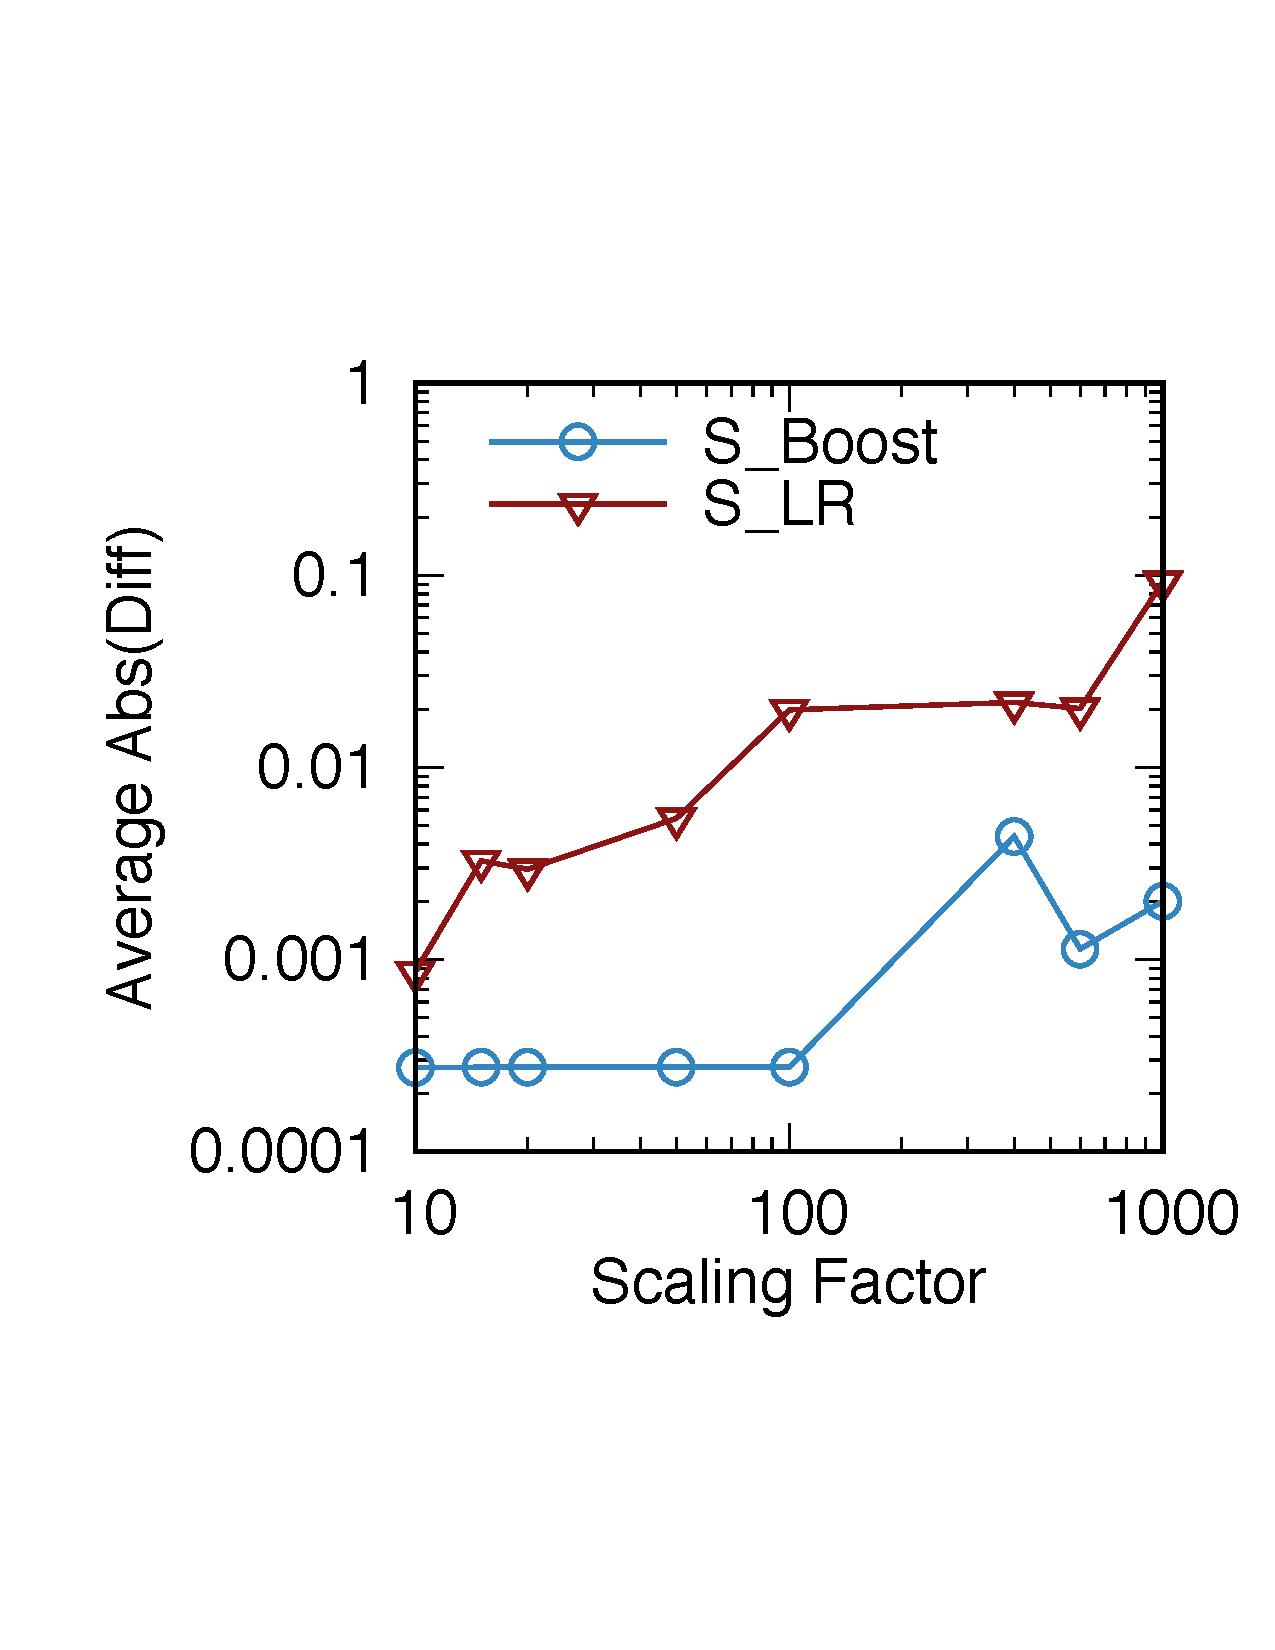
\includegraphics[width=.8\linewidth]{Graph/AmplifyLRTheoryL1New_1.pdf}
% 		\vspace{-10ex}
% 		\captionof{figure}{Amplifying factor vs learning rate.}
% 		\label{fig:amplifyLR}
% 	\end{minipage}%
% 	\vspace{-1.5em}
% \end{figure*}



% % \begin{figure}[ht]
% % 	\centering
% % 	\begin{minipage}{.33\textwidth}
% % 		\centering
% % 		\captionsetup{justification=centering,margin=0.1cm}
% % 		\includegraphics[width=.95\linewidth]{Graph/L2Theory_Step.pdf}
% % 		\captionof{figure}{Model accuracy}
% % 		\label{fig:l2Loss}
% % 	\end{minipage}%
% % 	\begin{minipage}{.33\textwidth}
% % 		\centering
% % 		\captionsetup{justification=centering,margin=0.1cm}
% % 		\includegraphics[width=.95\linewidth]{Graph/theoryTime.pdf}
% % 		\captionof{figure}{Training time.}
% % 		\label{fig:trainingTime}
% % 	\end{minipage}%
% % 	\begin{minipage}{.33\textwidth}
% % 		\captionsetup{justification=centering,margin=0.1cm}
% % 		\centering
% % 		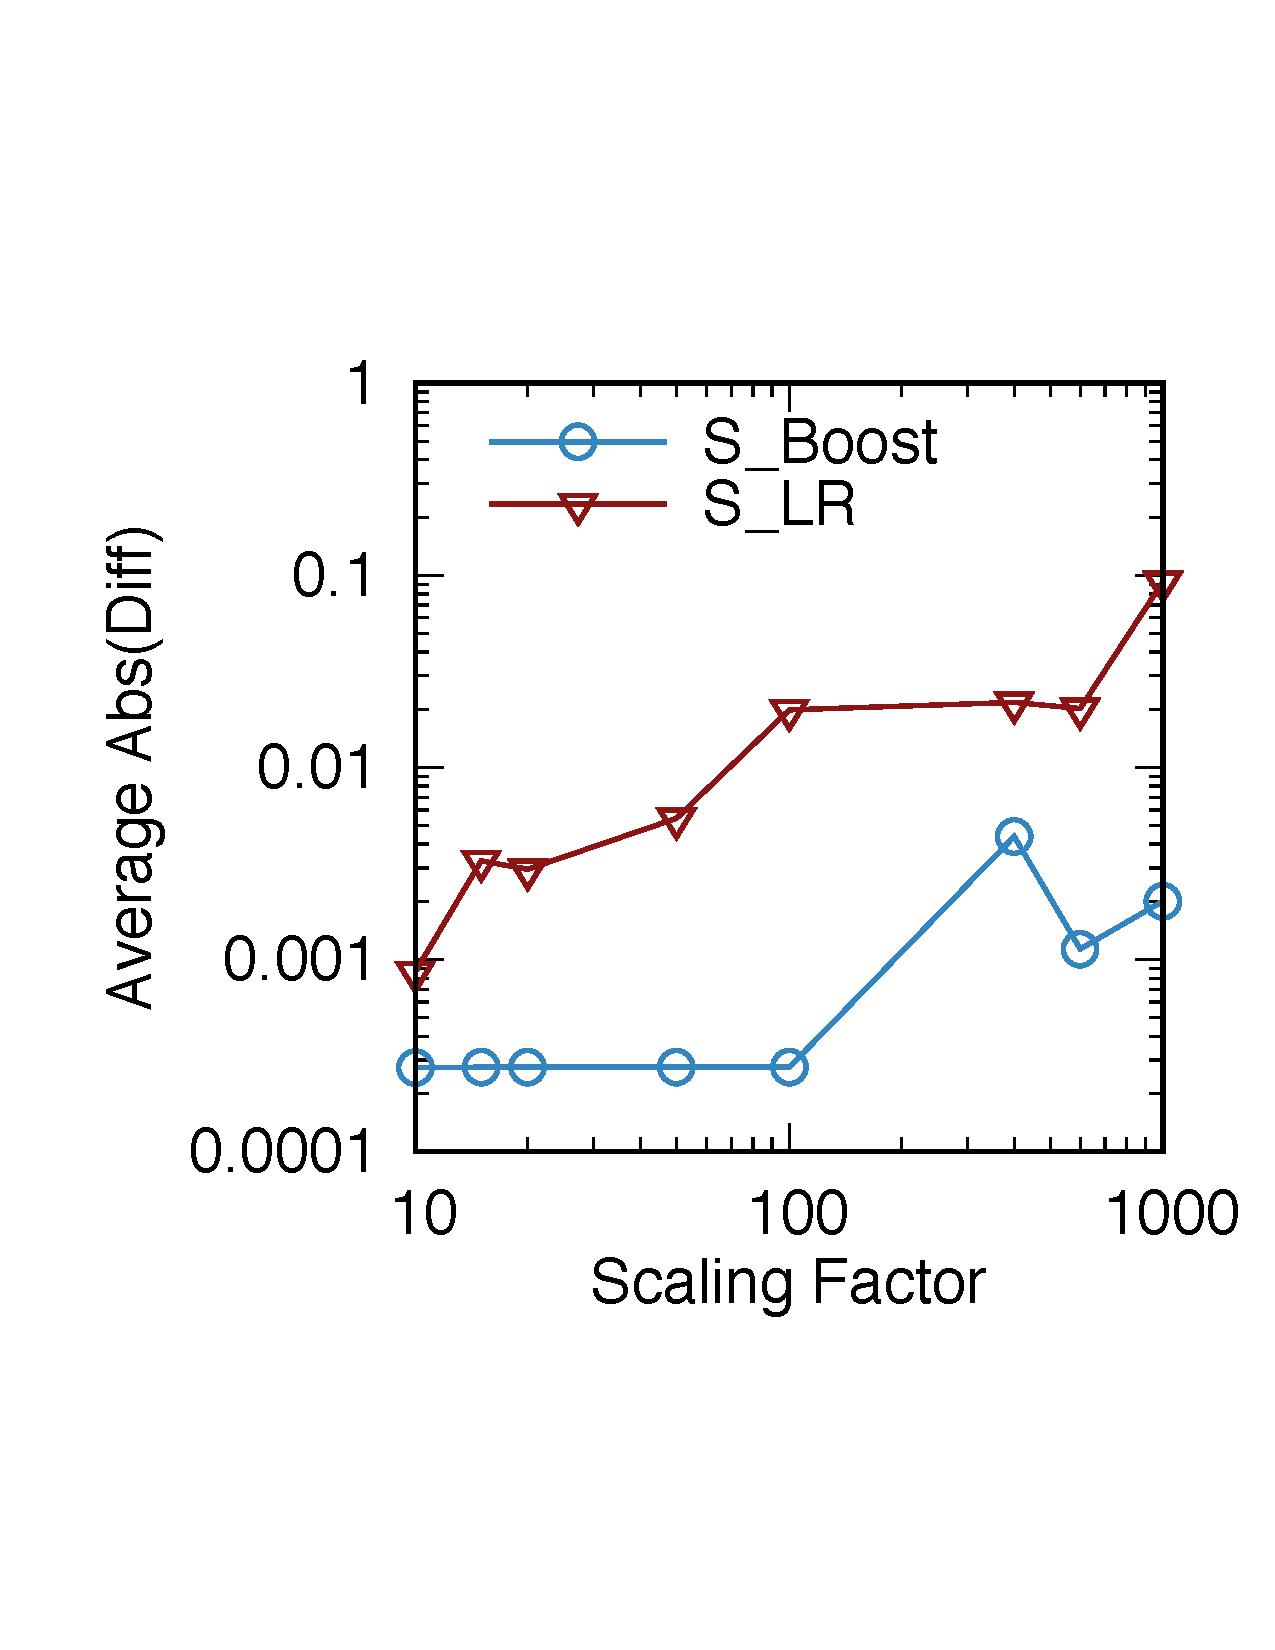
\includegraphics[width=.95\linewidth]{Graph/AmplifyLRTheoryL1New_1.pdf}
% % 		\captionof{figure}{Amplifying factor vs learning rate}
% % 		\label{fig:amplifyLR}
% % 	\end{minipage}%
% % 	%
% % \end{figure}

% \textbf{Model Accuracy and Convergence Rate.} 
% In Figure~\ref{fig:l2Loss}, we compare the model accuracy and convergence rate when the model is trained with the four algorithms (FullGrad, Neg5, Neg5-Amplify3, Neg15) under the $L2$ loss function.\footnote{While we performed experiments under all three loss functions, we report the results only from $L2$ here due to space limit. The conclusions from other loss functions are essentially the same.} In the graph, the horizontal axis corresponds to the stochastic-gradient-descent training batch steps (with roughly 70 steps corresponding to one training epoch) and the vertical axis corresponds to the average absolute difference between the trained model $f_{\theta^*}(x, y)$ and MLE $\tilde{P}(y|x) = \frac{\#(x,y)}{\#(x)}$, i.e., $\sum_{(x,y)\in D} \frac{1}{\vert D\vert}\left\vert f_{\theta^*}(x, y) - \frac{\#(x,y)}{\#(x)}\right\vert$. 

% From the graph, a few things are clear: (1) Full-gradient training converges to MLE. Even at epoch 1 (step 70), the mean absolute difference of \emph{FullGrad} is close to zero, indicating that it converged to MLE. (2) The amplifying factor $\beta$ effectively ``increases'' the negative sample size by the factor $\beta$ in terms of model accuracy. The mean absolute difference of Neg5-Amplify3 and Neg15 are the same at every training step --- they overlap so closely and it is difficult to tell them apart in the graph --- indicating that they both converge to the same model at the same rate. This result is what our theoretical analysis predicts: $(k=15, \beta = 1)$ leads to the same optimal model as $(k=5, \beta=3)$. (3) A model trained on larger $k$ approximates MLE better. The mean absolute difference of Neg15 is significantly smaller than that of Neg5. 

% \textbf{Training Time and Computational Cost.} In Figure~\ref{fig:trainingTime}, we compare the training time of the four algorithms. The horizontal axis corresponds to training epochs and the vertical axis corresponds to training time, which roughly captures the computational cost of each algorithm. The vertical axis is logarithmic; since the training time of \emph{FullGrad} is two orders of magnitude larger than others, its result is not visible in the same graph otherwise. From the graph, we again observe what is predicted by our analysis. The training time of Neg5-Amplify3 is practically the same as that of Neg5. That is, Neg5-Amplify3 works almost like Neg5 in terms of its training time and computational cost, but it works almost like  Neg15 in terms of its model accuracy and convergence rate! Amplified negative sampling indeed gives the best of both worlds.

% \textbf{Learning Rate vs Amplifying Factor.} In Figure~\ref{fig:amplifyLR}, we compare the effect of using different learning rates and amplifying factors. The graph is from training the model using Neg15 under $L1$ loss. The curve labeled as \emph{S\_LR} is obtained by multiplying the default learning rate of 0.025 by a factor between 10 and 1,000. The curve labeled as \emph{S\_Amplify} is obtained by including the amplifying factor $\beta$ between 10 and 1,000. The vertical axis is again in the logarithmic scale due to the high difference between the two curves and represents the model accuracy (the mean absolute difference from MLE) at the given learning rate/amplifying factor. From the graph, we see that changing the learning rate and changing the amplifying factor lead to vastly different results. As we increase the learning rate, the trained model diverges further away from MLE. When we increase the amplifying factor, however, the trained model stays close to MLE all the way through $\beta = 100$. Only after $\beta > 100$, the model starts to diverge and becomes unstable. This result is consistent with our analysis; according to Corollary~\ref{th:amplified}, amplifying converges to MLE at $\beta \approx 140$ under the current setting,\footnote{Amplified negative sampling converges to MLE when $\beta k p_y = 1$. Given $k=15$ and the uniform probability $p_y \approx 1/2000$ for this experiment, $\beta k p_y = 1$ at $\beta \approx 140$.} so its divergence beyond $\beta > 140$ is expected.

% \subsection{Experiments on Other Downstream Tasks}\label{sec:realworld}
% In the previous set of experiments, we investigated the effect of amplified negative sampling on the trained model in terms of its difference from MLE. In the next set of experiments, we investigate its effect on three other downstream tasks: (a) word-analogy tasks (b) rare-word-similarity tasks and (c) graph-node-classification tasks. In all our experiments, we compare the results from Neg5, Neg5-Amplify3, and Neg15 at training epoch 3. 

% \textbf{Word2vec: Word analogy.} This test is conducted with the CBOW model trained on the Text8 corpus~~\citep{mikolov2013distributed} using the code downloaded from ~\citep{word2vecGithub} after we add amplifying code. The performance is evaluated by the 14 word-analogy tasks in~~\citep{mikolov2013distributed}. We use the default parameter settings of the downloaded code.

% \textbf{Fasttext: Rare word similarity.}
% For the word-similarity task, we use the code for Fasttext ~\citep{fastText} downloaded from~~\citep{fastTextGithub} using its default settings after the addition of amplifying code. The model is trained on the rare word dataset (RW)~~\citep{luong2013better}. The effectiveness of a trained model is measured by the Spearman’s rank-correlation coefficient~~\citep{spearman1904proof} between the human judgment in the dataset and the output from the trained model.

% \textbf{Node2vec: Node classification.} For the node classification task, we use the node2vec model ~\citep{node2vec-kdd2016} with the code downloaded from ~\citep{node2vecGithub}. The dataset used is BlogCatalog ~\citep{Zafarani+Liu:2009}. The nodes are embedded into a 50-dimensional space and we use 20-80 train-test split. The default parameter setting of the downloaded code is used after the addition of amplifying code.   

%  In Table~\ref{tbl:semantic} we show the accuracy of Neg5, Neg5-Amplify3, and Neg15 for the first 5 word-analogy semantic tasks of~~\citep{mikolov2013distributed}. From the results, the trend is clear: the performance of Neg5-Amplify3 is higher than Neg5 and is close to Neg15. As shown in Figure~\ref{fig:wordAnaTask}, a detailed analysis to one word analogy task by epochs, performance improvement is more obvious under low epochs. With more iterations, the Neg5 gets sufficient training and can be accurate enough. 

%  In Table~\ref{tbl:time}, we show the training times of Word2vec, Fasttext, and Node2vec. In all three cases, the training time of Neg5-Amplify is close to Neg5 and is significantly smaller than that of Neg15. In the cases of Fasttext and Word2vec, the difference is by a factor 2. In the case of Node2vec, the difference is much smaller due to the dominance of other training overhead when the absolute training time is small.
% %  From our other experiments whose results we could not include here due to space limit,

%  From our other experiments as shown in Figure~\ref{fig:fastTextSimilarWord} and ~\ref{fig:nodeClassification},
%  we observe the same general trend: the downstream-task performance of Neg5-Amplify3 is close to Neg15 while its training cost is close to Neg5. The improvements are more signification for the first several iterations.


%  \begin{figure*}[ht]
% 	\centering
% 	\begin{minipage}{.31\textwidth}
% 		\centering
% 		\captionsetup{justification=centering,margin=0.1cm}
% 		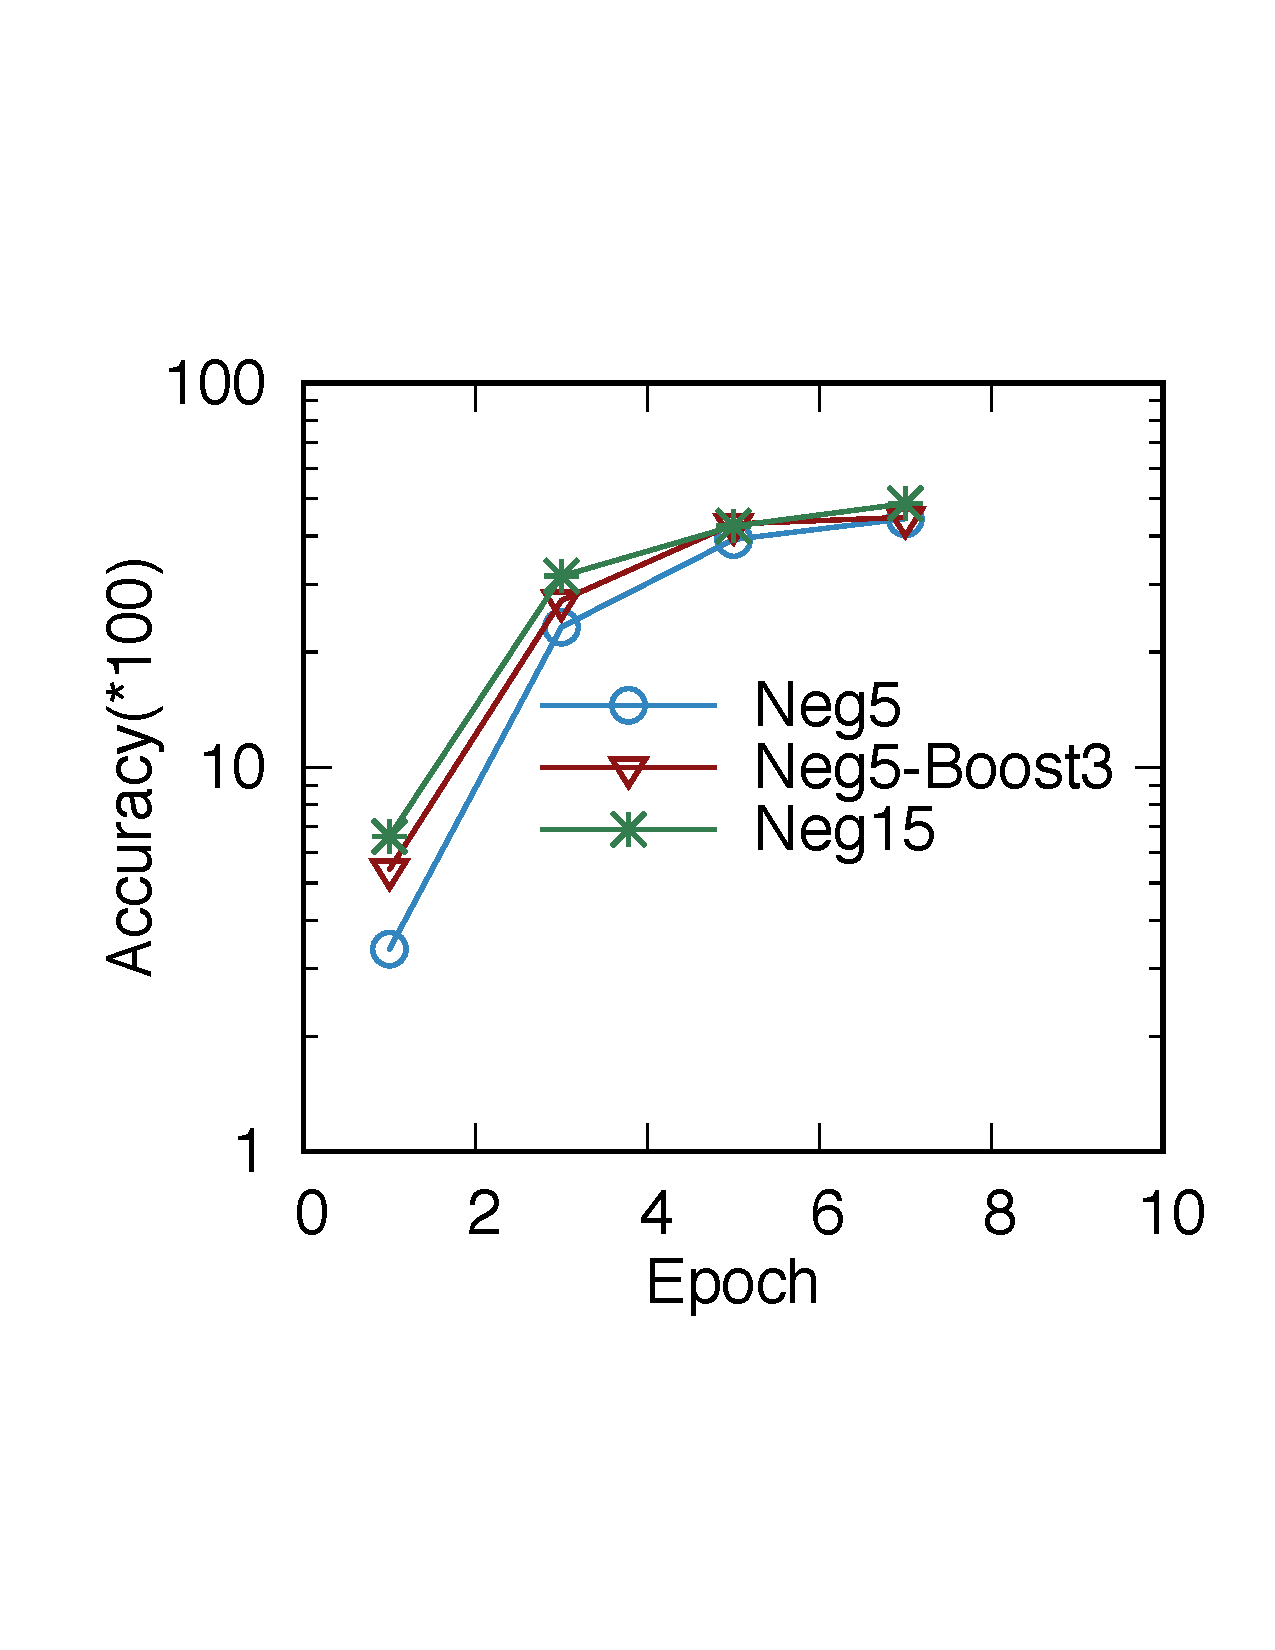
\includegraphics[width=1\linewidth]{Graph/negSamp/word2vecTask1.pdf}
% 		\vspace{-13ex}
% 		\captionof{figure}{Word analogy task: capital-common-countries.}
% 		\label{fig:wordAnaTask}
% 	\end{minipage}%
% 	\begin{minipage}{.31\textwidth}
% 		\centering
% 		\captionsetup{justification=centering,margin=0.1cm}
% 		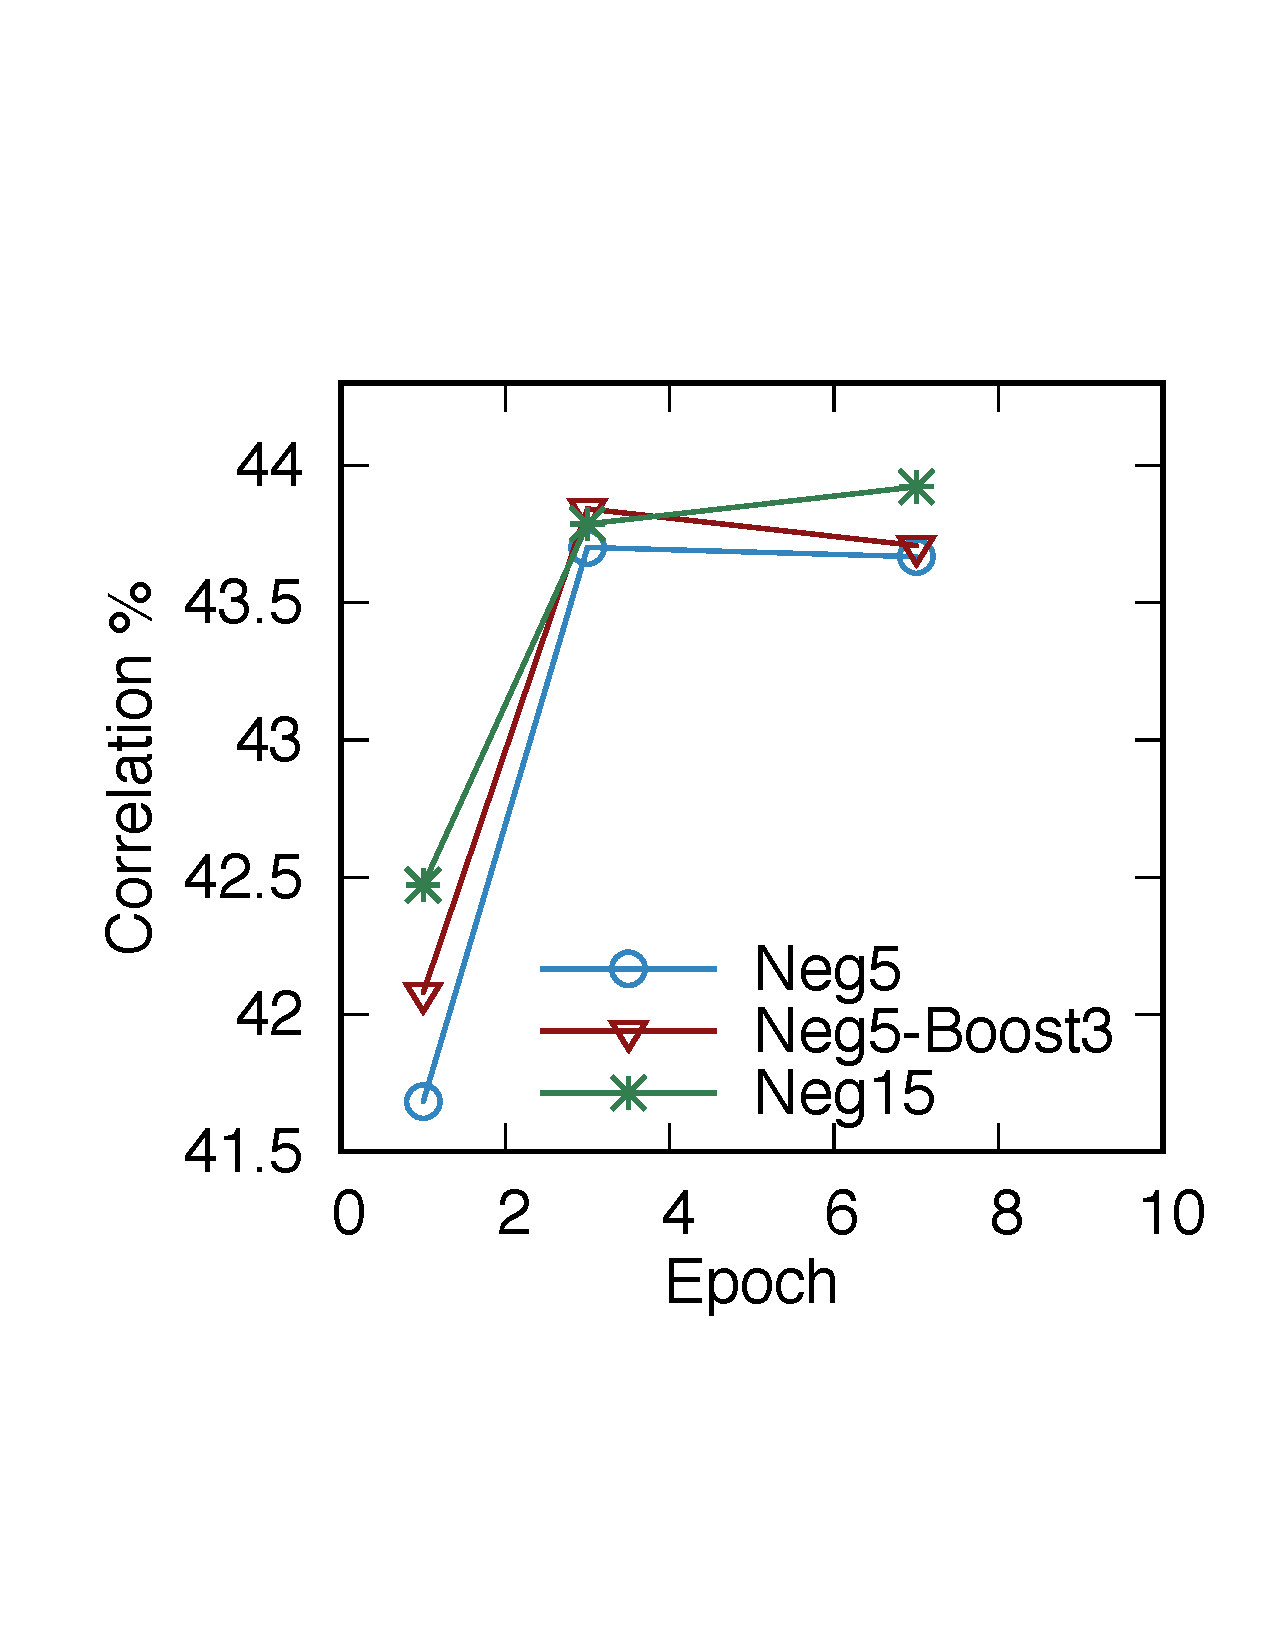
\includegraphics[width=1\linewidth]{Graph/negSamp/fasttext.pdf}
% 		\vspace{-13ex}
% 		\captionof{figure}{Fasttext: rare word's similarity.}
% 		\label{fig:fastTextSimilarWord}
% 	\end{minipage}%
% 	\begin{minipage}{.38\textwidth}
% 		\captionsetup{justification=centering,margin=0.1cm}
% 		\centering
% 		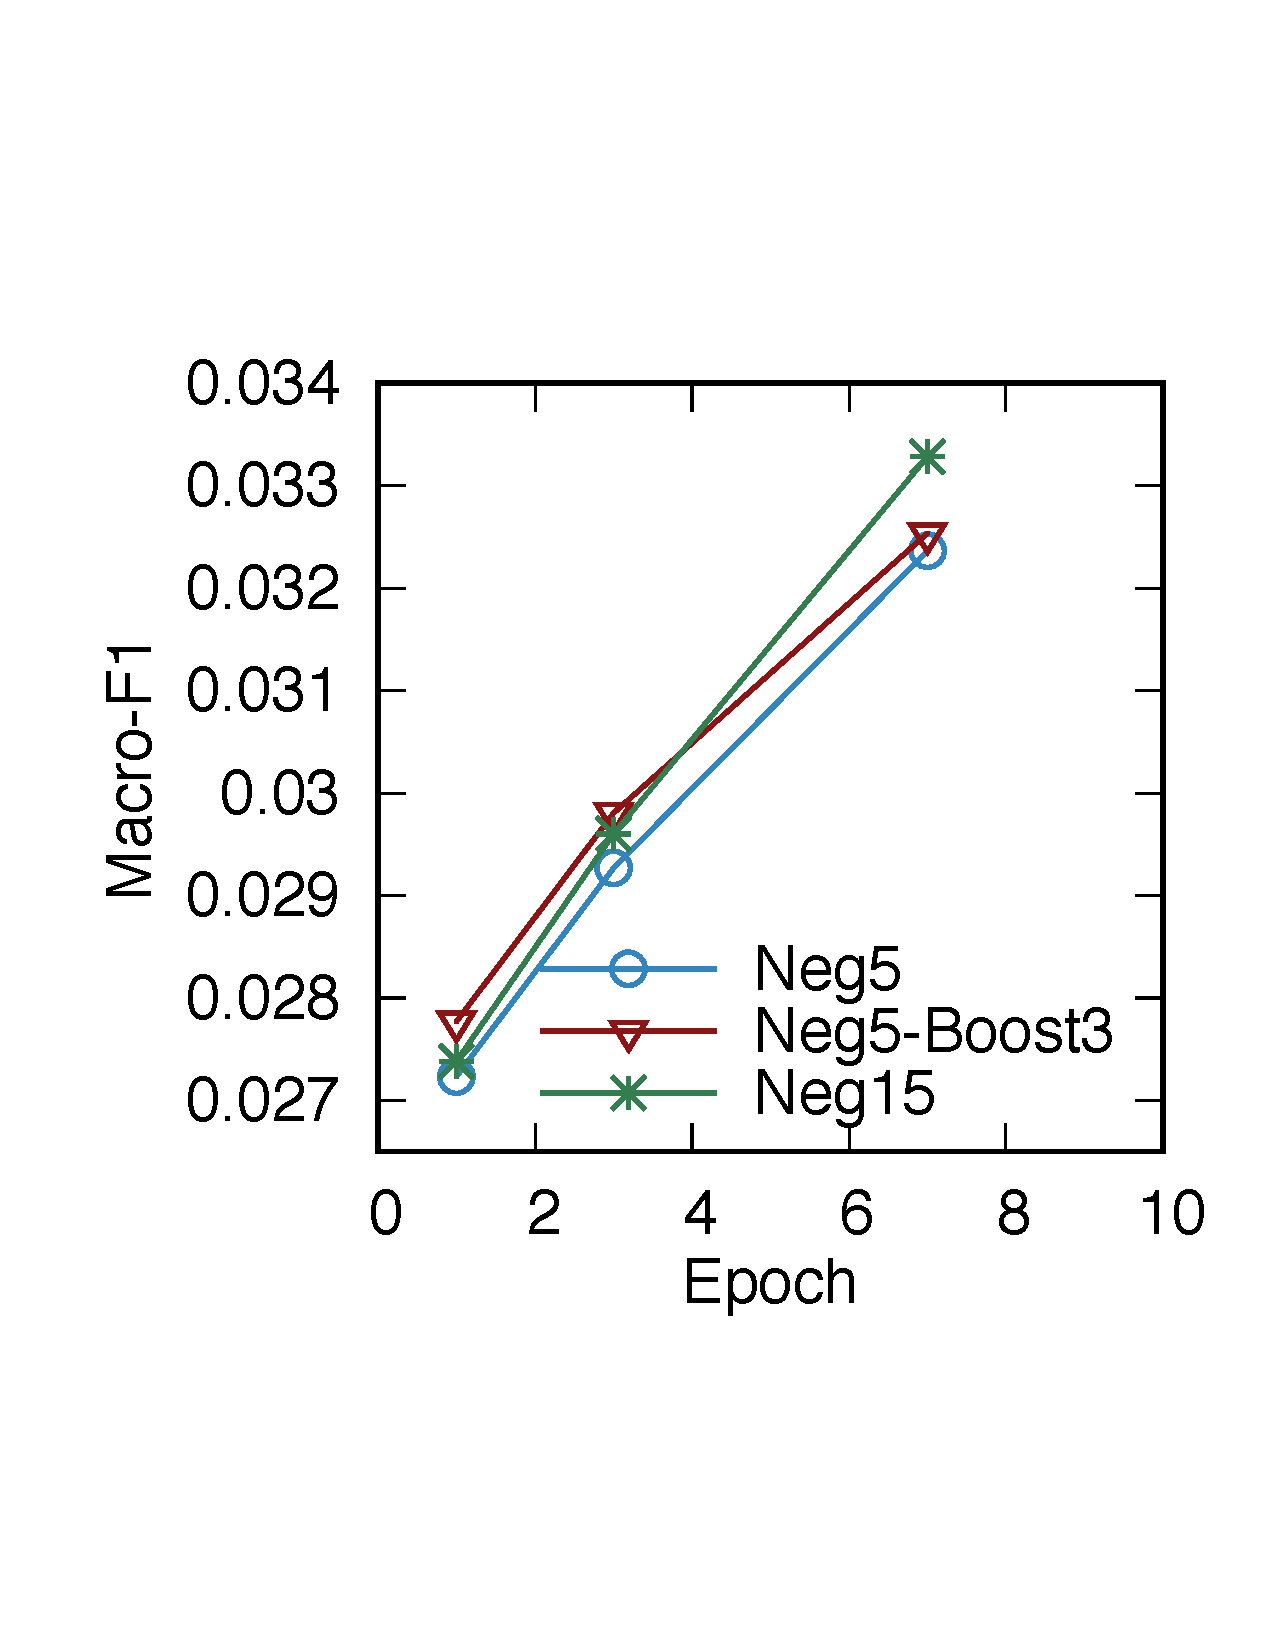
\includegraphics[width=.8\linewidth]{Graph/negSamp/node2vec.pdf}
% 		\vspace{-10ex}
% 		\captionof{figure}{Node classification.}
% 		\label{fig:nodeClassification}
% 	\end{minipage}%
% 	\vspace{-1.5em}
% \end{figure*}


% \begin{minipage}{.49\textwidth}
% %\begin{table}[h]
% \centering
%  \vspace{1.5ex}
% \captionof{table}{Word-analogy semantic-task top-1 accuracy.}
% \label{tbl:semantic}
% \scalebox{0.8}{
%  \begin{tabular}{| c |c c c|} 
%  \hline
% Task Name & Neg5 & Neg5-Amplify3 & Neg15 \\
% \hline
% capital-common-countries & 38.14 & 43.02 & \textbf{47.43}\\
% capital-world & 24.66 & 29.34 & \textbf{32.14}\\
% city-in-state & 15.17 & \textbf{17.29} & 14.93\\
% currency & 15.72 & \textbf{22.26} & 22.21\\
% family & 56.86 & 60.30 & \textbf{64.27}\\


% \hline
% \end{tabular}}
% \end{minipage}


% % \begin{minipage}{.49\textwidth}
% % %\begin{table}[h]

% % \captionof{table}{Word-analogy semantic-task top-1 accuracy.}
% % \label{tbl:semantic}
% % \scalebox{0.8}{
% %  \begin{tabular}{| c |c c c c c|} 
% %  \hline

% % Algorithm    &Task 1 & Task 2 & Task 3 & Task 4 & Task 5 \\
% % \hline
% % %  Neg5& 		37.15 &  23.21 &  14.55 &  16.42 &  52.94 \\

% % %  Neg5-Amplify3& 42.29 &  27.2 &  14.18 &  22.02 &  58.5\\

% % %  Neg15& 		47.04 &  31.47 &  16.04 &  22.15 &  65.69  \\
% %  Neg5& 		38.14 &  24.66 &  15.17 &  15.72 &  56.86 \\

% %  Neg5-Amplify3& 43.02 &  29.34 &  17.29 &  22.26 &  60.30\\

% %  Neg15& 		47.43 &  32.14 &  14.93 &  22.21 &  64.27  \\


% % \hline
% % \end{tabular}}
% % \vspace{3ex}
% % 	\end{minipage}%
% % 	\quad\quad%
% % \begin{minipage}{0.49\textwidth}
% %   \vspace{1.5ex}
% % \captionof{table}{Mapping from Task ID to task real name for word analogy semantic-task.}
% % \label{tbl:semanticName}
% % \centering
% % \scalebox{0.8}{
% % \begin{tabular}{|c | c|} 
% %  \hline

% % Task ID & Real Name   \\
% % \hline
% % 1&	capital-common-countries\\
% % 2&	capital-world\\
% % 3&	city-in-state\\
% % 4&	currency\\
% % 5&	family\\
% % % 6&	gram1-adjective-to-adverb\\
% % % 7&	gram2-opposite\\
% % % 8&	gram3-comparative\\
% % % 9&	gram4-superlative\\
% % % 10&	gram5-present-participle\\
% % % 11&	gram6-nationality-adjective\\
% % % 12&	gram7-past-tense\\
% % % 13&	gram8-plural\\
% % % 14&	gram9-plural-verbs\\

% % \hline
% % \end{tabular}}

% % \end{minipage}

% %\begin{minipage}{\textwidth}

%   \begin{minipage}{0.49\textwidth}
%   \vspace{1.5ex}
%     \captionof{table}{Training time (seconds).}
%     \label{tbl:time}
%     \centering

%         \scalebox{0.8}{
%          \begin{tabular}{|c|c c c|} 

%          \hline

%         Model & Neg5 &Neg5-Amplify3 & Neg15\\
%         \hline
%         Fasttext&736&731&1404\\
%         Word2vec&17.35&17.37&36.93\\
%         Node2vec&3.28&3.28 &4.00\\
%         \hline
%         \end{tabular}}
%     %   \captionof{table}{Training time (seconds).}
%     % \label{tbl:time}
%     \end{minipage}
% %\end{minipage}
\section{Conclustion}
In this chapter, we proposed \emph{amplified negative sampling}, a new sample-efficient method for training multi-class classifiers with a large output-class size. Our proposed method was based on our rigorous mathematical analysis. Our extensive set of experiments demonstrated that amplified negative sampling gives us the best of both worlds: It leads to the higher-accuracy model of a larger sample size without paying its high computational cost. Given its simplicity, and experimental effectiveness, we believe our proposed method will be an important extension to the widely-popular technique that results in meaningful improvements in practice.

\label{sec:NS:conclusion}

\chapter{Expressive Library for Recursive Queries: LLib and LFrame}
\label{ch:lib}


With the increasingly large volumes of data, there is an urgent need to provide expressive and efficient data analytic tools. Datalog, a declarative logical programming language, has been widely implemented  due to its superiority of concise expressing and efficient execution of recursive queries. In this chapter, we focus on extending the expressive power of the language in the data scientists' familiar ways. We propose the LLib,  Logical Libraries, to provide a wide range of Datalog algorithms on top of BigDatalog and Apache Spark.  LLib encapsulates all the complex logic of algorithms into high-level APIs to simplify the development and   provides a unified interface similar to the Spark MLlib. LLib is proposed to be  DataFrame-based so that it can flexibly collaborate with other existing Spark operations in MLlib, Spark SQL, etc.
Considering the requirements for developing novel recursive applications not contained in LLib, we also show a new LFrame-based Datalog programming interface. The LFrame is an extension to the Spark DataFrame data structure and works in the similar way. Except the normal relational operations like projection, selection, the LFrame could support  logical operations like definitions of recursive rules and base relations. To visually show the expressive power of LLib and LFrame, we utilize amounts of running examples during description. 

\section{Introduction}
In the era of big data, the demand for flexible analytics of large-scale data has driven the researchers to build various general-purpose user-friendly platforms like Apache Spark   \citep{zaharia2012resilient}, AsterixDB \citep{alsubaiee2014asterixdb}, Pig \citep{olston2008pig}, Hive \citep{thusoo2009hive}, etc.  Among these systems, Spark is getting more and more attractive due to its efficient in-memory computation and abundant APIs (i.e. Spark SQL, GraphX, MLlib and SparkR) for complex analytics  to extract the rich information encapsulated in the data.

However, for the iterative applications like identifying the transitive closures or connected components of millions of vertexes, there are no dedicated designs for optimization among recursions in Spark because each iteration is contained in an identical job.  For the more advanced recursive analytics, the programming needs deep understanding and extensive knowledge of the platform.  To solve these issues, the researchers attempt to implement the Datalog  \citep{consens1990low} systems for logical programming. 

The Datalog, a well known recursive programming language with superior expressive power, consists of a set of rules and facts. The DeALS project of UCLA \citep{yang2015parallel} implements a unified Datalog programming language and provides the parallel evaluation on multicore machines. For the distributed logical computing on clusters, the BigDatalog \citep{shkapsky2016big} system is further developed on Spark. While considering the SQL programming customs, the Recursive-aggregate-SQL (RaSQL) \citep{gu2019rasql} language is proposed as a simple extension of Spark SQL for Datalog.  


% Similarly, other systems also do not support efficient iterative computing or a unified logic-based language for concise expression. 
This torrent of Datalog platforms, however, underscores the need to provide a high-level API to simplify the development or the usage of logical programming as an important step within the data processing pipeline. In those systems, the Datalog applications run independently as one  job with input rules and datasets. It is hard for users to take the output of one Datalog program as the input for another Datalog program. Similarly, the collaboration with other Spark APIs like machine learning (MLlib), graph computation (GraphX) or the Spark SQL is inconvenient. Also, as a pre-knowledge, it is necessary for users to learn about Datalog or get used to a SQL extension (RaSQL) when they actually  want a one-line library call for a common recursive  application like transitive closure or BOM \citep{BOM} as a step of data processing. 


In this chapter, we focus on providing an ecosystem for Datalog programming on Spark, which contains LLib, wrapping normal Datalog algorithms with an easily extended interface for contributing new algorithms, and LFrame, the dataframe extension supporting the basic logical operators.  The LLib and LFrame are implemented on BigDatalog and Spark. The wide audience of Spark community should be familiar with the interface of LLib (like Spark MLlib) and LFrame (like Spark DataFrame). With LFrame and LLib, the data scientists could have access to the data manipulated in Datalog applications and easily continuously do other operations like machine learning algorithms of MLlib  within one job. This ecosystem makes it possible to ask for help from the existing Datalog algorithms by solely a one-line function calling within a processing pipeline and develop user-defined recursive application as friendly as the Pandas\citep{mckinney2010data}/Spark DataFrame. 

Our contributions can be concluded as following:
\begin{itemize}
	\item Usability. The LLib  provides functionality for a wide range of typical Datalog algorithms. It simplifies the development of end-to-end data processing pipelines with the high-level API and avoids the efforts required to learn a new language syntax.
	\item Interoperability. The LLib is the DataFrame-based API, which takes the DataFrames as the input and also generates DataFrames. This facilitate the collaborations between Datalog applications and Spark MLlib, Spark SQL or GraphX. In addition, we propose the function for the conversion between the  DataFrames and LFrames, which enhances the interoperability during data processing.
	\item Extendability and flexibility. In LLib, there is a template and some utility functions contained to help  adding extra Datalog algorithms. We also design a user-defined Datalog function for any possible Datalog applications. The LFrame data structure is associated with various general Datalog operations supporting different recursive algorithms.
\end{itemize}
The chapter is organized as follows. Section \ref{pre} reviews the basics about the Datalog language and related platforms including Apache Spark, BigDatalog and RaSQL. Section \ref{llib} describes the working paradigm of LLib,  different categories of algorithms supported by LLib, and utilizes some running examples expressing the user-defined Datalog functions and the collaborations between LLib and other Spark libraries. 
Section \ref{lframe} presents the conversion between LFrame and DataFrame, the basic unary and $N$-ary operations supported by LFrame, and some examples developed with LFrame. Section \ref{llib:conclusion} draws  conclusion and our plans for future work.


\section{Prelimiaries}


\label{pre}
\subsection{Datalog}
% base case, recursive case,
A Datalog application is comprised of a finite set of rules. Each rule $r$ is formed as H $\leftarrow l_1, l_2, ... l_n$, where H is the head of $r$, $l_{1..n}$ (the \textit{body}) are \textit{literals}   and the $\leftarrow$ means implication. The literals ($l_{1..n}$) are positive or negated atoms. One atom (H or $l_i$) can be formed as $p(t_1, .., t_k)$, where $p$ is a \textit{predicate} and $(t_1, .., t_k)$ terms can be \textit{variables}, \textit{constants} or \textit{functions}. So, the $r$ is the rule to infer H. However, if $r$ does not have the body $l_1, l_2, ... l_n$, it becomes the \textit{fact}, which corresponds to a tuple in a relation . The comma separating literals means the logical conjunction (AND). To evaluate a Datalog application, we need a \textit{query} mentioning which predicate to evaluate.

Next, we will illustrate a classic example in Datalog, single source shortest path (SSSP),  with more terms introduced. The SSSP is to calculates the length of shortest paths from one source vertex to all other vertices in a graph with weighted edges. 

\vspace{0.5em}
\qr{1} - Single source shortest path (SSSP).
\setcounter{myrow}{0}
\\
$\begin{array}{>{\quad \stepcounter   {myrow} \themyrow : \quad}lrl}

database(\{\ warc(A: integer,\  B: integer,\ Cost: integer)\ \}). \\

sp(B,\ mmin<C>) \leftarrow B=\{startvertex\},\ C=0. \\

sp(B2,\ mmin<C>)\leftarrow sp(B1, C1),\ warc(B1, B2, C2),\ C=C1+C2. \\
result(B,\ min<C>) \leftarrow sp(B, C). \\

query\ result(T, C).


\end{array}$
\vspace{0.5em}

As shown in Query 1 line 1, the input relation (\textit{base relation}) is \textsf{warc} with the schema \textsf{(A:integer, B:integer, Cost:integer)}. 
One fact of this relation can be \textsf{warc(1, 2, 5)}, which shows the  cost from    vertex 1 to 2 is 5. The \textsf{database} is a keyword specifying the base relation.
In the first rule (line~2), it initializes the shortest distance from the source vertex to itself as 0, where the ``\{startvetex\}'' can allow user to input the source vertex ID. The second rule (line~3) recursively produces all the minimum distances for all the possible paths from source node to another node. The monotonic aggregate, \textsf{mmin} is utilized, which allows the aggregation inside the recursion when set containment is satisfied. The \textsf{mmin} will get new lower value with a larger set of possible paths. And a normal aggregate \textsf{min} is finally exploited (line~4) to obtain the minimum cost path for each source vertex. The fifth line denotes the  predicate (\textit{relation}) \textsf{result(T,C)} will be evaluated and become the output of the application.

\subsection{Related Platforms: Apache Spark, BigDatalog and RaSQL}
\textbf{Apache Spark.} Apache Spark is a DISC system with various modules like Spark SQL \citep{sparksql}, Spark Streaming \citep{sparkstreaming}, MLlib \citep{meng2016mllib} and GraphX \citep{gonzalez2014graphx} to support analytics on structured data, streaming applications, machine learing algorithms and graph computation tasks respectively.  All the Spark applications are eventually represented by a series of transformations and actions on Resilient Distributed Datasets (RDDs) \citep{dean2004mapreduce}, the main abstraction provided by Spark. The operators like groupBy, filter are lazily evaluated until the output actions like count trigger evaluations on RDDs. In this way, before execution, the Spark Optimizer can design a better physical plan by avoiding some duplicate computation or pipelining operations. RDDs in Spark are actually Python or Java objects stored in memory and can be processed in parallel. The RDD is fault-tolerant due to its lineage. The lineage graph of RDDs records the transformations applied to them. When records get lost, it is easy to recover them by rerunning through the lineage graph \citep{gulzar2017automated}. The Spark has attracted wide audiences from database community due to its high usability and performance.

\textbf{BigDatalog.}
With the popularity of Spark and the benefits for recursive query evaluation and optimization brought by Datalog, the new requirements have been re-emerged to support the Datalog development on Spark. 
As far as we can find, the BigDatalog \citep{shkapsky2016big} is the first one implementing the DeALS, a Datalog platform, on Spark. It supports the execution of recursive operations on  multi-core machines and clusters. The BigDatalog also proposes some optimizations on physical planning for recursive queries to obtain the orders of magnitude speed-up. 

\textbf{RaSQL.} 
The BigDatalog enables development of Datalog on Spark, but users should get used to the Datalog syntax. With the continuing popularity of SQL, it is beneficial to design a language similar to SQL for Datalog queries. The RaSQL \citep{gu2019rasql} proposes a new language following and extending SQL standards, and utilizes some novel optimizations on fixpoint operators for the Datalog platform built on Apache Spark.  

Developing a Datalog application on BigDatalog or RaSQL  requires a query file, a structured data file, and a standard execution program, which takes the query and data files with some arguments for execution. Users are required to learn Datalog or RaSQL syntax and it is not so interoperable  between one Datalog application and another Spark MLlib, Spark SQL or Datalog application. In this chapter, we would like to  introduce the LLib and LFrame to solve those issues 
as described above.


\subsection{Spark MLlib and DataFrame}
% AFrame, DataFrame in Panda and Spark, R

The MLlib is the machine learning library of Spark. It consists of the normal classification, regression algorithms. Users can flexibly build a pipeline of a sequence of algorithms to process data with the abundant libraries in MLlib. The pipeline could span data cleaning, model initialization, training, prediction, and evaluation.  

The DataFrame is a popular facility for data scientists and has been supported by various trendy data analytics platforms and languages like Spark, Pandas~\citep{pythonDataframe}, R, etc. It is utilized as a data structure and the data stored in it is organized in rows and columns like a table in Excel. This increases the visibility of development for non-expert users. The supported operations for the DataFrame are similar to the relational algebra, but are exposed as pre-defined functions like libraries of Java, Python, etc.   

The LLib and LFrame proposed in this chapter provide a similar interface to Spark MLlib and DataFrame separately. The LLib contains the libraries for common Datalog algorithms and the LFrame is an extension to DataFrame encapsulating the normal Datalog operations like rule definition, registration of the base relations. 

\section{LLib}
\label{llib}
In this section, we discuss LLib, which works in the similar way to MLlib to develop Datalog applications. It does not require  users to be familiar with logical programming. LLib contains a wide spectrum of recursive applications including graph algorithms (Transitive Closure, i.e. \textit{TC}), temporal database queries (Interval Coalesce), financial applications (MLM),  machine learning algorithms (Logistic Regression), etc. 
The data analysts could easily take one Datalog algorithm as one step within their complex data processing process, which is more flexible than the previous distributed Datalog programming interfaces. 











\subsection{LLib Working Paradigm}
\label{sec:paradigm}
% Schema Mapping, Single DataFrame, Multiple DataFrame, Different outputs format, Arguments (Start Vetex =?)
% Wrapped DatalogSession, No need for arguments (configuration)

The LLib grants the access to the processed data to users through the Spark DataFrame, which greatly reduces the required boilerplate code and improves  the readability. In this part, we would like to firstly provide a high level picture of the difference while working on the two popular Spark-based distributed Datalog platforms (BigDatalog and RaSQL) and our LLib. 

As shown in Figure \ref{fig:comparison} (a) about the TC application, the previous Spark-based Datalog program is made up of (1) the  source data file(s), which should follow a fixed schema like  the names of fields for the corresponding application or the comma delimiter, (2) a query file following the RaSQL or BigDatalog syntax, (3) a standardized program to accept the source data file(s) and query file for recursive computation, and (4) a set of arguments to guide the program execution. This is a general-purpose design for all potential applications that can be expressed by a combination of rules running on several data files, but it causes a troublesome programming considering the following aspects.


\begin{itemize}
	\item \textit{Learning new language.} To develop with those platforms, users are required to get used to the syntax of Datalog or an extension of SQL while they actually  want to use a well-wrapped typical Datalog application as a step of their whole data processing pipeline.
	\item \textit{Data transfer.} For each application on the previous platforms, the required data need to follow a fixed schema. It costs much for the schema conversion.
	\item \textit {Isolation from other applications.} The development mode  of the original logical programming works in a way similar to a black box. Users provide data and rules to standardized program and get results. They only have access to the generated file and can hardly involve other  preprocessing or subsequent processing.  
\end{itemize}

To overcome those drawbacks, we develop the DataFrame-based LLib as shown in Figure \ref{fig:comparison} (b), which works in a similar way to Spark MLlib. Within a LLib-based application, there can be many steps made up of the permutations of regular DataFrame operations like selection or projection,  MLlib's ML algorithms or featurizations and LLib's Datalog algorithms. Later in this section, we describe the underlying architecture and working pipeline of LLib through a small running example that shows how to evaluate the transitive closure of a directed acyclic graph (DAG). 

\begin{figure}[!t]
	\centering
	\begin{subfigure}{0.7\textwidth}
		\centering
		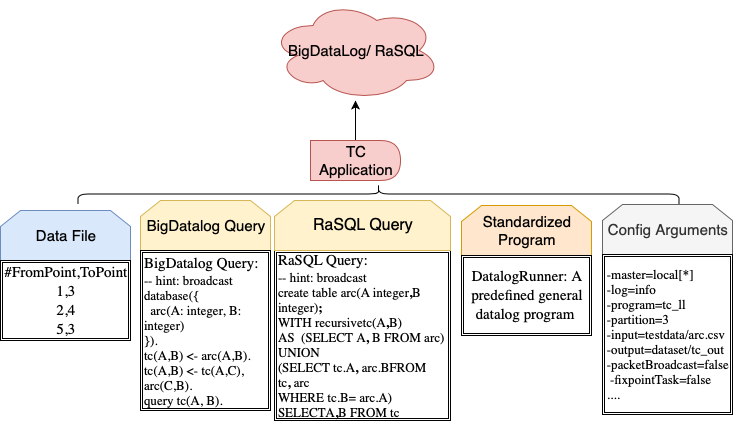
\includegraphics[width=1\linewidth]{Graph/llib/datalogPipeline.png}
		\caption{\small (a) The composition of TC application on custom Datalog platforms. } 
	\end{subfigure}%
	%   \hspace{1em}
	\vspace{\floatsep}
	
	
	\begin{subfigure}{0.6\textwidth}
		\centering
		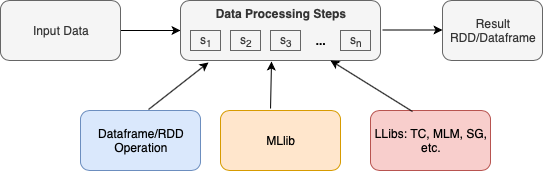
\includegraphics[width=1\linewidth]{Graph/llib/DatalogLib-4.png}
		\caption{\small(b) LLib paradigm} 
	\end{subfigure}%
	\caption{Working paradigm comparison between custom distributed Spark-Based Datalog platforms and the LLib.}\label{fig:comparison}
\end{figure}


\subsubsection{Working session and acquiring data}
\label{sec:data}
In LLib, the first step is to construct a working environment for the Datalog queries and libraries. We respect the customs of building Spark Session and exploit the similar way as following (with Transitive Closure, i.e. TC as a running example):


\vspace{0.5em}
\ex{1.1} - Transitive closure with LLIb:  Working session.
\bldl
session = LLibSession.builder(
).appName(``TC").master(``local[*]"
).getOrCreate()\\

schema = StructType(List(StructField(``Point1", IntegerType, true),\\
StructField(``Point2", IntegerType, true)))\\

df = session.read.format(``csv").option(``header",``false").schema(schema)
.load(``arc.csv")
\eldl
The \textit{LLibSession} synthesizes the  Spark environment and the special designs for logical programming. Within the same session, users are free to utilize the existing Spark libraries like MLlib  or Datalog libraries i.e. LLib. As shown in the third line, the source data can be loaded via the loading function in Spark to a DataFrame \textit{df}. 

\subsubsection{Initializing an executable object of LLib and  mapping the schema}
\textbf{Initialization: }In LLib, the pipeline of the data processing for a typical application is compressed to an object, which you can initialize and set parameters on to process  your data. In this example, we initialize a transitive closure object tc with the TC library, which is pre-defined and included in the LLib. 
Then, we can set the property by built-in functions. 

\vspace{0.5em}
\ex{1.2} - Transitive closure with LLIb:  Initializing TC.
\cldl
import\ edu.ucla.cs.wis.bigdatalog.spark.LLib.TC \\
val\ tc = new\ TC() \\

tc.setDirection(FromCol = "Node1", ToCol = "Node2")
\eldl

\textbf{Schema Mapping: }Among the built-in functions,  all the libraries are required to contain one function called setDirection for schema mapping. This is necessary because we want a more general design that can accept   DataFrame with various schemas as the input.  DataFrame may call an attribute with an arbitrary name but we need to know the corresponding relationship between its attributes and the attribute names mentioned in our library's rules. The Query 2 is a set of Datalog rules for the transitive closure. We have two attributes  From and To in the arc table in the computing logic. The two attributes can be called differently like (Node1, Node2) as shown in the df initialized in Example 1.1. The mapping between (From, To) and (Node1, Node2) can be provided by the setDirection function as shown in the third line of Example 1.2 setDirection (FromCol = "Node1", ToCol = "Node2"). If there is a long mapping list, we can easily extend the current design by  storing the mapping information within a hash table as the transferred parameter to the function.

\vspace{0.5em}
\qr{2} - Transitive closure.
\bldl
database({
	arc(From: integer, To: integer)
}).\\


tc(From,To) \leftarrow arc(From,To).\\
tc(From,To) \leftarrow tc(From,Tmp), arc(Tmp,To). \\
query\ tc(From, To).
\eldl

While processing the data with our library, we need the mapping information. But after processing, the output data's format should be consistent. There is one mechanism to rollback the schema. At the beginning of data processing, we store the schema of input data. Then, in the end, we could use the pre-stored schema to recover. 

When the amount of required attributes by the library matches the amount of columns in the input DataFrame, we could  make full use of the dataset. However, when the dataset contains more attributes than the required, it should be firstly pruned before analysis. As for the condition that the required attributes not included or the dataset contains fewer attributes than  the required, the exception will be raised.



\subsubsection{Execution and persistence}
With the executable object and imported data, the execution and persistence can be merely a one-line calling of a pre-defined function (run, genDF or genRDD) in LLib. These three functions can support the basic requirements to operate data, store the result to a variable or a file. 

\vspace{0.5em}
\ex{1.3} - Transitive closure with LLIb:  Execution and persistence.
\bldl
tc.run(df, output = "File", session) \\
val\ dfNew = tc.genDF(df, session) \\
val\ rddNew = tc.genRDD(df, session) \\

\eldl

\textbf{Execute and persist:} As shown in Example 1.3, the function $run$ is to run the logical programming and persist the result directly to the target address. In the first line, the tc operates df and store the result to File. 

\textbf{Execute and return a DataFrame/RDD:} If the user would like to keep operating the data, they would prefer to get the output data in a form of DataFrame or resilient distributed dataset (RDD) instead of persistence to files. As shown in the second and third lines of the Example 1.3, the dfNew and rddNew will be the outputs and can be further utilized for the next steps of data processing. 


These three functions are implemented for each library of LLib. They expect the input data (df) and the environment (session) as the parameters.  The session information is also needed because during execution, we want the program running within an environment with capability to support the logical 
programming. 


\subsubsection{Operate on multiple datasets}
\label{sec:multiple}
The previous showed TC example operates on only one relation, however there are many applications requiring more than one relation, which causes some changes to the  pipeline. We illustrate the Multi level Market (MLM) Bonus as a typical Datalog application \citep{mlm} acquiring more than one datasets. The application is to calculate the bonus for members of a hierarchical structural Multi Level Marketing  organization. In the organization, the new members are recruited by  and get products from the old members (sponsors). One member's bonus is based on his own sales and a ratio of the sales from the people directly or indirectly recruited by him. The scale of the ratio is a pre-defined rate. 

There are two relations in the MLM Bonus, including the \textit{sponsor} and \textit{sales}. The sponsor relation describes the recruiting relationship among the members, while the sales relation records the profits for each member. In the Datalog rules, the base case is to calculate the member's bonus by the sales table. And the recursive rule is to calculate the bonus based on the basic profits and the profits derived from the downline members.

With the help of LLib, users could implement the MLM Bonus by a pre-defined MLM class in LLib  ignoring the complex logic. The program can be as easy as the follows.

\vspace{0.5em}
\ex{2} -LLib with more than one input relation: Multi level Market Bonus.
\bldl
val\ MLM = new\ MLM() \\
MLM.setDirection(MCol = "M", ProfitCol = "P")\\
MLM.setSecDirection(MCol = "M1", M2Col = "M2") \\
MLM.run(Array(dfSales, dfSponsor), output = "resMLM", session) \\

\eldl
Suppose we already have the two relations stored in dfSales and dfSponsor. In the first line, we build an executable object of MLM. Then, we set the schema mappings for two relations in the next two lines. To operate the data and persist to resMLM file, we use the forth line calling the run function.  The run function of TC application only expects one relation as the input. While dealing with multiple relations, we aggregate the relations in an array as the input. The schema mapping is implemented by adding a new function for the second relation. However, it is possible to  maintain the schema mapping for each relation in a hash function ($h_r$) and use another hash function with the relation's name as the key and the schema mapping information (the hash function, $h_r$) as the value. 
% to store the mapping between the relation and the schema mapping hashing. 
\subsection{LLib Categories}
The supported common Datalog algorithms and utilities in LLib can be  categorized into five groups. We briefly introduce each group and the typical algorithms. 

\textbf{Graph algorithms:} The most common cases of recursive computations  belong to the graph algorithms. In LLib, the typical graph algorithms are Single Source Shortest Path (SSSP), Transitive Closure (TC), Connected Components (CC), and Count Paths (CP). The SSSP  computes the shortest paths from a specific source vertex to all other nodes in a graph with weighted edges. The length of paths are computed iteratively and there is a min aggregation to choose the shortest one. The usage of the SSSP from LLib is as follows.

\vspace{0.5em}
\ex{3} - A graph algorithm (SSSP) supported by LLIb.
\bldl
val\ SSSP = new\ SSSP() \\
SSSP.setFromVertex(vertexID = 1) \\
SSSP.setDirection(fromCol = "From", toCol = "To", costCol = "Cost") \\
SSSP.run(df, output = "resSSSP", session) \\

\eldl
The program differs from the TC example on the second line, where the source vertex is set. The remaining part of the program is identical to TC, which has been fully explained previously. 

CC is to identify the connected components of a graph by attaching and updating each node with a group ID in iterations. The group ID is set each time as the minimum node ID among the nearby nodes. The nodes in a connected component will finally share the same group ID and we just need to compute the number of distinct group IDs. In CP algorithm, we obtain the number of paths from one node to  the other nodes in a graph. The reachability  is transferred iteratively along the edges of graph. The development with CC and CP library will be similar to the TC library, where only the schema mapping is required before execution. 

\textbf{Machine learning algorithms:}
Another series of algorithms, which can be expressed by Datalog queries, are  machine learning algorithms.  Previously, the development for a simple algorithm like Linear Regression or Logistic Regression needs the intensive understanding of the Datalog. With inspirations from Spark MLlib, we provide a more declarative way to develop the machine learning algorithms (including logistic regression, linear regression, SVM, etc.)  on the Datalog platform. 
% We have shown the ML algorithms can be expressed with Datalog, but to attract a wider audience of the data science, it is important to provide a more elegant and succinct way like Spark MLlib. We provide a high-level API for the common ML algorithms including linear regression, logistic regression, etc. 
To illustrate the development with our API, we show a running example exploiting the logistic regression class.

\vspace{0.5em}
\ex{4} - Developing machine learning algorithms with LLib.
\vspace{-2em}
\bldl
//\ Import\ data. 
\\
var\ Vschema = StructType(List(StructField("Id", IntegerType, true), \\StructField(
"C", IntegerType, true),
StructField("V", DoubleType, true),\\ StructField("Y", IntegerType, true))) \\

var\ df = spark.read.format("csv").option("header", "false").schema(Vschema).load("dataV") \\
\\
//\ Training\ on\ the\ input\ relation\ df. \\
import\ edu.ucla.cs.wis.bigdatalog.spark.LLib.DL\_LogisticRegression \\
val\ lr = new\  DL\_LogisticRegression().setMaxIter(10) \\
val\ lrModel = lr.run(df, session)

\eldl
The running environment of our program is still the LLibSession. Then, we can load a pre-processed training dataset stored in a verticalized view with \textit{Vschema} (Id, F, V, T), where the Id is the identification of each training instance; the F is the feature's ID; the V is the feature's value and the T is the label. The verticalized format is beneficial for sparse training data and the transactions of Datalog rules.   After importing the required training functions for logistic regression, we could build an executable training object, \textit{lr}. The \textit{lr} wraps all the logical rules and some required relations (e.g. parameters with default value 0) of the Datalog implementation for the logistic regression training.  While initializing the lr, users can exploit the built-in functions to set the properties like the limit of  iterations, the intial value of parameters, etc. During training (\textit{run}), the session information of the Datalog environment is also required. 
% After fitting the model to \textit{df} relation, the \textit{transform} could make predictions on the testing instances with the pre-trained model \textit{lrModel}.

For comparison, we leverage the Spark MLlib for the above example. The development will become the following, which looks very similar. The differences are: 1)The  input data (\textit{dataS}) do not need verticalization and the schema is not the \textit{Vschema}; 2) An assembler is leveraged to specify the attributes belonging to the features, while in LLib, the verticalized relation is self-explanatory.; 3) The session information is not required during training, while in LLib, the session should be one input parameter for training.
Even though the differences exist, the expressing with Spark MLlib and LLib are extraordinarily similar and both user-friendly.

\vspace{0.5em}
\ex{5} - Machine learning algorithms training with Spark MLlib.
\bldl
//\ Import\ data. \\
var\ schema = StructType(List(StructField("X1", IntegerType, true), \\StructField(
"X2", IntegerType, true),
StructField("X3", DoubleType, true),\\ StructField("label", IntegerType, true))) \\

var\ df = spark.read.format("csv").option("header", "false").schema(schema).load("dataS") \\
\\
//\ Training\ on\ the\ input\ relation\ df. \\
import\ org.apache.spark.ml.Pipeline \\
import\ org.apache.spark.ml.classification.LogisticRegression \\
import\ org.apache.spark.ml.feature.VectorAssembler
\\
val\ assembler = new\ VectorAssembler()
.setInputCols(Array("X1", "X2", "X3"))\\
.setOutputCol("features") \\
val\ lr = new\  LogisticRegression().setMaxIter(10) \\
val\ pipeline = new\ Pipeline().setStages(Array(assembler, lr)) \\
val\ lrModel = pipeline.fit(df) \\
\\
% \\
% //\ Testing\  with\ pre-trained\ model. \\
%     var\ test = spark.read.format("csv").option("header", "false").schema(schema).load("test") \\
% val\ prediction = lrModel.transform(lrModel, test)

\eldl


% Before loading the data, the relation should have been stored in a verticalized view with schema (Id, C, V, Y) as introduced in Section 3.1. 

\textbf{Temporal database queries:}
LLib also supports the transactions on data related to time. For example, in the Interval Coalesce, the goal is to find the smallest set of intervals to cover the input intervals. In Datalog, users are supposed to exploit one rule to find the start points (\textit{S}) of intervals which are not inside the other intervals and another rule to recursively extend the right side of intervals, whose left side belonging to \textit{S}. However, in the LLib, the development will be as simple as follows with \textit{df} (S and E column represents the start point and end point) as the input intervals and the \textit{session} built by LLibSession.


\vspace{0.5em}
\ex{6} - Temporal database query with LLib.
\bldl
val\ Coalesce = new\ Coalesce() \\
Coalesce.setDirection(startCol = "S", endCol = "E") \\
Coalesce.run(df, output = "res", session)
\eldl

\textbf{Financial   applications:}
Except the MLM Bonus mentioned in Section \ref{sec:multiple}, we also support the other financial applications like Bill of Matreials (BOM) \citep{BOM} and  Management. In BOM, one input relation is \textit{assembling} table recording the assembling relation between one item $i$ (or a part of $i$) and its immediate subparts. Another input is \textit{basic} table recording the time cost to deliver the basic parts. The task can be calculating the days required to get  the $i$ ready. We can obtain the required time for each subpart of $i$ and use the maximum time as the result. The calculating of time for each subpart of $i$ should be  execute recursively. In Management, the input table stores the manager and the employees managed by them, and the task is to calculate the total account of employees directly or indirectly managed by one manager. This also requires recursive execution. In LLib, we provide a class wrapping the execution of the BOM or Management and the usage will be similar to the example introduced in Section \ref{sec:paradigm}.

\textbf{Other applications:}
Some other important and classical recursive query applications are also contained in LLib, like same-generation (SG), which identifies pairs of humans with the same hop distance to a common ancestor.  The working paradigm with them will be similar to the Spark MLlib and same as the examples in Section \ref{sec:paradigm}. Here, we will not make repetitive illustrations.

\subsection{Extension of LLib}
LLib also provides a unified template, \textit{TempLib}, to follow when contributing a new algorithm to the LLib. All existing algorithms are developed based on the TempLib. In the TempLib, the provided non-abstract utility functions (like arguments parsing function) can be easily exploited while developing a new algorithm. The template as well contains some requirements needed to be followed. The implementation should at least include three functions (run, genDF and genRDD) for execution and persistence. With the template, the implementation becomes quite uncomplicated. As long as users have the Datalog rules for the algorithm, they can add their own algorithm by doing some minor changes to the existing codes for algorithms like TC. The changes may include a different schema mapping function, or a new function to set an input parameter for your application like the function to set the starting point in the SSSP. 

\subsection{Collaboration with other applications}
The input and output relations in LLib can be both DataFrames, which makes it possible to add a preprocessing  providing the input DataFrames  or  a subsequent processing which takes the DataFrame generated from LLib. The LLib allows users to exploit the Datalog application as a simple step at any place of their  processing pipelines. In this section, we illustrate a concrete example showing the collaborations between LLib and other applications like Spark MLlib or Spark DataFrame Operations. The showed LLib application is the BOM application mentioned previously, and we want to use the linear regression library from MLlib to get the relation between the assembling days and the price of one part. To save the space, we do not show the process to build the session (LLibSession), and load three input relations (dfAssbl, dfBasic, partPrice).  The dfAssbl and dfBasic are two relations in the BOM application storing the assembling relations among parts and the delivery time for basic parts. The partPrice stores the price for each part. With Delivery class from LLib, we could get the \textit{dfRes} storing the cost time for each part. Joining the result relation with the partPrice on the part column will generate a new relation with columns of the day and price. The Linear Regression function from MLlib could train on the result DataFrame. In this example, we can find the  LLib is able to collaborate fluently with other operations in Spark like MLlib (LinearRegression), DataFrame Operations (join).

\vspace{0.5em}
\ex{7} - Collaboration between LLib with other Spark libraries.
\bldl
dfAssbl = dfAssbl.where("Sub < 7")\\
val\ Delivery = new\ Delivery()\\
Delivery.setDirection(PartCol = "Part", SubCol = "Sub")\\
Delivery.setSecDirection(PartCol = "Part", DaysCol = "Days")\\
val\ dfRes = Delivery.genDF(Array(dfAssbl, dfBasic), session)\\
val\ dfRes = dfRes.join(pricePart)\\ 
val\ parsedData = dfRes.rdd.map(row=>\\ LabeledPoint(
row.getAs[Int]("Days"),
Vectors.dense((row.getAs[Int]("Price")))
))\\
val\ numIterations = 10 \\
val\ stepSize = 0.00000001 \\

val\ model = LinearRegressionWithSGD.train(
parsedData,
numIterations,
stepSize)\\

model.save(session.sparkContext, "scalaLinearRegressionWithSGDModel")\\


\eldl



\subsection{Multiple Datalog applications}
A Datalog application can not only work with other Spark libraries but also work with other Datalog applications. The working paradigms of multiple Datalog applications can be in sequential or orthogonal ordering. When they work in sequence, one Datalog application will take another one's result dataset as the input. If they work in an orthogonal ordering, one application's input will be irrelevant with the data processed in other Datalog applications. Both the working paradigms can work with the LLib library, as the library operate on the DataFrame and it is simple to transfer data among applications. This cannot be achieved with the previous Datalog platforms, for they take each Datlog application as a single job to execute, which can hardly collaborate. 

\subsection{User Defined Datalog Function}
Although we have provided all the common Datalog functions in our mind, users may also want to define their own function so that they can use it for futural development. To serve the user-defined datalog function (UDDF), we provide two general classes SingleTableUDDF and MultipleTablesUDDF, which wrap the necessary components to execute the Datalog queries and persist the results to files or a new DataFrame.  The SingleTable is exploited when the UDDF has one input relation while the MultipleTables is exploited when the UUDF has more than one input relations. While utilizing the two classes to specify new Datalog applications, the only required information include Datalog rules and the schema of the basic table (or input table).  

We will show the UDDF with a running example as follows. In the Example 8, we suppose user want to define their SG and Delivery application.   Suppose the \textit{df} stores the  parent-children relations among people. The \textit{dfAssbl}, \textit{dfBasic} stores the assembling relation among parts and the cost days to deliver the basic parts.  The session is a LLibSession. The process to create the df, dfAssbl, dfBasic and session is omitted. For the UDDF of SG, we build an executable object by the SinlgeTableUDDF class and specify the input relation's schema by registerDatalogTable function. The rules are  provided afterwards, which contain the input relation. During execution, the input table (df) and the  query to trigger the  table persistence should be provided. Similarly, for the Delivery, expecting dfAssbl and dfBasic as the input datasets, users are required to build an executable object and register two relations separated by the comma signal. The exeuction can be trigger once the rules and final query are provided. The two executable object (UDDFSG, UDDFDelivery)  are reusable for the future development. If necessary,  users can  build as many UDDFs as they want in a single program.


\vspace{0.5em}
\ex{8} - User-defined Datalog functions.
\bldl
//\ Datalog\ application\ with\ one\ table. \\
val\ UDDFSG = new\ SingleTableUDDF() \\
UDDFSG.registerDatalogTable("rel(Parent: integer, Child: integer)") \\
UDDFSG.rule("sg(X,Y) \leftarrow rel(Parent,X), rel(Parent,Y), X ~= Y. sg(X,Y) \leftarrow rel(A,X),\\ sg(A,B), rel(B,Y).") \\
UDDFSG.run(sourceDataFrame = df, output = "UDDFSG", session, query = "sg(X, Y).") \\
\\

//\ Datalog\ application\ with\ multiple\ tables. \\
val\ UDDFDelivery = new\ MultipleTablesUDDF() \\
UDDFDelivery.registerDatalogTables("  assbl(Part: integer, Sub: integer),\\ basic(Part: integer, Days: integer)")\\
UDDFDelivery.rule("actualdays(Part, mmax<Days>) \leftarrow basic(Part, Days).\\ actualdays(Part, mmax<Days>) \leftarrow assbl(Part, Sub), actualdays(Sub, Days).")\\
UDDFDelivery.run( Array(dfAssbl, dfBasic), output = "UDDFDelivery", session,  \\query = "actualdays(P, D).")




\eldl



\section{LFrame}
\label{lframe}
DataFrame, a widely used data structure, is always supported in different data analytic facilities like Spark SQL, R, Python, but not in Datalog platforms. In this section, we provide a data structure LFrame, wrapping both the Datalog transactions and the common DataFrame transactions. The rest is organized as follows: Section \ref{sec:utility} describes how to convert a normal DataFrame variable to the LFrame variable. Section  \ref{sec:unary} discusses unary operations that operate on one LFrame, while the Section \ref{sec:nary} discusses the N-ary operations using with more than one  LFrame. In each of the Section \ref{sec:unary} and Section  \ref{sec:nary}, we describe one concrete example to illustrate the development with LFrame.

% In Section \ref{sec:expLFrame}, we describe two concrete examples to illustrate the development with LFrame.


\subsection{Conversion from DataFrame to LFrame}
\label{sec:utility}
% Single Frame, Different Frames
To build an LFrame variable, we show the process by the following example.
The entry point of the application using LFrame is the LLibSession, same as the one in LLib, which makes it possible to use both LLib and LFrame within one execution environment. 
The session can  load the data to a DataFrame variable df, but the df cannot execute any logical transaction. To construct an LFrame variable with the  df, a built-in function wrapperDF in LLibSession can be utilized with the session and df as the inputs. 
The session is transferred to provide the Datalog running environment and the df is to supply the dataset with schema.  
The constructed LFrame variable, lframe, could support various Datalog operations like specifying the rules, input tables, persisting the result to a file, etc. These operations are categorised to unary operations and $N$-ary operations and introduced later.

\vspace{0.5em}
\ex{9.1} - Development with LFrame:  Conversion from DataFrame to LFrame.
\bldl
val\ session = LLibSession.builder().appName("LFrame").master("local[*]").getOrCreate() \\
var\ schema = StructType(List(StructField("Parent", IntegerType, true),\\ \ StructField("Child", IntegerType, true)))\\
var\ df = session.read.format("csv").option("header", "false").schema(schema).load("sg")\\
var\ lframe = LLibSession.wrapperDF(df, session)
\eldl

\subsection{LFrame: Unary Operation}
\label{sec:unary}
The unary operation only involves one LFrame object each time. With the lframe in Sec. \ref{sec:utility}, we implement the SG application as following to show the typical provided unary operations. 


\vspace{0.5em}
\ex{9.2} - Development with LFrame:  Unary operations with SG application.
\setcounter{myrow}{0}
\\

$\begin{array}{>{\stepcounter   {myrow} \themyrow : \quad}lrl}
//\ Datalog\ operations\ for \ SG\ application. \\
lframe = lframe.registerCurLFrame("lframe1(Parent: integer, Chile: integer)")\\
lframe = lframe.rules("sg(X,Y) \leftarrow lframe1(Parent,X), lframe1(Parent,Y), X ~= Y")\\
lframe = lframe.rules("sg(X,Y) \leftarrow rel(A,X), sg(A,B), rel(B,Y)")\\
lframe = lframe.rules("sg(X,Y) \leftarrow sg(X,Y)")\\
lframe = lframe.delRule(3)\\
lframe = lframe.query("sg(X,Y)")\\
\\
//\ Execution\ and\ persistence. \\
lframe.run(output = "SG")\\
val\ dfRes = lframe.genDF()\\
val\ rddRes = lframe.genRDD()
\\ \\
//\ Normal\ DataFrame\ operations. \\
lframe.nonRecursive().where("X < 10").select("X").collect().foreach(println) \\
\end{array}$
\\

There are six categories of unary operations included in the above example. 
\begin{itemize}
	\item \textbf{Registering one LFrame as a base relation.} In the line 2, the registerCurLFrame is to register the lframe as a base relation so that the Datalog rules can utilize it as a given dataset. While registering, users are free to rename the dataset's columns and the LFrame will map the columns according to the order of appearance. 
	\item \textbf{Appending rules.} The main body (line~3 to~5) of a Datalog program is a finite set of rules. To state the rules, the function called "rules" can be exploited. Whenever the function is utilized,  a new rule will be appended to the existing rule sets owned by the lframe.
	\item \textbf{Removing rules.} If one rule is wrongly appended, it can be removed by the delRule (line 6) function using its index. The provided index variable can be also an array, which removes more than one rule.
	\item \textbf{Specifying output relation.} To evaluate the application, the query function (line 7)  assists to point out the output relation, which is the sg relation in the SG application. The generated result LFrame will store the output dataset in the schema specified in query, (X, Y).  
	\item \textbf{Execution and persistence.} In DataFrame, the evaluations are lazy. Similarly, the LFrame's evaluation is lazy until the run action is triggered.  As shown in the second part of the code (line~9 to~12), the run function will store the result relation to a file and if a user want to restore the result to a DataFrame or RDD, the genDF or genRDD function can be considered. 
	\item \textbf{Non-recursive transactions.} The design of LFrame is to wrap both the Datalog transactions and the normal DataFrame transactions. When a normal DataFrame transaction is required, like the line 15 shows, the nonRecusive function will convert the execution to the normal DataFrame execution and accept all the DataFrame operators afterwards. 
\end{itemize}
Compare the LFrame with DataFrame, we can find they work in  analogous ways  but LFrame can support more operations. A more compact way to express the transactions from line 2 to 7 is to list them back to the lframe one by one like the line 15. 
\subsection{LFrame: N-ary Operation}
\label{sec:nary}
In the previous SG example, only one relation is contained in the Datalog application, while in this section, we illustrate the transaction (registerMoreDFs)  embroiling more relations like the join operator of the relational database or DataFrame. We adopt the Delivery Datalog application as a running example, for it contains both the assembly and the basic relations. The assembly relation stores assembling relation among parts and the delivery days of basic parts are stored in the basic relation. The expected output should be the  time spent for each part.

\vspace{0.5em}
\ex{9.3} - Development with LFrame:  $N$-ary operations with Delivery application.
\setcounter{myrow}{0}
\\

$\begin{array}{>{\stepcounter   {myrow} \themyrow : \quad}lrl}
var\ schemaAssbl = StructType(List(StructField("Part", IntegerType, true),\\ \quad StructField("Sub", IntegerType, true)))\\
var\ dfAssbl = session.read.format("csv").option("header", "false").\\ \quad schema(schemaAssbl).load("assbl")\\
var\ schemaBasic = StructType(List(StructField("Part", IntegerType, true),\\ \quad StructField("Days", IntegerType, true)))\\
var\ dfBasic = session.read.format("csv").\\ \quad option("header", "false").schema(schemaBasic).load("basic.csv")\\
\\
//\ Datalog\ operations\ for \ Delivery\ application. \\
var\ lfAssembly = DatalogLibSession.wrapperDF(dfAssbl, session) \\
lfAssembly = lfAssembly.registerCurDF("assbl(Part: integer, Sub: integer)")\\
lfAssembly = lfAssembly.\textbf{registerMoreDFs}(otherDF = Array(dfBasic), \\ \quad registers = Array("basic(Part: integer, Days: integer)"))  \\
lfAssembly = lfAssembly.rules("actualdays(Part, mmax<Days>) \\ \quad \leftarrow basic(Part, Days)") \\
lfAssembly = lfAssembly.rules("actualdays(Part, mmax<Days>) \\ \quad \leftarrow assbl(Part, Sub), actualdays(Sub, Days)")\\
lfAssembly = lfAssembly.query("actualdays(P, D)")\\
lfAssembly.run(output = "Delivery_1")\\


\end{array}$
\\

In the example, we do not show the process of establishing the execution environment (session) to save space. We firstly load two relations to DataFrame objects dfAssbl and dfBasic (line~1 to~8). Then, the dfAssbl is converted to an LFrame variable with Datalog functions encapsulated. To exploit the relation as the base relation, the registerCurDF function is exploited in line 12. 

The above mentioned steps solely rely on one relation, however, the basic relation is required in the Delivery application. To involve more datasets, the registerMoreDFs function (line~13) need to be utilized. The input parameters include an array of DataFrames to be registered and another array of schemas exploited to register them. The two arrays are ordered and have one-to-one correspondence. Thereupon, the rules can take these DataFrames as the base relations to use. To construct the rule sets, the rules function is adopted multiple times. Eventually, the output relation specified by query function will be stored to the address contained in the run function (line~19 to~20). 

% Binary: 2
% Ternary: 3


% Single Frame, Different Frames


\section{Conclusion}
\label{llib:conclusion}

In this chapter, we have shown the LLib encapsulating typical Datalog algorithms, which follows the data scientists' customs  and requires less logical programming expertise.  For the possible  extensions of LLib, we provide not only a unified template for normalizing the contribution, but also some utilities to simplify the extending process.  With some running examples, we  demonstrate the benefit of designing the LLib as the DataFrame-based API is that the Datalog algorithm can  become a single step within the data processing pipelines collaborating with other Spark operations. For the audience who has more logical programming experience and would like to design their own applications, we also provide an LFrame API containing both logical and DataFrame-based operations. A simple conversion approach between the DataFrame and LFrame is also given for a simplified developing. Moving forward, we have  plenty of new algorithms and logical oeprations to add for the LLib and LFrame separately. We plan to make the LLib and LFrame more general for different languages like Python, R. We also  would like to implement the two interfaces on other distributed platforms or crossing various platforms in a way like a polystore system \citep{duggan2015bigdawg}



\chapter{Conclusion}
\label{ch:con}

In this dissertation, we have presented models to extract information with involvement of unused data for the optimal downstream task performance. We also discussed the approaches to improve the efficiency of  developing analytics algorithms with complex recursions and training large-class classifiers for the big data. In this section, we will wrap up the dissertation and suggest some avenues for future research.
%training deep neural networks efficiently for large-class classifier 

In Chapter \ref{ch:dip}, we discussed the way to include the IP address sequences in the internet embedding by deep learning, which we found could tackle the issue of missing information for locating unknown IP addresses and provide sufficient coverage of  protected networks in denial-of-service attacks. We discovered the hidden structural information encoded in a node's IPv4 address. To extract the encoded information, we designed a deep learning based framework, DIP, which is a ten-layer neural network and a variant of RNN. During the training of DIP, we jointly utilized the IP address, hop count and routing information and used the distance estimation as the objective. With experiments on  test data, we found the learned embedding vectors  could preserve the real-world clustering of the associated nodes and predict distance between them accurately. Moreover, for unknown hosts, DIP could accurately impute hop count distance to them merely by their IP addresses and routable prefixes. These findings inspired us to apply DIP on hop count filtering based spoofing detection, a classical framework in network security. We reviewed the previous design of spoofing detection with the explicitly computed IP maps, the collection of  immutable structural network properties  among IPs like hop counts.  Since DIP could learn the embedding of internet and predict the structural properties of arbitrary IPs, the DIP-based detection mechanism could save the time of measuring the structural properties to build up  IP maps and increase the coverage of protected hosts. 

In Chapter \ref{ch:nbest}, we discussed the way to include the 2$^{nd}$-$n^{th}$ best hypotheses generated by ASR module in SLU pipeline, which we found  could improve the SLU system robustness to ASR errors. In a conventional SLU system, the ASR module transcribes the input speech to sentences (hypotheses)  and the hypothesis with highest confidence score will be transferred to natural language understanding module. We argued that solely relying on the best hypothesis could be erroneous, which could be revealed from  the spoken recognition quality distribution. We reviewed the existing approaches to utilize $n$ hypotheses, among which  the reranking model is the most popular one. With motivating examples, we demonstrated the condition that reranking model cannot figure out. To tackle the issue, we tried integrating the hypothesized texts and embedding vectors in numerous models. Among the developed models, the PoolingAvg, which concatenated the embedding vectors and used a average pooling layer to generate a unified vector, outperformed all the others.  The PoolingAvg achieved significant classification accuracy improvement for downstream tasks including domain classification and intent classification. We also observed that with more hypotheses combined, the performance could be further improved. 

In Chapter \ref{ch:nec}, we addressed the expensive computational cost to train a large-class classifier for a big data set. When a classifier is modeled as a neural network, it is always represented by a softmax layer. The softmax layer training is the main reason for the high cost due to its intractable normalization constant. We gave a thorough overview of  the  negative sampling, hierarchical softmax, adaptive softmax to approximate the softmax.  We proposed the amplified negative sampling by introducing the amplifing factor to the known negative sampling. With experiments on real-world datasets and tasks, we showed the efficiency of the amplified negative sampling on both the sampling cost savings and performance  boosting. 

In Chapter \ref{ch:lib}, we demonstrated an expressive interface for succinct development of complex analytics with recursions.  We introduced the superiority of Datalog systems on expressing recursive queries and overviewed the latest Datalog systems, including BigDatalog, RaSQL. Although much effort has been taken to optimize the scalable logical operations  within distributed Datalog environment and to  design a better interface to extend the expressive power, there is still space to improve the usability considering  "normal" data analysts. We provide the cross-language libraries, i.e. LLib and LFrame. The LLib, similar to Spark MLlib,  encapsulates common Datalog applications for an end-to-end development. The LFrame, an extension to Spark DataFrame, supported both relational and logical operations. With running examples, we showed the interface helped data scientists  efficiently develop succinct recursive analyzing algorithms with a familiar environment.


All together, we are really excited about all the progress made in the big data analytics systems and algorithms  and glad to be able to contribute to this. We do think there is still a long way to go and would like to point out the avenues for future research in our mind.

\textbf{More available but unused information.}  In the dissertation, we introduce the unrecognized information in conventional algorithms of two domains, however we believe this is common in other domains. Here, we would like to keep sharing our other observations of  the two domains  and hope these could encourage more upcoming research works in those areas or more. 
 
As for the SLU, the first type of information can be helpful is the acoustic-model information like confidence score, which is ignored in our current hypotheses integration models but shown to be informative in other speech applications \citep{kumar2014normalization, fiscus1997post}. The recognized hypotheses from ASR module are associated with confidence scores, which tell the quality of each hypothesis. The confidence scores exist in different  layers, for example, the  confidence score of $i^{th}$ best hypothesis or the  confidence score of the $j^{th}$ word in the $i^{th}$ best hypothesis. The PoolingAvg approach treats each hypothesis equally although the quality of the hypotheses actually varies. We thus need to consider a new design to hierarchically involve the multi-layer acoustic-model information for a more efficient integration. The second direction is to use deep learning framework on word lattice \citep{liu2014efficient} or confusion network \citep{hakkani2006beyond, tur2002improving}. The hypotheses are derived from the word lattice or confusion network, so they may contain more information like times.  

As for the internet embedding, since we have proposed the DIP and the neural network can be easily extended for other data sources, we could use the other latency measurements \citep{vivaldi} more than hop counts by simply changing the cost function of the DIP.  In addition, the AS membership information could provide a coarse indication of locality of IPs \citep{barford-infocom}. We could adapt the AS membership as another estimating error within the internet embedding algorithm.

\textbf{Multi-task learning.}  Besides involving the extra information, there is also opportunity to consider more relevant tasks by multi-task learning (MTL),  which generalizes the learned model and broadcasts the knowledge among multiple fields. MTL \citep{zhang2017survey,liu2019multi,caruana1997multitask} is a widely used machine learning paradigm for training multiple related tasks in the same time. The superiority of MTL is to avoid  overfitting and transfer knowledge. This could inspire us to add more tasks for the model training. For example, in  SLU,  we can consider a new task to reconstruct the ground-truth transcription using the hypotheses.  The common tasks for hypothesis embedding model are natural language understanding tasks (domain or intent classification or slot filling), while the transcription reconstruction can help recover the error contained in hypotheses for a better understanding.

\textbf{Multi-platform data analytics.}  Our LLib and LFrame could support data scientists' familiar development with multiple programming languages, while another need to support multi-platform programs keeps increasing. For example, while detecting abnormal exchanges of stock market with real-time platforms such as Spark Streaming \citep{zaharia2013discretized}, users may be interested in retrieving historical stock data stored in a NoSQL databases like MongoDB \citep{chodorow2013mongodb}. To support the cross-storage-system queries, the ploystore \citep{duggan2015bigdawg} architecture was proposed. Following this trend, for more succinct recursive query analysis, we could try to build a Datalog-based polystore system, which should be extensible to various platforms like Spark, MongoDB, etc.

I hope this dissertation could inspire the research in deep learning and scalable  data analytics. Furthermore, I hope the embedding approaches, training algorithms and libraries constructed could contribute to both academic and industrial applications. 




\phantomsection
\addcontentsline{toc}{chapter}{Bibliograpy}

\bibliographystyle{apa}
\bibliography{thesis}    % bibliography references

\end{document}

